\documentclass{MSthesis} 
% subclass of the document class report.
\pgfplotsset{compat=1.16}

%\def\checkmark{\tikz\fill[scale=0.4](0,.35) -- (.25,0) -- (1,.7) -- (.25,.15) -- cycle;} 
\def\scalecheck{\resizebox{\widthof{\checkmark}*\ratio{\widthof{x}}{\widthof{\normalsize x}}}{!}{\checkmark}}
%that's defined it - now for a test

\begin{document}

% Formatting titles and spaces 

% Originally its
% Chapter 1:
% Name of chapter one
\titleformat{\chapter}[hang] 
{\normalfont\huge\bfseries}{\thechapter}{1em}{}  

% left margin, vertical space,  space to section, 
\titlespacing*{\chapter}{0cm}{0cm}{0cm}
\titlespacing*{\section}{0cm}{0cm}{0cm}
\titlespacing*{\subsection}{0cm}{0cm}{0cm}
\titlespacing*{\subsubsection}{0cm}{0cm}{0cm}
%%%%%%%%%%%%%%%%%%%%%%%%%%%%%%%%%%%%%%%%%%%%%%%%

% USING THE TWOSIDED OPTION left = inner , and right = outer
\myfrontpage
\mycopyright
%\newpage\null\thispagestyle{empty}\newpage

% Abstract should have first page nr,
\pagenumbering{roman}
%\chapter*{Abstract}
\addcontentsline{toc}{chapter}{Abstract}
Ikke skriv masteroppgaven som om LSTM kommer til å funke. Skriv generelt at i denne oppgaven skal vi test to metoder. Hugo. 
Skriv også om alle valg som er tatt i hensyn til når du lager datasettet. Dette er viktigere enn sykt mye teoridel. 


\subsection*{Introduce topic and why its important}
Over the last decades researchers have been working on determining the climate sensitivity. The fifth assessment report result in a range of 1.5K to 4.7K. Here 4.7K allows for a doubling of the $CO_2$ emissions compared to 1.5K. Most of this uncertainty is attributed to how clouds are resolved in climate models. (Her har jeg vell sagt motsatt ting.) We known clouds are important in today's climate. They reflect 50\% of the solar radiation back into space. %Trap less heat because of global warming. 

\subsection*{Introduce a challenge or unresolved issue that you will try and solve.} 
Large uncertainties associated with the effect of clouds in future climates. Its unclear to which level of sophistication these sub-grid scale parametrizations need to be in order model their effect on climate.

\subsection*{What have you done to try and solving this.}
In order to investigate the data driven learning potensial for parameterisation of clouds, a new dataset (European Cloud Cover) was compiled. Methods like traditional statistical models and ConvLSTM was used to relate simple meterorological surface variables to cloud cover. The sophistication of a parameterisation is never know a-priori.

\subsection*{Main result - Include the numerical result of your best model.}

\subsection*{The implications in the context of 1+2.}
\cleardoublepage
\chapter*{Acknowledgement}
\addcontentsline{toc}{chapter}{Acknowledgement}
This thesis is a joint work between \acrfull{uio}, \acrfull{simulamet} and \acrfull{oslomet}. First and foremost I would like to thank my supervisors Hugo L. Hammer (\acrshort{oslomet}), Trude Storelvmo (\acrshort{uio}) and Michael Riegler (\acrshort{simulamet}) for giving so much freedom to make my own choices regarding the data.

Thanks to Hugo and Michael for suggesting this interesting topic of \textit{Applying artificial intelligence to perform climate predictions}, and to Trude for joining us, allowing me to shift the focus toward applications to cloudphysics.

I would also like to thank Raymond Wiker, Jonah Shaw and Ina Storteig for their support and comments. Your contribution have been valuable for my work.

A big thanks goes to my fellow master students, friends and family. Your support have been great.
 
I would also like to thank the scientist at EUMETSAT. 
Their expertise have been invaluable when generating the data set. 
The IT-support on the GEO-department your technical support regarding storage space and other stuff related to this. 

Finally, the constant encouragement of my sister, Sara, is sincerely appreciated.
%A big thanks goes to my sister Sara for her unconditional support and for occasionally keeping me company as MetOs. Its much appreciated. 
%Thanks to Michael Schulz and Jan Griesfeller for giving me access to Modis6.1 Terra data, prepossessing the data. 
%Kind and patient supervisors for listening to \textit{all my great ideas}.
\cleardoublepage

\tableofcontents

% Clear double page --> New chapters or listings begin on odd numbered pages.
\cleardoublepage

\listoffigures
\addcontentsline{toc}{chapter}{\listfigurename}
\cleardoublepage

% List of tables 
\listoftables
\addcontentsline{toc}{chapter}{\listtablename} 
% add list of tables to contents line
\cleardoublepage

% List of acronyms
\printglossary[type=\acronymtype]
\addcontentsline{toc}{chapter}{Acronyms}

% Example acronyms list.
% Adding seasons to the acronyms list.
\newacronym{mam}{MAM}{March April May}
\newacronym{djf}{DJF}{December January February}
\newacronym{jja}{JJA}{June July August}
\newacronym{son}{SON}{September October November}
\newacronym{eu}{EUR}{Europa}

% Radiation 
\newacronym{nir}{NIR}{Near-Infrared}
\newacronym{swir}{SWIR}{Short-Wavelength infrared}
\newacronym{mw}{MW}{Mid-Wavelength infrared}
\newacronym{lwir}{LWIR}{Long-Wavelength infrared}

%%%%%%%%%%%%%%%%%%%%%%%%%%%%%%%% MET 
\newacronym{bams}{BAMS}{Bulletin American Meteorological Society}
\newacronym{seviri}{SEVIRI}{Spinning Enhanced Visible and Infrared Imaging}
\newacronym{msg}{MSG}{METeosat Second Generation}
\newacronym{ecmwf}{ECMWF}{European Centre for Medium-Range Weather Forecasts}
\newacronym{eumetsat}{EUMETSAT}{European Organisation for the Exploitation of Meteorological Satellites}
\newacronym{esa}{ESA}{European Space Agency}
\newacronym{ecc}{ECC}{European Cloud Cover}
\newacronym{ccn}{CCN}{cloud condensation nuclei}
\newacronym{inp}{INP}{ice nuclei particle}
\newacronym{cre}{CRE}{cloud radiative effect}
\newacronym{ghg}{GHG}{green house gases}
\newacronym{ipcc}{IPCC}{intergovernmental panel of climate change}
\newacronym{toa}{TOA}{top of the atmosphere}
\newacronym{ecs}{ECS}{equilibrium climate sensitivity}
\newacronym{cmip5}{CMIP5}{the coupled model intercomparison project phase 5}
\newacronym{cmip6}{CMIP6}{the coupled model intercomparison project phase 6}
\newacronym{ppm}{ppm}{parts per million}
\newacronym{rcp}{RCP}{representative concentration pathways}
\newacronym{ssp}{SSP}{shared socioeconomic pathways}
\newacronym{pdf}{PDF}{probability density function}
\newacronym{gcm}{GCM}{general circulation model}
\newacronym{esm}{ESM}{Earth system model}
\newacronym{calipso}{CALIPSO}{Cloud-Aerosol Lidar and Infrared Pathfinder Satellite Observations}
\newacronym{modis}{MODIS}{Moderate Resolution Imaging Spectroradiometer}


%%%%%%%%%%%%%%%%%%% FILE-FORMATS
\newacronym{json}{JSON}{Java Script Object Notification}
\newacronym{netcdf}{netCDF}{network Common Data Form}
\newacronym{grib}{GRIB}{GRIdded Binary or General Regularly-distributed Information in Binary form}



%%%%%%%%%%%%%%%%%%% ML 
\newacronym{ai}{AI}{artificial intelligence}
\newacronym{dl}{DL}{deep learning}
\newacronym{ml}{ML}{machine learning}
\newacronym{rnn}{RNN}{recurrent neural network}
\newacronym{cnn}{CNN}{convolutional neural network}
\newacronym{ann}{ANN}{artificial neural network}
\newacronym{ffnn}{FFNN}{feed forward neural network}
\newacronym{lstm}{LSTM}{long short-term memory network}
\newacronym{convlstm}{ConvLSTM}{convolutional long short-term memory network}
\newacronym{gpu}{GPU}{graphical processing unit}
\newacronym{mse}{MSE}{mean squared error}
\newacronym{r2}{$R^2$}{coefficient of determination}
\newacronym{phi}{$\phi$}{longitude}
\newacronym{theta}{$\theta$}{latitude}

%%%%%%%%%%%%%%%%%%%%%%%%%%%%%%% MODELS
\newacronym{les}{LES}{large eddy simulation}
\newacronym{crm}{CRM}{cloud resolving models}
\newacronym{pdf}{PDF}{probability density functions}
\newacronym{noresm}{NorESM}{Norwegian Earth System Model}
\newacronym{cesm}{CESM}{Community Earth System Model}
\newacronym{metno}{MetNo}{Norwegian Meteorological institute}
\newacronym{aerocom}{AEROCOM}{Aerosols Comparisons between Observations and Models}
\cleardoublepage

\pagenumbering{arabic} % page numbering to arabic
%\chapter{Introduction} \label{ch:introduction}
%  - clouds, climate and machine learning
Clouds play a important role in the climate system. Both affecting the radiative budget and the hydrological cycle. \textit{Consist/Composed of liquid droplets, ice crystal or both.} Understanding how clouds form in the complex system of the atmosphere involves both knowledge about the large scale influence by the circulation and the small scale influenced by aerosols. To this day the micro-physics of all phases are not fully understood. Here mixed phase clouds, clouds consisting of both liquid and ice, \textit{proofs} to be the most difficult. 
\\ \\ 
Climate models are the most useful tool for studying past, present and future climate change. Clouds and aerosols are acknowledged as the factor contributing with the largest uncertainty to the \acrfull{ecs}. Also know as global mean temperature increase due to a doubling of the pre-industrial levels of $CO_2$ (280 \acrshort{ppm}). \textit{It remains unclear to which level of sophistication is adaquate to model their effect om climate.} \textbf{Siter ch7 AR5}.
\\ \\
\textbf{Make sure you include everything that's related to parametrized processes.} It is understood that cloud formation requires suitable aerosol and sufficient supersaturation. Aerosols include both gases and solid particles suspended in air. They interact with the clouds by serving as particles which vapour and ice can condensate or deposit upon. The different phases require different properties and the nuclei's are called \acrshort{ccn} for liquid droplets and \acrshort{inp} for ice crystals. Saturation is usually archived by a temperature decrease in rising air masses. Thus the stability of the atmosphere affect plays a key role for convective motions.
\textbf{Legg inn bilde a skyer en i is fase og en i liquids. Skriv noe som "the sharp outoline suggest that the cloud is consisting of liquid droplets, even at temperagtures below 0."}
%The negative temperature decreases by height is often referred to as the lapse rate, $\Gamma_{s, d}$. 
\\ \\ 
Growth processes are phase dependant. Liquid droplet grow by diffusion and later by collision and coalescence. At temperatures -38/-40 degrees \textbf{kilde} they will spontaneously freeze and could play the role as INP. When both phases are present in a cloud, the saturation vapour pressure over ice is higher than over liquid. This may cause the droplets to evaporated and depositing on to the ice crystals. This is called the Wegeron-Bergeron-Findeisen process. Clouds consisting sole of ice crystals first grow by deposition of vapour then by aggregation. 
\\ \\ 
Due to the complex nature of clouds. Lots of different processes occurring simultaneously on different scales. Incorporating all these interactions into a model framework has proven to be difficult. \textbf{Read ch. 2 at Statkraft i helga.} Explain convection and fronts. Mention cumulus, status and cirrus clouds?
Include observational changes in the hydrological balance. 

\section{Clouds in the current climate} \label{sec:intro_cloud_current_climate}
\begin{figure}[h] % small h, setter den rett under teksten.
    \centering
    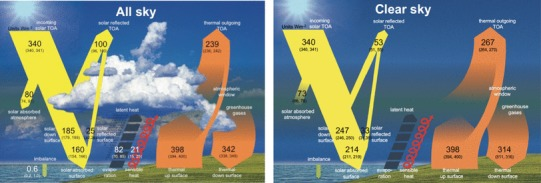
\includegraphics[scale = 7]{Chapter1_Intro/images/both_wild2019.jpg}
    \caption{The all-sky and the clear sky. Figure 14 Wild 2019. Ikke i bruk vennligst kommenter om denne er bedre enn den andre som viser differences mellom disse subplottene.}
    \label{fig:both_wild}
\end{figure}

Based on satellite and ground based measurements Wild et. al. 2019 \textbf{siter} have quantified the contribution of elements in the radiative budget. Subtracting the clear-sky from the all-sky climatology to compute the \acrfull{cre}. This is shown in equations \eqref{eq:cre_sw} and (\ref{eq:cre_lw}). Wild et. al. 2019 \textbf{siter} concludes with a reduction in shortwave radiation of $-47Wm^{-2}$ by clouds. In other words clouds reflect approximately 50\% of the incoming solar radiation. Longwave component is $28Wm^{-2}$. This give a net \acrshort{cre} of $-19Wm^{-2}$. Proving that the net effects of clouds on the radiative budget is negative.The altitude along with the composition determines the radiative properties of the cloud. \textbf{Relate this to the black body properties of clouds..? LES Artikkel fra Jonah}
\begin{figure}[h]
    \centering
    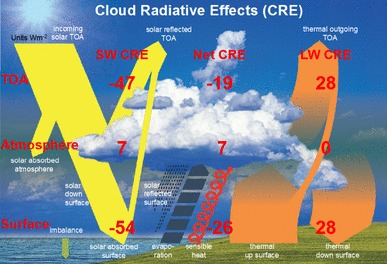
\includegraphics[scale = 7]{Chapter1_Intro/images/CRE_wild2019.jpg}
    \caption{Cloud radiative effect, CRE is the differece between the radiative components of the Clear sky radiative and the all sky. Cite this figure as fig 15 in Wild 2019}
    \label{fig:cre}
\end{figure}

\begin{equation} \label{eq:cre_sw}
    CRE_{sw} = SW\uparrow_{clear-sky} - SW\uparrow_{all-sky}
\end{equation}
\begin{equation} \label{eq:cre_lw}
    CRE_{lw} = LW\uparrow_{clear-sky} - LW\uparrow_{all-sky}
\end{equation}

The physical properties causing the interaction with radiation is described below. Dense low level clouds reflect solar radiation. This is called the albedo effect. Albedo being the ratio between reflected to incoming radiation. The higher number concentrations of droplets in a cloud the higher the total surface area of droplets. The more radiation gets reflected back into space. Clouds absorb longwave radiation and re-emits it. The absorbed radiation originates from the surface and is given by Stefan-Boltzmann forth-power law, see equation (\ref{eq:stefan-boltzmann}). The emmisivity, $\epsilon$ depends on the (composition, compactness and surface roughness) of the medium. Water, snow and ice have different spectral emmisivity. Huang et. al., 2018. Different parts of the globe are covered by different surfaces and Huang et al 2016 proved that assuming a constant suface emmisivity effects effects the TOA polar enegy buget. High clouds have low temperatures and since the re-emitted flux is a function of the cloud temperature. The greenhouse effect increases with the cloud altitude.
\textbf{Fokuser på at uavhengig av emmisiviteten til et medium er deet en funksjon av the fourth power of $T_{skin}$}

\begin{equation} \label{eq:stefan-boltzmann}
    F = \sigma \epsilon T ^4
\end{equation}

\section{Clouds in future climates} \label{sec:intro_cloud_future_climates}
\begin{figure}[h]
    \centering
    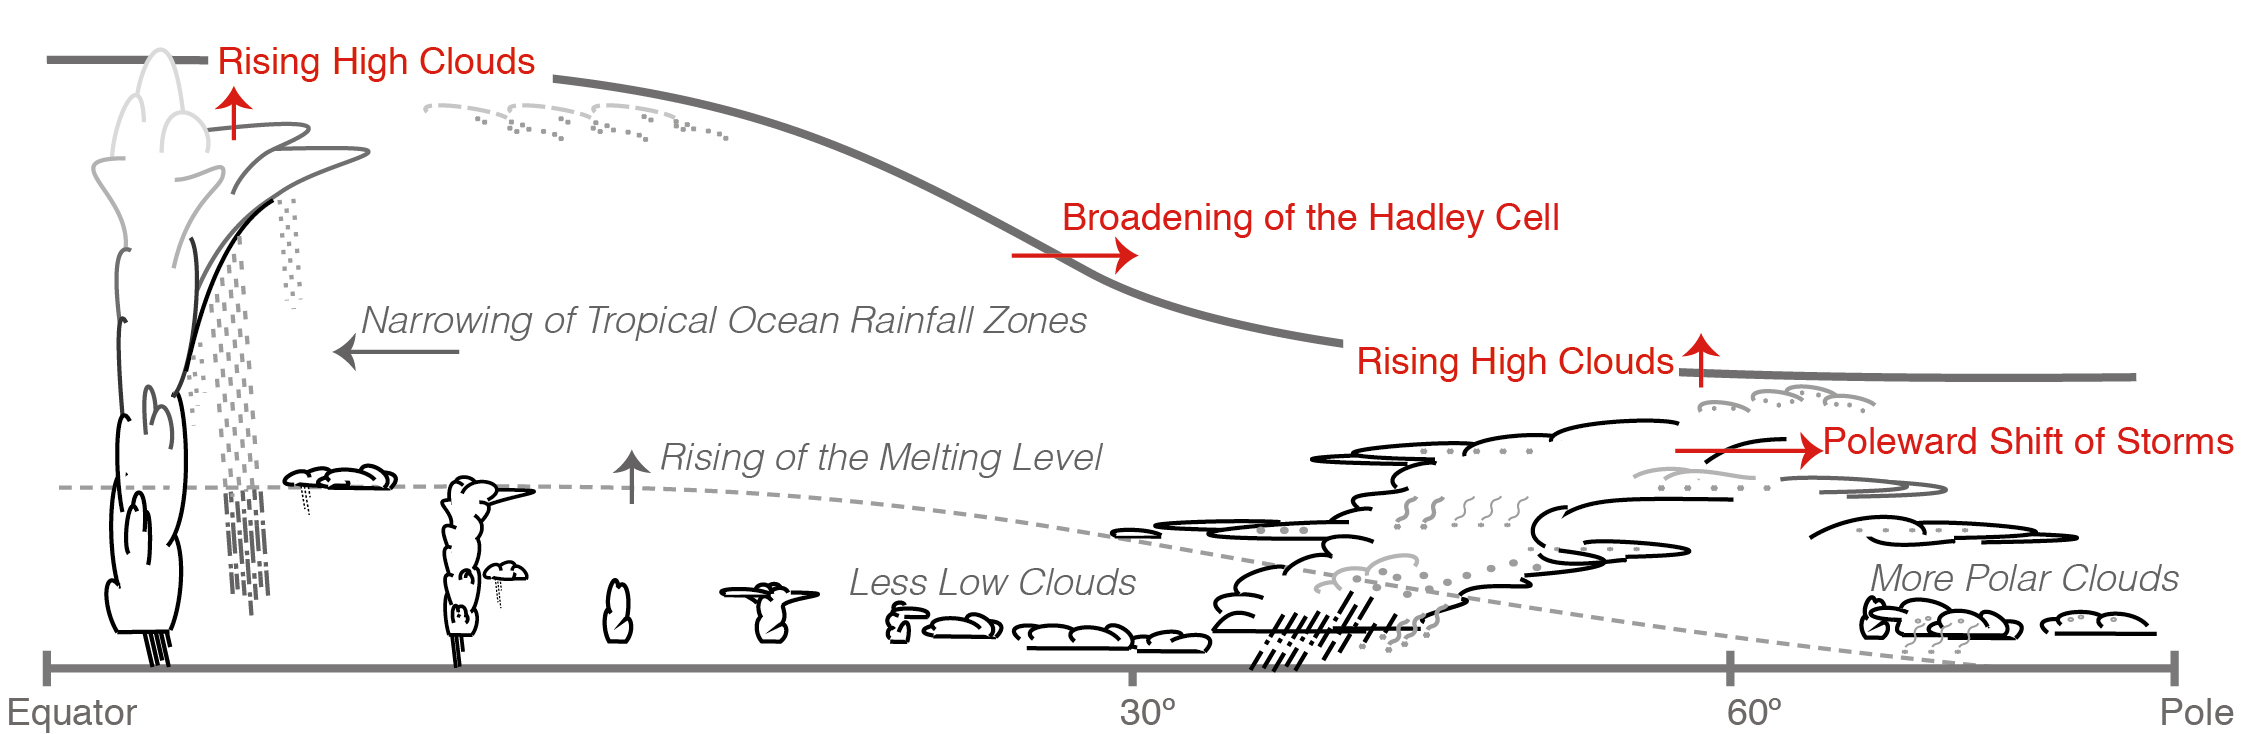
\includegraphics[scale = 0.8]{Chapter1_Intro/images/Fig7-11_ipcc.jpg}
    \caption{Cloud climatology in future climate. Developed based feedbacks in climate models, the different adjustments have different sikkerhet. Cite the fifth assessment report IPCC report.}
    \label{fig:cloud_scheme}
\end{figure}

Wild et. al. 2019  \textbf{siter} finds a imbalance of $0.6W m^{-2}$. This heat gets trapped in the earth system, forcing the surface temperature to increase in order to close the radiative budget. The imbalance in the radiative budget at \acrshort{toa} is the radiative forcing. Climate drivers include both natural and antropogentic forcings. This can be everything from natural variability in the solar energy output, vulcanic eruptions and green house gas emisions. The overall goal is to compute the climate sensitivity/equilibrium temperature as a function of forcing. For different \acrfull{rcp} scenarios one get a different temperature increase.
\\ \\ 
The global temperature will keep rising until we have reached the equilibrium climate temperature. This temperature increase induces climate changes. The \acrshort{ipcc} suggest the following shift in cloud schemes (see figure \ref{fig:cloud_scheme}). Figure \ref{fig:cloud_scheme} shows a summary of the most likely cloud feedbacks. First, a broadening of the Hadley cell causes a poleward shift of storms. This dries up the subtropics and moistens the higher latitudes. The clouds move further into the polar night, decreasing the albedo effect. 
%The albedo effect decrease at higher latitude. Moving the dense clouds further into the polar night. %Only the greenhouse effect of theses clouds persist. 
The greenhouse effect of clouds still persist without sunlight leading to a net heating in the Arctic. Second, rising higher clouds causing a stronger greenhouse effect. Third, less low level clouds, this is assumed to be partly offset by a increase in the melting layer, leading to more opaque clouds. Rising of the meltlayer cause ice crystals to melt resulting in more opaque clouds. These have a higher albedo and reflect more sunlight. 
\\ \\
Aerosols can alter the cloud micro-physics and in terms alter the radiative properties of the cloud. A polluted cloud gets extra \acrshort{ccn}, this results in more smaller droplets, as they share the available liquid. This increases the total surface area of the droplets. Which again reflect more radiation and could led to a enhanced lifetime, since it takes longer for the droplets to reach precipitation size. %If it does, it might not since only one out of ten cloud precipitate. \textbf{cloud physics book} 
When clouds persipitate they clean the air by removing particles.
\\ \\
Cloud micro-physical processes are not yet fully understood. Along with the fact that clouds are formed a smaller scale then can be resolved in your average climate models. Parametrizations are used to include the contribution from the subgridscale processes to the mesoscale proceses (weather phenomenons) in climate models and in weather predictions in general. Over the last years this has gained more attention since its acknowleged as the largest contributor to the uncertainty in climate models. I'll get back to this in chapter \ref{ch:theoretical_back}.

\section{Deep Learning} \label{sec:intro_deep_learning}
\textbf{Må begynne noen mer gripende eksempler på hva machine learning kan gjøre.}
Artificial intelligence dates back to the fifties when pioneers start talking about \textit{automating task normally performed by humans}. Machine learning is a means to achieve artificial intelligence. The progress in the field follows a sigmoid curve. Slow increase at first, then really steep, before it slows down again (see figure \textbf{ref sigmoid activation func}). Over the years there have been several discoveries kick-starting the development in machine learning. The very first algorithm's include probabilistic modelling. Using the principles of statistics to analyse data. This includes Naive Bayes classifiers and logistic regression. Two algorithm's which predates computers and are still useful today. Three main bottlenecks of advances in AI is hardware, data and algorithm's. Internet continuous to provide large amounts of data from Wikipedia, Flicker (tagged images) and YouTube. Advances in computational powers, such as graphical processing units, GPU's \textit{provide a environment/platform to learn in/on}. These where originally develop for the gaming industry, but in 2007 they realised a interface called CUDA (2007) which allows for computing \textbf{find a up to date cost and flops (floating point operations per second)}. \textbf{siter Chollet bok}
\\ \\ 
For clarity, the deep in deep learning refer to the number of layers. Moving from shallow networks to deeper ones (more than 10) algorithmic advances in gradient propagation was needed. This includes activation functions, weight initialisation and optimisation schemes. I'll get back to that in section \ref{sec:intro_machine_learning}. Other advances like batch normalisation, depth wise separable convolutions attributed to the revolution of \acrshort{ai}. 
\begin{figure}[h]
    \centering
    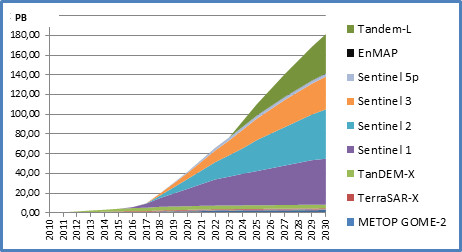
\includegraphics{Chapter1_Intro/images/Datenvolumen_D-SDA.jpg}
    \caption{Data volume. By the continuous earth system monitoring, meteorology/ climate science have progressed toward becoming a big data science. Observations are most used for verifying climate models and quantifying the current state of climate. \href{https://www.dlr.de/eoc/en/desktopdefault.aspx/tabid-12632/22039_read-51751}{https://www.dlr.de/eoc/en/desktopdefault.aspx/tabid-12632/22039{\_}read-51751}.}
    \label{fig:data_volum_sat}
\end{figure}
Earth system monitoring provides a global view of variables across meteorological systems. \textbf{Some thing about satellite era}. These large amounts of data and the flexible nature of the neural network makes is a suitable method also in geosciences. \textbf{With enough data neural networks can serve as a universal function approximate given a suitable hyper parameter tuning and input data.} The last couple of years reaserchers have been attempting to use this for wide range of problems like rainfall runoff modeling (krazerts), high-resolution weather forecasting (Rodrigues), Air quality forecasting (sun and liu), precipitaiton nowcastng (Shi et al) and \textbf{kanskje: LES} \textit{deep neural network based feature representation for weather data.} \textbf{lui et al }. \textbf{noe med forskjellig hell.} Another more comprehensive machine learning project is lead by Tapio Schneider at Caltech. Along with his team og technologist they have ambitions to create a earth system model using machine learning. With his team of from MIT and former employees of Microsoft and Google they hope to create a platform which can resolve clouds and hopefully reduce the spread in climate sensitivity. \textbf{cite Science}
\cleardoublepage

%\setcounter{chapter}{1} 
\chapter{Theoretical Background/ Climate and Cloud Physcis} \label{ch:theoretical_back}
This chapter describes the necessary theoretical background on clouds for this study. It is organised as follows. The three first sections describe the cloud's role in both present and future climate systems. Beginning with cloud formation and dissipation, including the cloud effects on Earth's radiative budget in the current climate and the suggestion of future cloud climatologies as proposed by \acrshort{ipcc} in \acrshort{ar5}. This is followed by a brief introduction to parameterization of clouds, i.e. the method used to incorporate clouds into climate models.
% Therefore necessary in studies of cloud feedback's. %in future climates. 
Finally, the data used in the compilation of the \acrshort{ecc} dataset is introduced. 

\section{Clouds role in the climate system} \label{sec:cloud_in_climate_system}
% Clouds, climate and machine learning
Clouds play an important role in the climate system. Both affecting the radiative budget and the hydrological cycle. Understanding how clouds form in the complex system of the atmosphere involves both knowledge about the large scale influence by the circulation and the small scale influenced by aerosols. Clouds are composed of liquid droplets, ice crystal or both. To this day the micro-physics of all phases are not fully understood. Here mixed phase clouds, consisting of both liquid and ice, shows to be the most difficult. 
%Climate models are the most useful tool for studying the past, present and future climate. Clouds and aerosols are acknowledged as the factors contributing with the largest uncertainty to the \acrfull{ecs}. Also known as global mean temperature increase as a consequence of doubling of the pre-industrial levels of $CO_2$ (280 \acrshort{ppm}). \textbf{kilde AR4 which ch?} \textit{It remains unclear to which level of sophistication is adequate to model their effect om climate.} (\cite{IPCC_CH7_clouds}).

%\textbf{Make sure you include everything that's related to parametrised processes.}
It is understood that cloud formation requires suitable aerosols and sufficient supersaturation. \textit{Aerosols} include both gases and solid particles suspended in air. They interact with the clouds by serving as particles which vapour and ice can condensate or deposit upon. The different phases require different properties and the nuclei are called \acrshort{ccn} for liquid droplets and \acrshort{inp} for ice crystals. Saturation is usually achieve by a temperature decrease in rising air masses. %Thus the stability of the atmosphere  plays a key role for convective motions.
%\textbf{Legg inn bilde a skyer en i is fase og en i liquids. Skriv noe som "the sharp outoline suggest that the cloud is consisting of liquid droplets, even at temperagtures below 0."}
%The negative temperature decreases by height is often referred to as the lapse rate, $\Gamma_{s, d}$. 
 
Growth processes are phase dependant. Liquid droplet grows by diffusion and later by collision and coalescence. At temperatures -38 $^oC$ (\cite{lohmann2016}) they will spontaneously freeze and could play the role as INP. 
%When both phases are present in a cloud, the saturation vapour pressure over ice is higher than over liquid. This may cause the droplets to evaporate and deposit on to the ice crystals. 
This mechanism exist because the saturation vapour pressure is lower with respect to ice than water. It is most efficient at 12$^oC$ when the difference is largest. This is called the Wegeron-Bergeron-Findeisen process. Clouds consisting purely of ice crystals first grow by deposition of vapour then by aggregation (\cite{Fowler1996LiquidAssumptions}). 

% Lots of different processes occurring simultaneously on different scales 
The complex nature of clouds originates from lots of different processes occurring simultaneously on different scales. Incorporating all these interactions into a model framework has proven to be difficult (\cite{IPCC_CH9_climate_models} +++ ). \textbf{Finn multiple sources} 

\section{Clouds in the current climate} \label{sec:intro_cloud_current_climate}
Based on satellite and ground based measurements \cite{Wild2019TheModels} have quantified the contribution of elements in the radiative budget. Cloud radiative effect (\acrshort{cre}) in earth annual mean energy budget between a cloudy and a cloud-free atmosphere. This is shown in equations \eqref{eq:cre_sw} and \eqref{eq:cre_lw}. \textbf{drop equations..?}
\cite{Wild2019TheModels} concludes with a reduction in shortwave radiation of $-47Wm^{-2}$ by clouds. In other words clouds reflect approximately 50\% of the incoming solar radiation. Longwave component is $28Wm^{-2}$. This give a net \acrshort{cre} of $-19Wm^{-2}$. Proving that the net effects of clouds on the radiative budget is negative.The altitude along with the composition determines the radiative properties of the cloud. 

\begin{figure}[h]
    \centering
    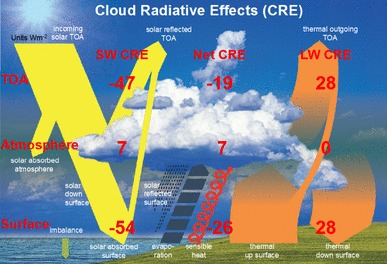
\includegraphics[scale = 7]{Chapter1_Intro/images/CRE_wild2019.jpg}
    \caption{Cloud radiative effect, CRE is the difference between the radiative components of the Clear sky radiative and the all sky. Modified version of as Figure 15 in \cite{Wild2019TheModels}. \textbf{pappa syns denne var grusomt vanskelig.}}
    \label{fig:cre}
\end{figure}

\begin{equation} \label{eq:cre_sw}
    CRE_{sw} = SW\uparrow_{clear-sky} - SW\uparrow_{all-sky}
\end{equation}

\begin{equation} \label{eq:cre_lw}
    CRE_{lw} = LW\uparrow_{clear-sky} - LW\uparrow_{all-sky}
\end{equation}

\begin{equation} \label{eq:stefan-boltzmann}
    F = \sigma \epsilon T ^4
\end{equation}

The physical properties causing the interaction with radiation is described below. Dense low level clouds reflect solar radiation. This is called the albedo effect. \textit{Albedo} being the ratio between reflected to incoming radiation. The higher number concentrations of droplets in a cloud the higher the total surface area of droplets. The more radiation gets reflected back into space. Clouds absorb longwave radiation and re-emits it. The absorbed radiation originates from the surface and is given by Stefan-Boltzmann forth-power law, see equation (\ref{eq:stefan-boltzmann}). The emissivity, $\epsilon$ depends on the (composition, compactness and surface roughness) of the medium. Water, snow and ice have different spectral emissivity (\cite{Huang2018ImprovedClimate}). Different parts of the globe are covered by different surfaces and \citeauthor{Huang2016AnSimulations} proved that assuming a constant surface emissivity effects the \acrshort{toa} polar energy budget. The greenhouse effect increases with the cloud altitude. Since high clouds have low temperatures and since the re-emitted radiation at a lower intensity than they absorbed. Researchers are still working on determine the emissivity of the different phases. Despite the uncertainties related to emissivity of the medium, the re-emitted radiation is of a lower intensity than what it absorb.

\section{Clouds in future climates} \label{sec:intro_cloud_future_climates}
\begin{figure}[h]
    \centering
    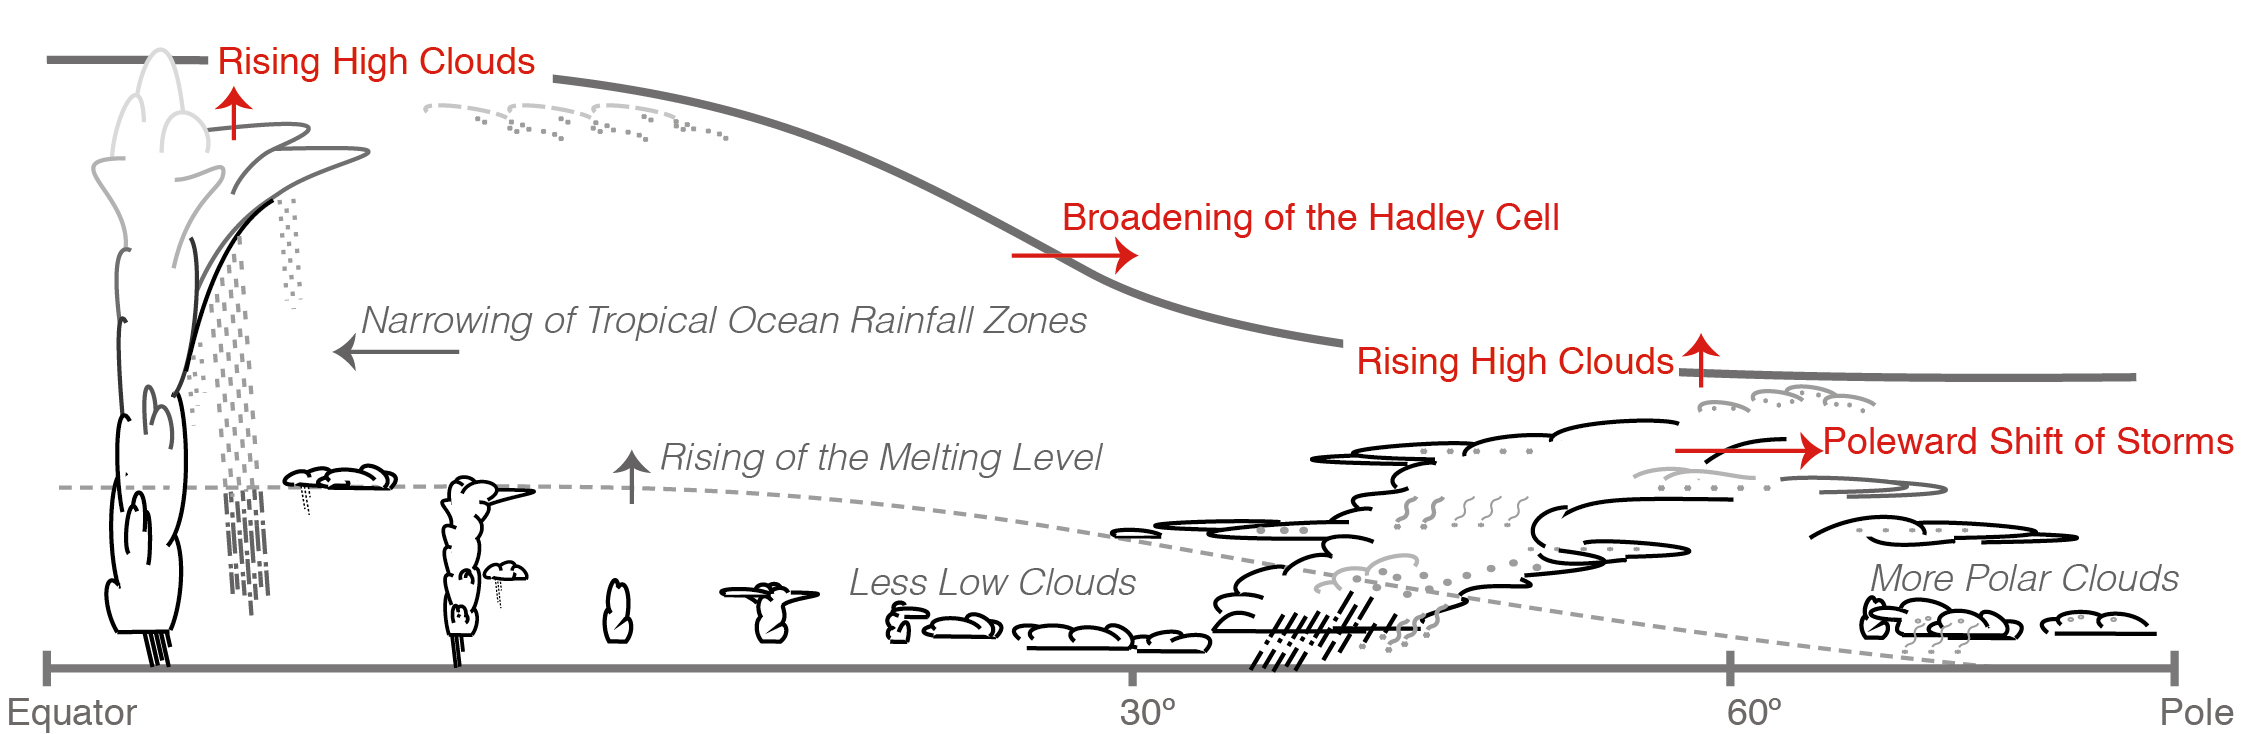
\includegraphics[scale = 0.8]{Chapter1_Intro/images/Fig7-11_ipcc.jpg}
    \caption{Cloud climatology in future climate. Developed based feedback's in climate models, the different adjustments have different uncertainty (\cite{IPCC_CH7_clouds}).}
    \label{fig:cloud_scheme}
\end{figure}

Excess of radiation gets trapped in the earth system, forcing the surface temperature to increase in order to close the radiative budget. The imbalance at the \acrfull{toa} is estimated by \cite{Wild2019TheModels} to be $0.6W m^{-2}$. 
% Wild et. al. 2019  \textbf{siter} finds an imbalance of This heat gets trapped in the earth system, forcing the surface temperature to increase in order to close the radiative budget. 
%The imbalance in the radiative budget at \acrfull{toa} is the radiative forcing. 
Climate drivers include both natural and anthropogenic forcings. \textit{Forcings} can be everything from natural variability in the solar energy output, volcanic eruptions and greenhouse gas emissions. The climate science community works toward a common goal to determine the climate sensitivity as a function of forcing. Different socio-economic pathways result different \acrshort{ecs}. The temperature increase induces climate changes. The \acrfull{ipcc} (\cite{IPCC_CH7_clouds}) suggest the following shift in cloud schemes (see figure \ref{fig:cloud_scheme}). Figure \ref{fig:cloud_scheme} shows a summary of the most likely cloud feedback's. First, a broadening of the Hadley cell causes a poleward shift of storms. This dries up the subtropics and moistens the higher latitudes. The clouds move further into the polar night, decreasing the albedo effect. The greenhouse effect of clouds still persist without sunlight leading to a net heating in the Arctic. Second, rising higher clouds causing a stronger greenhouse effect. Third, less low level clouds. This is assumed to be partly offset by a increase in the melting layer, leading to more opaque clouds. Rising of the meltlayer cause ice crystals to melt resulting in more opaque clouds. These opaque clouds have a higher albedo and reflect more sunlight. 
\section{Parametrization of clouds} \label{sec:param_clouds}
%\textit{In doing so, we do not include the effects of changes to the cloud microphysics explicitly.} Building a model based on meteorological variables provided by a reliable estimate from reanalysis datasets.
All global climate simulations are limited by computational power and the typical model grids are much too coarse to resolve all relevant processes governing clouds. Parameterization allows us to nevertheless simulate the effects of clouds on the climate, through simplified representations of cloud processes that are a function of resolved model variables. The development of both observational and modelling systems requires a understanding of the physical and biogeochemical processes that take place in the earth system (\cite{Simmons2016Observation2016-2025}). New ideas are implemented into models and tested. The simulated climate should be in accordance with observations and be able to recreate previous climate. 

The complex nature of clouds originates from lots of different processes occurring simultaneously on different scales. Incorporating all these interactions into a model framework has proven to be difficult (\cite{IPCC_CH9_climate_models}, \cite{IPCC_CH7_clouds} +++ ). \textbf{Finn multiple sources} 

% https://journals.ametsoc.org/doi/pdf/10.1175/2009JAS3072.1
% https://www.esrl.noaa.gov/psd/iasoa/vocabulary/Cloud%20Properties/Macrophysical
% Due to small scale of the processes involved, modelling the effects of clouds on the earth system requires parameterizations. 
% Due to the large uncertainty in \acrfull{ecs} related to clouds. 
%This area has received a lot of attention the last few years. A consequence of increasing the complexity of the models is the trailing increase in uncertainty. Popular approaches are saturation threshold, \acrfull{pdf} and \acrfull{crm}. 
%The data driven approach taken in this thesis does not net this case-specific adjustment. Doesn't need different approaches for different regimes, but relies on the satellites capabilities to detect them. Cirrus being the most difficult. When you one as seperate parameterizations for different cloud regimens, a consequence of this is that the cloud fraction might exceed 1.

\subsection{Relative humidity schemes}
The simplest form of cloud scheme is a binary. A model grid box is either cloudy or clear. Equation \eqref{eq:binary_param_clouds} describes a diagnostic relationship between cloud cover and relative humidity. Binary saturation threshold can be implemented as follows,
\begin{equation} \label{eq:binary_param_clouds}
    CFC\left(RH\right) = 
     \begin{cases}
       \text{0,} &\quad\text{if RH}\le100\\
       \text{1,} &\quad\text{else}
     \end{cases}
\end{equation}

\subsection{Statistical schemes}
Most climate models have a fractional cloud cover, which is driven by a saturation threshold. All the vapour in excess of this threshold, often $RH=100\%$, gets transformed into cloud liquid water. A representation of sub-grid scale variability is necessary to achieve fractional cloud cover. The most common variables either alone or in combination are relative humidity, temperature and vertical velocity (\cite{Golaz2002_part1}, ++ ).\textbf{cite more papers parametrizing this - draw inspiration from table?}  

Based on observations from airplane campaigns, researchers have attempted to draw statistical distributions of relevant variables. These \acrfull{pdf} are implemented into models. Virtually all existing \acrshort{pdf}s have been used to model either cloud cover or its dependent variables. % humidity, temperature and so on. 
%TS: Hva prøver du egentlig å si her over ("Virtually all...")? Jeg henger ikke helt med i resonnementet
A reproduction of the summary from \cite{Tompkins2009CloudParametrization}, describing distribution used in a selection of papers is given in Table \ref{tab:summary_PDF}.
\begin{table}[ht]
    \centering
    \setlength\tabcolsep{1.5pt} % default value: 6pt
    \setlength\extrarowheight{-7pt}
    \begin{tabular}{c|c|c}
        PDF shape &  Summary & Reference \\ \hline
        Double Delta & U, S & Ose (1993), Fowler et al. (1996) \\
        Uniform & U, S & LeTreut and Li (1991) \\
        Triangular & U, S & Smith (1990), Rotstayn (1997), Nishizawa (2000) \\
        Polynomial & U, S & Lohmann et al. (1999) \\
        Gaussian & U, S & Bougeault (1981), Ricard and Royer (1993) \\ 
        & &  Bechtolf et al. (1995) \\
        Beta & U, sk & Tomkins (2002) \\
        Log-normal & U, sk & Bony and Emanuel (2001) \\ 
        Exponential &  U, sk & Bougeault (1981), Ricard and Royer (1993) \\
        & &  Bechtolf et al. (1995) \\
        Double Gaussian/ Normal & B, sk & Lewellen and Yoh (1993), Golaz et al. (2002)
    \end{tabular}
    \caption{Reproduction of summary in \cite{Tompkins2009CloudParametrization}. Distributions used to parameterize cloud or its dependant variables. The key to decipher the summary column; U=Unimodal, B=Bimodal, S=Symmetric, sk = Skewed.}
    \label{tab:summary_PDF}
\end{table}
Researchers have not been successful in finding an adequate representation of cloud cover using these approaches (\cite{Tompkins2009CloudParametrization}). 

\cite{Golaz2002_part1} derived a joint \acrshort{pdf} of the sub-gridscale variability, serving as the base for parameterizing boundary layer clouds. This scheme is implemented in \acrfull{noresm} (\cite{SelandNORESM}) and \acrfull{cesm}, to recognised \acrshort{esm} (\cite{DanabasogluCESM}).
%TS: For NorESM kan du referere til Seland et al. (2002), og for CESM2 kan du referere til Danabasoglu et al. (2020)
The parameterization can be considered a higher-order turbulent closure problem. The first (mean), second (variance) and third order statistical moments, of the vertical velocity ($w$), the liquid water potential temperature ($\theta_l$), and the total water specific humidity ($q_t$) determines the family of \acrshort{pdf}s. It is designed to be flexible enough to (avoid the use of) circumvent the case specific adjustment. For more details see \cite{Golaz2002_part1} and \cite{Golaz2002_part2}.

%What is necessary to understand why clouds are Parameterisations. Cite that all climate models are wrong but some are useful.
\subsection{Cloud resolving models} \label{sec:params_climate_models}
Another method of cloud parameterization is using \acrfull{crm} that are integrated into global climate models. Contrary to what the name implies, this type of model still has problems with resolving the very smallest cloud processes, occurring on micrometer-scales. 

Running an \acrfull{les}-model, the increased resolution is able to resolve convective motions, but microphysical processes and turbulence effects still require parameterizations. \citeauthor{Baba2019SpectralModel} used this approach for parameterizing a spectral cumulus cloud. Obtaining the entrainment rate based on cloud properties from a \acrshort{crm} they built a parameterization valid for both shallow and deep convection. \textit{Entrainment rate} is the rate at which surrounding air penetrates the cloud. Preserving the physical properties, it is important that the method handles co-existing phenomena (\cite{Baba2019SpectralModel}). 

%Accelerating the speed of computations is always useful. 
\acrshort{dl} provides suitable methods for emulating %emulating what?, 
aimed to accelerate the speed of the heavy computations in \acrshort{crm}. Emulation in the context of computing refers to imitation of one model using another one. In this example the statistical models are used to mimic the behavior of the physically based \acrshort{crm}. The \acrshort{dl} model performance is restricted by the  \acrshort{crm}, performing at best as good as the \acrshort{crm} (\cite{Rasp2018DeepModels}).


\section{Data}
This section presents the data used in the compilation of the dataset, including background information about remote sensing of cloud properties and the method used to retrieve the data. 

\subsection{Summary reanalysis} \label{sec:summary_reanalysis}
\cite{Fujiwara2017IntroductionSystems}

\subsection{ERA5} \label{sec:era5}
ERA5 is the latest in the series of reanalyses produced by \acrfull{ecmwf}. Reanalysis is as close to observations as one can get while still obtaining data that is complete and coherent in both space and time. It is produced using a forecast model to assimilate observations. Data assimilation take observations as input and tries to make an accurate estimate of the state of the system that is as consistent as possible with the available observations at all times. This includes observations retrieved from satellites, ships, buoys, airplanes and ground-based stations. The analysis is produced in the operational forecast system, making it available within five days of real time. ERA5 is based on the Integrated Forecasting System, IFS cycle 4lr2. The data is available at a horizontal resolution of $0.25^o$ degree and hourly temporal resolution. It is an important product for the continuous monitoring of the Earth system 
(\cite{Hersbach2018OperationalStatus}).

Reanalyses data is often mistakenly referred to as observations. \citeauthor{Parker2016ReanalysesDifference} published an essay in \acrfull{bams} on this topic in \citeyear{Parker2016ReanalysesDifference}. Based on the following three points they conclude that observations and reanalyses are not too different. First, both involve inference, in other words, theory-based calculations. Second, reanalysis relies on forecast and observations do not. This is not a significant difference as long as the forecast is sufficiently accurate. Third, it is important to be aware that the uncertainty of the reanalyses is less well known than for observations. This makes it harder to judge the appropriate use of the reanalyses (\cite{Parker2016ReanalysesDifference}). 

\subsection{Remote sensing of cloud properties}
Satellites are the only instruments capable of providing continuous global measurements.
Measurements are collected by sensors, of which two types exist; passive and active imagers. The passive imaging sensors detect natural occurring levels of radiation, e.g. thermal radiation emitted by mediums. In contrast, active sensors  detect radiation returned from an emitted artificially fixed pulse of radiation (\cite{Stephens2018CloudsatSystem}). From \cite{Stockli2019CloudApplications}, \textit{the separation of the cloud from the cloud-free (reference signal) has been an everlasting problem in satellite-based cloud detection}.
\begin{figure*}
        \centering
        \begin{subfigure}[b]{0.475\textwidth}
            \centering
            \includegraphics[width=\textwidth]{Chapter2_Theory/images/sat_channels/meteosat-msg_wv062_overlay-ne_10m_coastline_overlay-ne_10m_admin_0_boundary_lines_land.png}
            \caption[Channel WV 6.2]%
            {{\small Channel WV 6.2}}    
            \label{fig:WV_6.2}
        \end{subfigure}
        \hfill
        \begin{subfigure}[b]{0.475\textwidth}  
            \centering 
            \includegraphics[width=\textwidth]{Chapter2_Theory/images/sat_channels/meteosat-msg_vis006_overlay-ne_10m_coastline_overlay-ne_10m_admin_0_boundary_lines_land.png}
            \caption[]%
            {{\small VIS 0.6}}    
            \label{fig:VIS_0.6}
        \end{subfigure}
        \vskip\baselineskip
        \begin{subfigure}[b]{0.475\textwidth}   
            \centering 
            \includegraphics[width=\textwidth]{Chapter2_Theory/images/sat_channels/meteosat-msg_ir108_overlay-ne_10m_coastline_overlay-ne_10m_admin_0_boundary_lines_land.png}
            \caption[something]%
            {{\small IR 10.8}}    
            \label{fig:IR_10.8}
        \end{subfigure}
        \quad
        \begin{subfigure}[b]{0.475\textwidth}   
            \centering 
            \includegraphics[width=\textwidth]{Chapter2_Theory/images/sat_channels/meteosat-msg_ir039_overlay-ne_10m_coastline_overlay-ne_10m_admin_0_boundary_lines_land.png}
            \caption{{\small IR 3.9}}    
            \label{fig:IR_3.9}
        \end{subfigure}
        \caption{{Spectral bands from SEVIRI. February 15th 2020 at noon. It shows the lowpressure system \textit{Elsa} positioned of the west coast of Iceland. Having a record breaking low of 915hPa (\cite{nrk_lavtrykk}). 
        The images are provided by  \cite{eumetcast_image_gallery}.}
    } 
    \label{fig:SEVIRI_channels}
\end{figure*}

% Info på bildene \textbf{Rectified (level 1.5) Meteosat SEVIRI image data. The data is transmitted as High Rate transmissions in 12 spectral channels. Level 1.5 image data corresponds to the geolocated and radiometrically pre-processed image data, ready for further processing, e.g. the extraction of meteorological products. Any spacecraft specific effects have been removed, and in particular, linearisation and equalisation of the image radiometry has been performed for all SEVIRI channels. The on-board blackbody data has been processed. Both radiometric and geometric quality control information is included. Images are made available with different timeliness according to their latency: quarter-hourly images if latency is more than 3 hours and hourly images if latency is less than 3 hours (for a total of 87 images per day). To enhance the perception for areas which are on the night side of the Earth a different mapping with increased contrast is applied for IR3.9 product. The greyscale mapping is based on the EBBT which allows to map the ranges 200 K to 300 K for the night and 250 K to 330 K for the day.}
% Lastet ned 16.02.2020.

\citepaper{Karlsson2015AdvancingData} list the five key properties exploited in remote sensing of clouds using passive imagery, these will be explained drawing examples from Figure \ref{fig:SEVIRI_channels}. High radiances are displayed in white and lower in darker colours. In general anything that appears bright has a higher reflection at the \acrshort{toa} than the surface. 

First, clouds appear bright as opposed to ice free water surfaces and vegetated Earth's surface in \acrshort{vis} and \acrshort{nir}. The detection from VIS 0.6 is shown in Figure \ref{fig:VIS_0.6}. Secondly, clouds consisting of liquid droplets reflect strongly in \acrfull{swir} and \acrfull{mwir}. The signal from MIR 3.9 is displayed in Figure \ref{fig:MIR_3.9}. Here the Earth's surface, including snow and ice, appear dark. Clouds are not perfectly emmiting black bodies and this allows for detection of low level clouds at night.

Another property exploited is that clouds are typically colder than the Earth's surface. Therefore they appear bright in IR channels, when displayed in reverse i.e. with low radiences shown as bright. 

The fourth property is that cirrus cloud are optically thin, but can be detected using split window channels (\acrshort{ir}10.8 and \acrshort{ir}12.0) differences (see Figure \ref{fig:IR_10.8}). The last property is not shown in this figure, but it is that in general broken clouds typically give rise to scattered patterns or texture in images with otherwise homogeneous, ice-free ocean for instance. 

Figure \ref{fig:WV_6.2} also show the signal detected from WV 6.2, water  vapour have a absorption band at these wavelength usefull for detected water vapour. 

To summarise, the success of a screening is dependent on the illumination, the state of the surface and atmosphere. And it has proven most difficult over bright surfaces like snow and dessert (\cite{Karlsson2015AdvancingData}). 

Improved technologies allow for measuring new variables, one example of such advances is the use of active sensors. Active sensors provide a more refined image of vertical profiles and allows for the detection of cloud phase. Despite the limitations of passive sensors they provide useful historical information and in some cases higher spatial and temporal resolutions. One attempt to relate passive measurements with active measurement under the same meteorological conditions is the \textit{Afternoon constellation, A-Train} launched as a cooperation between several space agencies; \acrfull{nasa}, \acrlong{jaxa} and the french \acrfull{cnes}. This has provided a useful link between the different types of measurements (\cite{Stephens2018CloudsatSystem}). 

The number of spectral bands and footprint size (pixel resolution) determine the practical application of a particular satellite retrieval. Differences in swath width determine the frequency at a given position, determining the temporal resolution. The viewing angle affects the optical properties of the medium, and also its apparent position. \textit{Parallax} describes the apparent shift in position of a object, caused by moving the observer along an axis. This is a known issue in remote sensing. Positions of satellites are changed. Moving the observer (satellite) changes the apparent position of the measurement. 
High viewing angles may cause similar issues, in detection of high clouds. This factor is negligible when detecting low clouds (\cite{Joro2010ComparisonFinland}). 

Differences in sensitivity and retrieval algorithms contribute to a large spread in global mean cloud amount among different cloud products. This also explains the difficulties involved in using one cloud dataset to evaluate another one. In their assessment of global cloud datasets \citepaper{Stubenrauch2013AssessmentPanel} compared the global mean cloud cover of six datasets (ISCCP, PATMOS-x, MODIS-ST, MODIS-CE, AIR-LMD and TOVS Path-B). In this process they eliminating MISR and ATSR-GRAPE because of different observation times (see Table 3 in \citepaper{Stubenrauch2013AssessmentPanel} ) and two outlier datasets, HIRS-NOAA and POLDER. Their results show that the difference among the six datasets is of order 0.08. In contrast, local differences could be up to 0.4 (\cite{Stubenrauch2013AssessmentPanel}). 

%%%%%%%%%%%%%%% NOTAT I TILFELLE JEG TENKTE JEG BURDE INKLUDERT FLERE DETALJER OM FLERE DATASET.
%Cloud-Aerosol Lidar and Infrared Pathfinder Satellite Observations, CALISO is much used in other research because it gives a vertically resolved cloud (3D observations). This additional spatial information is provided on the expense of frequency and uncertainty. \textit{Reason why calipso is ruled out as a candidate. large uncertainty Stubenau} MODIS has low spatial resolution but high temporal resolution, one to two days. National Oceanic and Atmospheric Administration, NOAA \textbf{ something}. Most polar orbiting satellites have a resolution at best daily. \textbf{kilde (shubenau)} \textbf{Does the other one give ferdig produkter av skyfraksjoner og eller er mye lettere og regridde??} The number of channels (higher for other than METEOSAT). The more channels you have the more accurate cloud detection algorihms you can use. Most of the uncertainty in satellite retrivals are attributed to the presence of clouds.  

\subsection{METeosat Second Generation, MSG} \label{sec:meteosat}
The \acrfull{msg} was established as a corporation between \acrfull{esa} and \acrfull{eumetsat}. \acrshort{esa} was in charge of developing the prototype of MSG-1. \acrshort{eumetsat} is responsible for maintaining the user requirements, launch procedures, developing ground segments, ensuring overall system consistency and day to day operations. 

The primary function of \acrshort{msg} is to provide continuous observations of the Earth's full disk. Near-constant sampling frequency and a geostationary orbit allows for observing weather phenomena occurring on short timescales. Located at $0^o$ \acrshort{msg} provides a varying spatial resolution, unlike the polar orbiting satellites. The resolution gets coarser with increasing off-nadir viewing angle (\cite{Stubenrauch2013AssessmentPanel}). %\textbf{This is a direct consequensce of the altitude the satellite needs to maintain in order to stay in geostationary orbit. DUPliCATED now}

There are efforts invested in extending the MSG dataset with the \acrfull{mfg}, in order to make use of the time series all the way back to 1980 (\cite{Bojanowski2018PerformanceGenerations}). This requires new cloud detection algorithms since they only have three common channels and only two of them are useful for detecting clouds (\cite{Stockli2019CloudApplications}). 
\begin{table}[]
    \centering
    \setlength\extrarowheight{-7pt}
    \begin{tabular}{c|c}
        Spectral band & Central wavelength $\left( \mu m  \right)$ \\ \hline
        VIS 0.6 & 0.635 \\
        VIS 0.8 & 0.81 \\
        NIR 1.6 & 1.64 \\
        IR 3.9 & 3.92 \\
        WV 6.2 & 6.25 \\
        WV 7.3 & 7.35 \\ 
        IR 8.7 & 8.7 \\
        IR 9.7 & 9.66 \\
        IR 10.8 & 10.8 \\
        IR 12.0 & 12 \\
        IR 13.4 & 13.4 \\
        HRV & 0.75
    \end{tabular}
    \caption{Summary of spectral bands, central wavelength and their respective retrieval abilities (\cite{Schmetz_meteosat_intro}).}
    \label{tab:msg_spectral_bands}
\end{table}

On board the \acrshort{msg} is the \acrfull{seviri} imaging radiometer. It has 12 spectral channels. The scan is done south to north, east to west. The wavelengths of the discrete channels are chosen based on heritage from other sensors. \arcshort{seviri} has one broadband visible channel, three solar channels (0.6, 0.8 and 1.6 $\mu m$) and 8 thermal infrared channels (3.9, 6.2, 7.3, 8.7, 9.7, 10.8, 12.0 and 13.4 $\mu m$) (\cite{Taravat2015MultilayerMasking}). Table \ref{tab:msg_spectral_bands}
 gives a summary of which properties is detectable by the different channels. 
This is of great advantage since much of the community already knows how to use the \acrshort{seviri} radiance observations. The channels have been chosen based on their ability to detect clouds, water vapour and ozone. More information about what the different channels detect is available in the paper \textit{An introduction to METeosat second generation (MSG)} published in \acrshort{bams} by \citepaper{Schmetz_meteosat_intro}.

Prior to the launch of the METeosat researchers discussed the temporal frequency suitable for observing weather phenomena. The METeosat first generation had a temporal resolution of 30min (\cite{Stockli2019CloudApplications}). For the second generation, 15min intervals were chosen to best cope with the short lifetime and rapid deformation of clouds. It was also suggested that a temporal frequency of 1 to 10min is necessary for tracking cumulus type clouds (\cite{Schmetz_meteosat_intro}). % 987 
This is in agreement with the Table 1.3 in \citeauthor{lohmann2016} (\citeyear{lohmann2016}, p. 19) stating the lifetimes of different types of clouds.

A \textit{ring} of geostationary satellites located at equator together provide global coverage (excluding polar regions). The altitude of the satellite determines its forward velocity. To achieve a geosynchronous orbit, a satellite needs to maintain a height of $\sim 36 000km$ (\cite{Bley2013ASEVIRI}). This height lead to a coarser spatial resolution than other satellite products retrived from other orbits. 

The first METeosat Second Generation (MSG-1) was launched 28 August 2002, and became operational 29 January 2004 when it was renamed METeosat-8. As a measure to reduce gaps, the \acrshort{msg} system provides a two-satellite system, one operational and one standby. The standby satellite scans when the operational satellite experiences technical failures. 
The operational satellite at nadir points at $0^o$ latitude. A full disk is $3712\times 3712$ pixels, and is sampled in cycles of 15min. This also include the on-board processing (\cite{Schmetz_meteosat_intro}).

\begin{figure}[h]
    \centering
    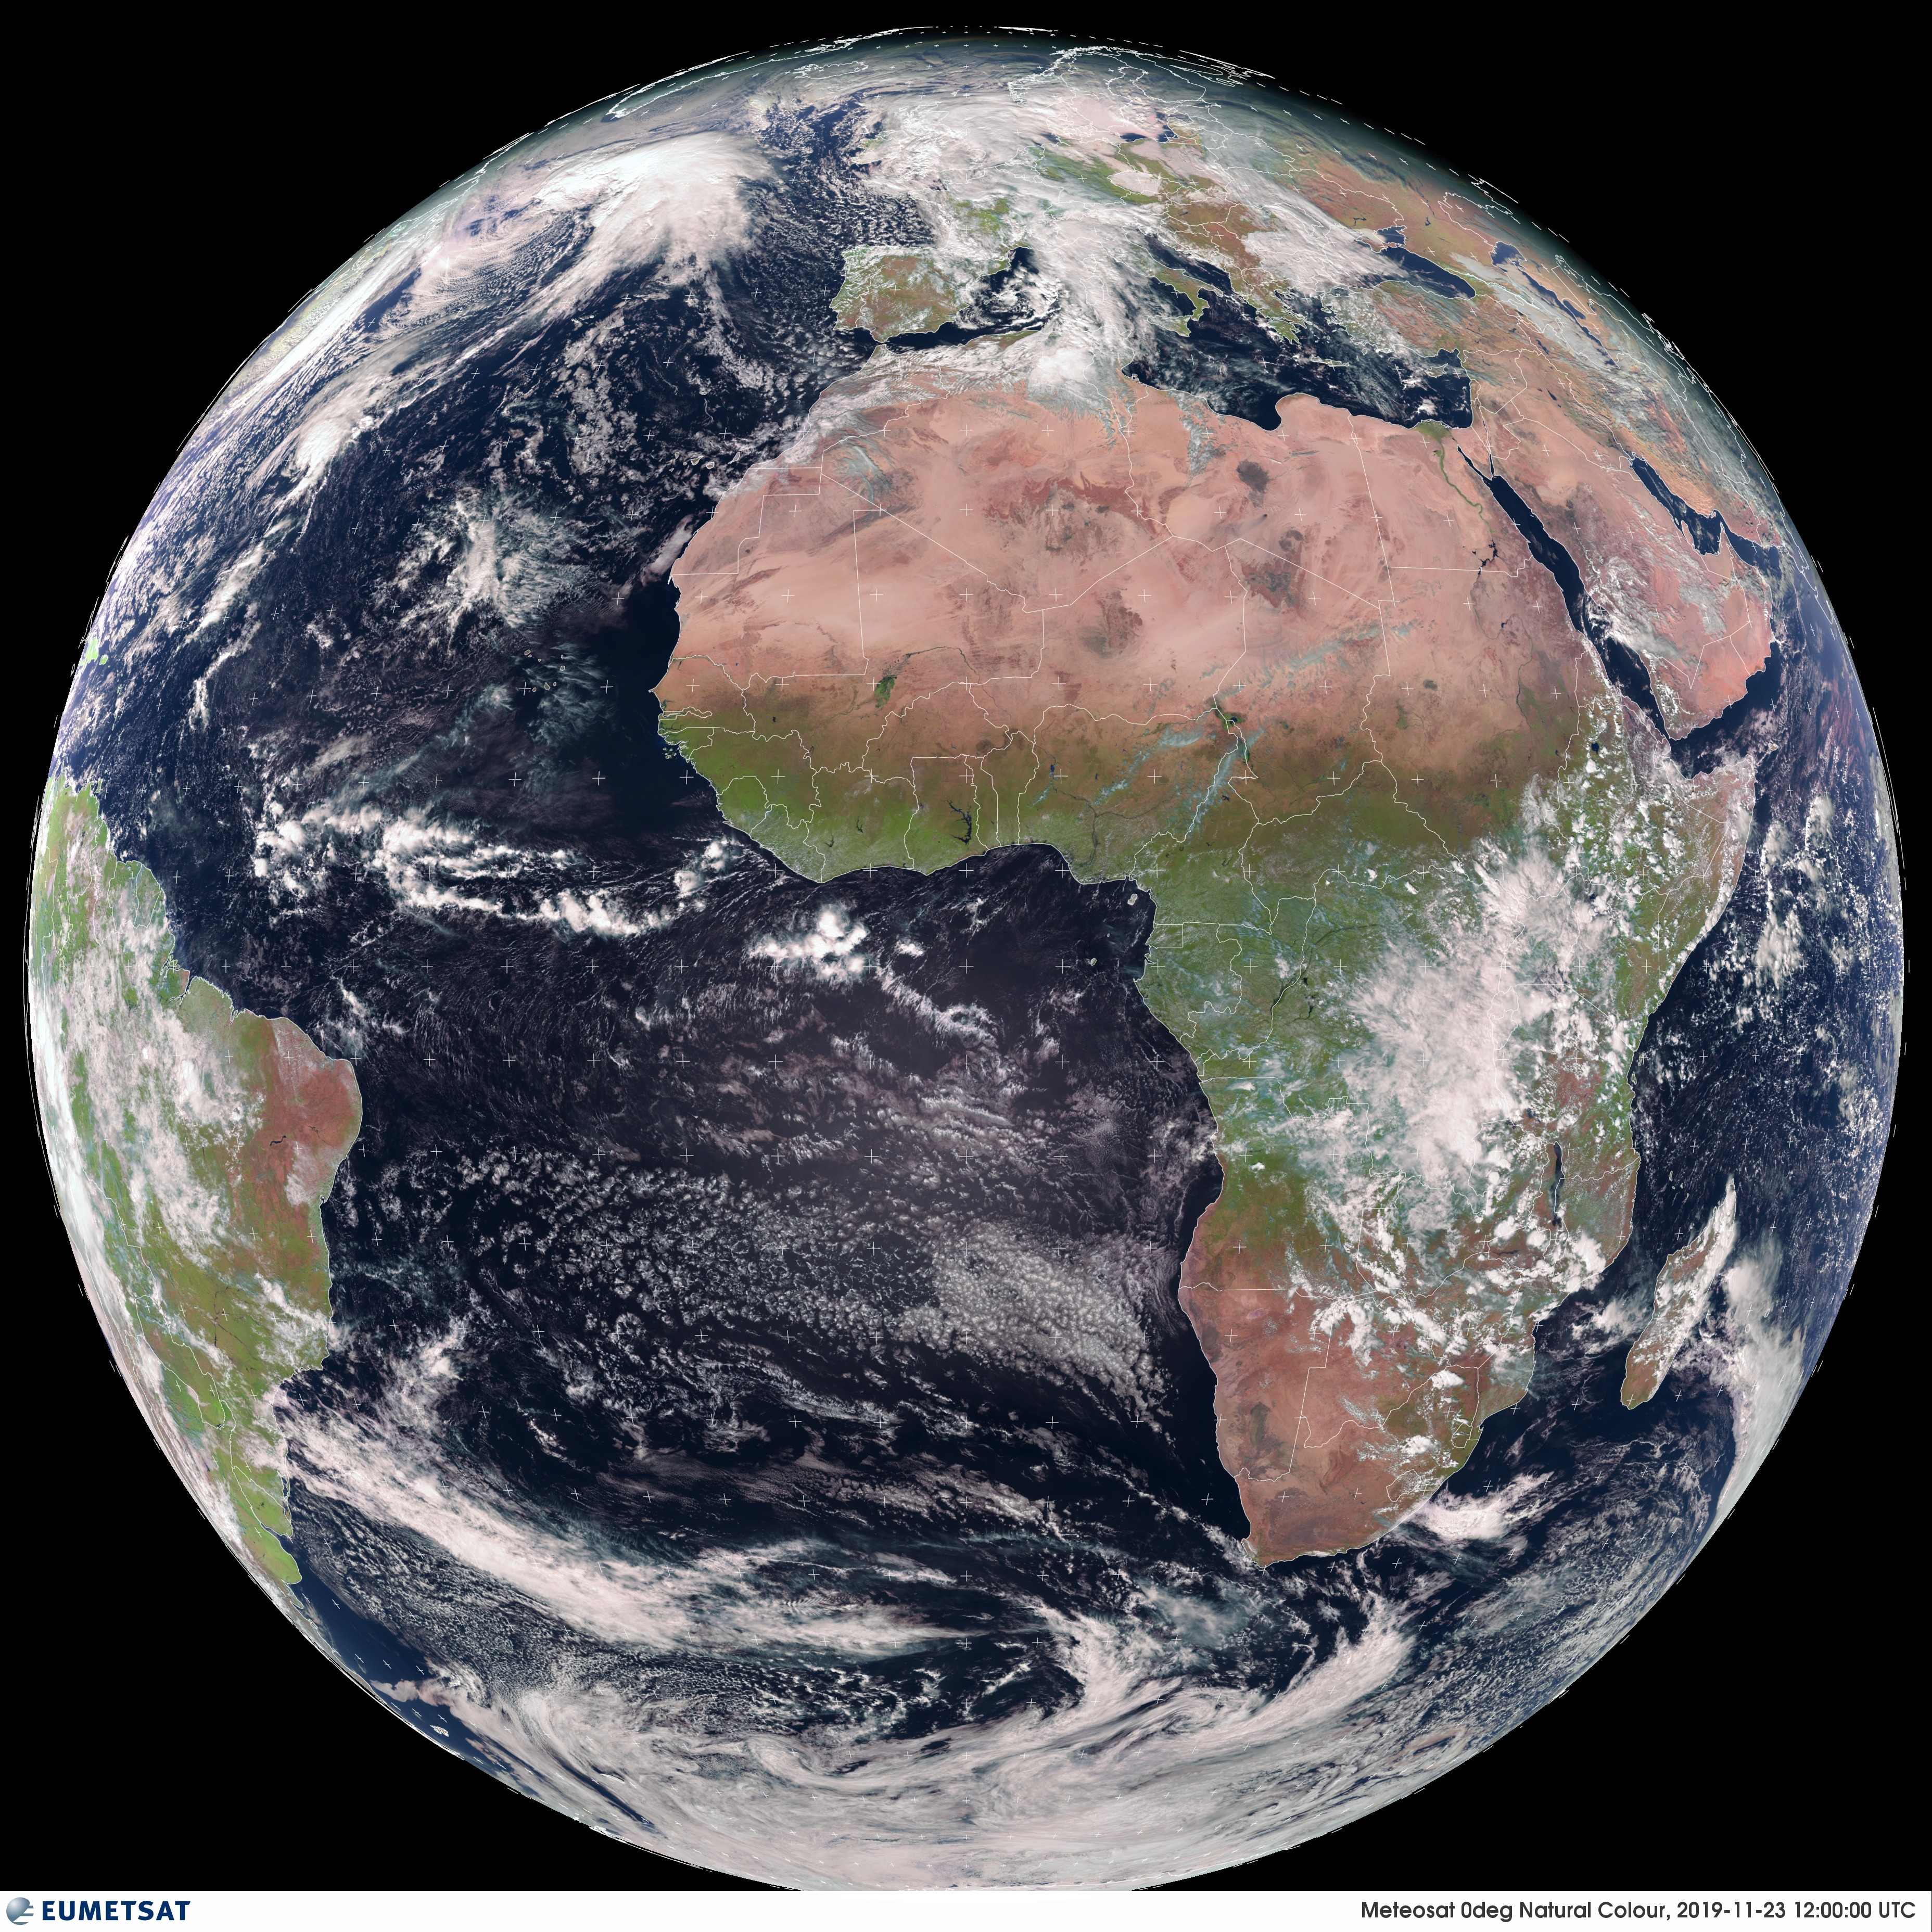
\includegraphics[scale=0.11]{Chapter2_Theory/images/MET10_RGBNatColourEnhncd_FullResolution_20191123120000.jpg}
    \caption{The view of Earth by \acrshort{seviri} on \acrshort{msg}, in naturally enhanced colours. This snapshot is dated noon 23rd of November 2019. By studying this image it becomes clear that clouds are influenced by circulation  (\cite{eumetcast_image_gallery}).}
    \label{fig:sat_view}
\end{figure}
The operational cloud detection algorithm is carried out pixel by pixel. Post processing involves re-classifying isolated pixels. There is a lot of effort invested in new detection algorithms including spatial structures. One of the methods that show potential here is deep learning (\cite{Dronner2018FastNetworks}, \cite{jeppesen_deep_cloud_masking}).

\subsection{EUMETSAT Cloud Mask} \label{sec:EUMETSAT_cloud_mask}
The \acrshort{eumetsat} cloud mask (CLM) consist of four classes, described in Table \ref{tab:classes_clm}.
\begin{table}[]
    \centering
    \setlength\extrarowheight{-7pt}
    \begin{tabular}{c|c}
        Class & Description \\ \hline
        0 & Clear sky over ocean \\
        1 & Clear sky over land \\
        2 & Cloudy \\
        3 & No data/ outer space        
    \end{tabular}
    \caption{Description of classes in EUMETSAT Cloud Mask product.}
    \label{tab:classes_clm}
\end{table}
These classes are derived from almost all channels except the broadband \acrfull{hrv} and isolated pixels are reclassified (\cite{Tavarat10_Derrien}). The cloud mask is distributed in \acrfull{grib},  without coordinates and \acrfull{netcdf}, processed with coordinates and reshaped into the standard rotation, as displayed i Figure \ref{fig:sat_view}. The data is available via Earth Observation Portal on \acrshort{eumetsat}'s web pages. 


\cleardoublepage

%%\setcounter{chapter}{2}
\chapter{Numerical Methods} \label{ch:num_methods}
This section introduce the computational methods used in generating the numerical experiments conducted in this thesis, starting with a short introduction to artificial intelligence. Followed by a brief introduction to the biological mechanisms the algorithms in this study draw inspiration from. This helps to gain insight to possible applications of different structures.
%Presenting the autoregressive model and convolutional long short-term memory. The performance metrics used to evaluate their performance and finishing of with automatic optimization routines.
% based on bio-inspired mechanisms are introduced
The task of forecasting in time and space requires two types of intelligence. One is computer vision, to understand the spatial relation and use the underlying physical properties. The other is sequential modelling to understand the temporal evolution.

Two approaches will be explored: Autoregressive models (AR) and Convolutional Long Short-Term Memory Network (ConvLSTM). The \acrshort{ar} model describes a time varying process, depending linearly on its previous values. The \acrshort{convlstm} approach is used to find a non-linear relation that describes phenomena varying in both time and space.
%Two approaches will be explored: autoregressive models (AR) and Convolutional Long Short-Term Memory Network (ConvLSTM). The AR model describes a time varying process, depending linearly on it previous values. The ConvLSTM is used to find a non-linear relation that describes phenomena varying in both time and space. %Another method used is the ConvLSTM.

The aim of this study is to determine whether the aggregation of linear models, or the more advanced non-linear model are better at prediction the complex phenomena varying in time and space.
%When used in tandem (all the linear models?), these models can predict complex natural phenomena ++++ .

%The popularity of \acrshort{dl} can be partly explained by its flexibility. This flexibility allows deep learning to be applied across many domains. The algorithms discussed here are simply a mathematical framework for learning model representations in data. The process of training is repeated until the network reaches an acceptable performance. In other words \textit{the extent to which this potential can be exploited is limited to the effectiveness of the training procedure applied} and also the data its provided. 

\section{Artificial Intelligence}
\begin{figure}[h] % h means place here if possible
    \centering
    \begin{tikzpicture}
        \draw [black, fill=orange, opacity = 0.3]  (2, -0.65) ellipse (2.5 and 1.25); % DL 
        \draw [black, fill=orange, opacity = 0.3]  (2, -0.25) ellipse (4 and 2); % ML
        \draw [black, fill=orange, opacity = 0.3]  (2, 0) ellipse (5.5 and 2.75);     % AI
        \node at ($(2, 2.125)$) {\Large Artificial Intelligence}; % +(2 and -0.65)
        \node at ($(2, 0.9)$) {\Large Machine Learning};
        \node at ($(2, -0.65)$) {\Large Deep Learning};
    \end{tikzpicture}
    \caption{Graph illustrating the subfields of \acrshort{ai}. \acrshort{ml} is a subfield of \acrshort{ai}, \acrshort{dl} is again a subfield of \acrshort{ml}. The sketch is inspired by Figure 1.1 in \citeauthor{chollet_book} (\citeyear{chollet_book}, p.5).}
    \label{fig:subcategories_AI}
\end{figure}
In encounters with geoscientists the author often get the question: \textit{What is the difference between machine learning and artificial intelligence?} The short answer is: they are not different fields, but \acrshort{ml} is a subfield of AI. Algorithms developing its own ``knowledge'' from supplied examples falls into the category of ML and not the base category of AI. ML is distinct in that it attempts to deduce rules and go beyond human intuition using a complex net of interactions. 

In fact, it is worth mentioning that there is a subfield of \acrshort{ml} known as \acrshort{dl} (see graph in Figure \ref{fig:subcategories_AI}). %Deep learning is a subfield of machine learning, making it a subfield of artificial intelligence. %Deep learning provide a improved. 
\acrshort{dl} is at the frontier of AI research, with many recent advances being made in this subfield. The popularity of \acrshort{dl} can be partly explained by its flexibility. This flexibility allows \acrshort{dl} to be applied across many domains. The algorithms discussed here are simply a mathematical framework for learning model representations in data. The process of training is repeated until the network reaches an acceptable performance. In other words, the potential is limited by the data and the effectiveness of the training procedure applied.

%The origin of the subfields has a historical explanation. Each subfield is linked to significant advances.%, which will be explained using parallels to the long standing problem of computer chess. 
\begin{figure}[h] % h means place here if possible
\centering
\def\layersep{2.5cm}
\begin{tikzpicture}[shorten >=1pt,->,draw=blue, node distance=\layersep]
    \tikzstyle{every pin edge}=[<-,shorten <=1pt]
    \tikzstyle{neuron}=[circle,fill=black!25,minimum size=17pt,inner sep=0pt]
    \tikzstyle{input neuron}=[neuron, fill=green];
    \tikzstyle{output neuron}=[neuron, fill=red];
    \tikzstyle{hidden neuron}=[neuron, fill=cyan];
    \tikzstyle{annot} = [text width=4em, text centered]

    \node[input neuron] (I-1) at (0,-1) {}; % {$T_{2m}$};
    \node[input neuron] (I-2) at (0,-2) {}; % {$q_v$};
    \node[input neuron] (I-3) at (0,-3) {}; % {$RH$};
    \node[input neuron] (I-4) at (0,-4) {}; % {$p_s$};

    % Draw the input layer nodes
    %\foreach \name / \y in {1,...,4}
    % This is the same as writing \foreach \name / \y in {1/1,2/2,3/3,4/4}
    %    \node[input neuron, pin=left:Input \#\y] (I-\name) at (0,-\y) {};

    % Draw the hidden layer nodes
    \foreach \name / \y in {1,...,5}
        \path[yshift=0.5cm]
            node[hidden neuron] (H-\name) at (\layersep,-\y cm) {};

    % Draw the output layer node
    \node[output neuron, right of=H-2] (O) {};
    \node[output neuron, right of=H-3] (O1) {};
    \node[output neuron, right of=H-4] (O2) {};


    % Connect every node in the input layer with every node in the
    % hidden layer.
    \foreach \source in {1,...,4}
        \foreach \dest in {1,...,5}
            \path (I-\source) edge (H-\dest);

    % Connect every node in the hidden layer with the output layer
    \foreach \source in {1,...,5}
        \path (H-\source) edge (O);
        %\path (H-\source) edge (o1);
        %\path (H-\source) edge (o2);

    % Does the same thing the loop does had to do it manually tho
    \path (H-1) edge (O1);
    \path (H-2) edge (O1);
    \path (H-3) edge (O1);
    \path (H-4) edge (O1);
    \path (H-5) edge (O1);
    
    \path (H-1) edge (O2);
    \path (H-2) edge (O2);
    \path (H-3) edge (O2);
    \path (H-4) edge (O2);
    \path (H-5) edge (O2);

    % Annotate the layers
    \node[annot,above of=H-1, node distance=1cm] (hl) {Hidden layer};
    \node[annot,left of=hl] {Input layer};
    \node[annot,right of=hl] {Output layer};
\end{tikzpicture}
\caption{Fully connected feed forward neural network with one hidden layer. The connections between the layers are the weights. The sketch is based on the example provided by \citepaper{ffnn}.}
\label{fig:one_layer_mlp}
\end{figure}
%The input layer has four units, the hidden layer has five and the output layer has three. In total there are 35 parameters in this network (37 if bias is included).
\acrshort{ai} in general and \acrshort{dl} in particular emerged from considerations of perception and cognition in biology. Many of the \acrshort{dl} network architectures draw inspiration from the human brain. The architecture of \acrshort{dl}, while distinct from biological computing, is named such that concepts in neuroscience and computing can be treated analogously. For example using building blocks such as nodes (artificial neurons), weights (connections between nodes), rules of signal propagation, activation (transfer function) and learning algorithms (training algorithms).

Figure \ref{fig:one_layer_mlp} illustrates a simple artificial neural network. The circles illustrate nodes (neurons). Nodes belonging to the same layer is shown in one colour. Arrows illustrates weights, the connections between the layers. It shows that nodes belonging to the same layer are not connected, but nodes in consecutive layers are connected with weights. 

%Figure \ref{fig:one_layer_mlp} illustrates a simple artificial neural network. Artificial intelligence (AI) in general and Deep Learning (DL) in particular emerged from biological inspired computing. Many of the DL network architectures draw inspiration from the human brain. The architecture of DL, while distinct from biological computing, is named such that concepts in neuroscience and computing can be treated analogously. For example using building blocks such as neurons (nodes, units), weights (connections between neurons), rules of signal propagation, activation (transfer function) and learning algorithms (training algorithms). % \textbf{Raymond: Må skille mellom AI og DL - AI er ikke nødvendigvis basert på en modell av hjernen.}
%The circles illustrate nodes (neurons). Nodes belonging to the same layer is shown in one color. Arrows illustrates weights, the connections between the layers. Nodes belonging to the same layer are not connected, but nodes in consecutive layers are connected with weights. 
% \textbf{cite \href{https://www.sciencedirect.com/topics/engineering/neural-network-architecture}{\textbf{https://www.sciencedirect.com/topics/engineering/neural-network-architecture}}}
Sequence modelling draws parallels to the human memory. This type of modelling requires information about earlier stages, retained in memory. Simple models have one memory centre. Drawing inspiration from the brain, other more complex models make the distinction between a short term and a long memory centre. Finishing sentences for others is a trivial task for humans. The reader should not be surprised by the following \textit{the clouds are in the \ldots sky} (\cite{colah_blog_post}).

AI started with the idea of automating tasks normally performed by humans. Three factors determine advances in the field of AI: data, hardware, and algorithms (\cite{chollet_book}). This explains why there often is a significant time gap between an idea and breakthroughs in the architectures and results. Convolution neural networks (CNN), for example, were conceptually developed in the 80s (\textbf{add citation}), but a lack of sufficient computing power (hardware) kept their use in hibernation until 2012, when a \acrshort{cnn} (AlexNet) won the ImageNet challenge, an image recognition contest (\cite{AlexNet}).

% Removed chess example..
% Computer chess is the longest studied problem in the history of artificial intelligence and advancements in computer chess provide good examples on the evolution of AI. In 1951, Alan Turing was the first to publish a program, on paper, capable of playing a entire game of chess. 
%\textbf{Første model for ANN (Artificial Neural Network) ble laget i 1943. ``Perceptron'' ble beskrevet i 1958, første multi-layer network publisert i 1965, ``continuous backpropagation'' ble utledet i 1960/1961, \ldots ANN/DL har altså en lang historie, i hovedsak drevet av forbedrede algoritmer, men det er først det siste tiåret at maskinvaren er blitt kraftig nok til at neuralnettverk, og da i første rekke ved hjelp av grafikkakseleratorer (GPU).}
%\textbf{Turing's sjakkprogram er vel strengt tatt heller et eksempel på ``Rule-Based AI''? Alle reglene var bestemt på forhånd, men programmet prøvde for hvert trekk å finne det beste alternativet ut fra tilstanden på brettet og hvilke muligheter motspilleren ville få i sitt neste trekk.}
% (leads into architecture paragraph)
%Starting with explicitly trained programs. This falls in the category of AI and not ML.
%\textit{Learning, in the context of ML, describes the automatic search for a better representations.} 
%The network is presented with many examples and is trained, rather than explicitly programmed. 
Geoscientists may be more familiar with the concept of ``calibration'' when it comes to statistical models, which essentially is the same process. In the context of deep learning, ``deep'' refers to the number of layers contributing to a network. DL expands the ideas from ML using deeper networks, \textit{i.e,} more layers, enabling networks to capturing a more complex relationship between input and output variables.
%\textbf{``e.g.'' betyr ``exempli gratia'', altså for eksempel; ``i.e.'' betyr ``id est'' -- ``det er'', ``altså''}
%\textbf{Michael is ``backpropagation'' one of the differences between ML and DL?}
%Geoscientists may be more familiar with the concept of "calibration" when it comes to statistical models, which essentially is the same process. In the context of deep learning, deep references to the number of layers contributing to a network, and thus the complexity of relationship between input variables. DL expands the ideas from ML using deeper network, e.g. more layers. 
\begin{figure}[h] % h means place here if possible
\centering
\def\layersep{2.5cm}
\begin{tikzpicture}[shorten >=1pt,->,draw=blue, node distance=\layersep]
    \tikzstyle{every pin edge}=[<-,shorten <=1pt]
    \tikzstyle{neuron}=[circle,fill=black!25,minimum size=17pt,inner sep=0pt]
    \tikzstyle{input neuron}=[neuron, fill=green];
    \tikzstyle{output neuron}=[neuron, fill=red];
    \tikzstyle{hidden neuron}=[neuron, fill=cyan];
    \tikzstyle{annot} = [text width=4em, text centered];

    % Determining the input layer.
    \node[input neuron] (I-1) at (0,-1) {}; % {$T_{2m}$};
    \node[input neuron] (I-2) at (0,-2) {}; % {$q_v$};
    \node[input neuron] (I-3) at (0,-3) {}; % {$RH$};
    \node[input neuron] (I-4) at (0,-4) {}; % {$p_s$};

    % Draw the input layer nodes
    %\foreach \name / \y in {1,...,4}
    % This is the same as writing \foreach \name / \y in {1/1,2/2,3/3,4/4}
    %    \node[input neuron, pin=left:Input \#\y] (I-\name) at (0,-\y) {};

    % Draw the hidden layer nodes
    \foreach \name / \y in {1,...,5}
        \path[yshift=0.5cm]
            node[hidden neuron] (H-\name) at (\layersep,-\y cm) {};

    % Connect every node in the input layer with every node in the
    % hidden layer.
    \foreach \source in {1,...,4}
        \foreach \dest in {1,...,5}
            \path (I-\source) edge (H-\dest);

    % Draw the hidden layer nodes
    \foreach \name / \y in {1,...,5}
        \path[yshift=0.5cm]
            node[hidden neuron] (R-\name) at (2*\layersep,-\y cm) {};

    % Connect every node in the input layer with every node in the
    % hidden layer.
    \foreach \source in {1,...,5}
        \foreach \dest in {1,...,5}
            \path (H-\source) edge (R-\dest);

    % Draw the hidden layer nodes
    %\foreach \name / \y in {1,...,5}
    %    \path[yshift=0.5cm]
    %        node[hidden neuron] (T-\name) at (3*\layersep,-\y cm) {};

    % Draw the hidden layer nodes
    \foreach \name / \y in {1,...,5}
        \path[yshift=0.5cm]
            node[hidden neuron] (L-\name) at (4*\layersep,-\y cm) {};

    % Connect every node in the input layer with every node in the
    % hidden layer.
    \foreach \source in {1,...,5}
        \foreach \dest in {1,...,5}
            \path[dashed] (R-\source) edge (L-\dest);



    % Connect every node in the input layer with every node in the
    % hidden layer.
    %\foreach \source in {1,...,5}
    %    \foreach \dest in {1,...,5}
    %        \path (R-\source) edge (T-\dest);



    % Draw the output layer node
    \node[output neuron, right of=L-2] (o1) {};
    \node[output neuron, right of=L-3] (o2) {};
    \node[output neuron, right of=L-4] (o3) {};

    % Connect every node in the hidden layer with the output layer
    \foreach \source in {1,...,5}
        \foreach \dest in {1,...,3}
            \path (L-\source) edge (o\dest);

    % Annotate the layers
    \node[annot,above of=H-1, node distance=1cm] (hl) {Hidden layer};
    \node[annot,above of=R-1, node distance=1cm] (hr) {Hidden layer};
    %\node[annot,above of=T-1, node distance=1cm] (ht) {Hidden layer};
    \node[annot,above of=L-1, node distance=1cm] (hL) {Hidden layer};

    \node[annot,left of=hl] {Input layer};
    \node[annot,right of=hL] {Output layer};
\end{tikzpicture}

\caption{Deep fully connected neural network. The sketch is based on the example by \cite{ffnn}.}
\label{fig:multilayer_mlp}
\end{figure}
Figure \ref{fig:multilayer_mlp} illustrates a deeper version of the network displayed in Figure \ref{fig:one_layer_mlp}. A layer is a set of nodes. The connections between the layers are the trained units, also known as weights. 

To distinguish from deep learning, traditional \acrshort{ml} is sometimes referred to as shallow learning. Linear regression (LR) is a ML algorithm predating computers which is still useful today. Traditional LR can be derived using shallow learning methods. 
\textbf{Hugo: ML three categories: 1) Methods that are not based on artificial neural networks such as linear regression models and other regression models, decision trees, random forest, support vector machine etc 2) Artificial neural networks with few layers (shallow) and generally few parameters. 3) Artificial neural networks with many layers and a lot of parameters in each layer (deep learning)}

``Intelligence'', in the context of artificial intelligence, is still a topic of debate. Traditionally, a machine would be considered intelligent if it could beat a human at a given task (\cite{Chollet2019OnIntelligence}). For computer chess, this was achieved in 1997 when IBM's DeepBlue beat Gary Karsparov. Researchers had learned how to build a ``rule-based'' chess-playing AI, but not a program that could generalize to anything beyond similar boardgames. In retrospect, scientists have realized that most architectures are not well matched to human intelligence. 
%\textbf{Raymond: DeepBlue var i hovedsak regel-basert, men Google's AlphaZero er (delvis) basert på DL.}
%See the paper from to get more information about the specifics \textbf{cite paper}. Based on studies in psychology, it is clear that the game of chess involves complex reasoning, search, perceptual and memorial processes. While one can solve chess using these abilities, one can also solve chess by taking radical shortcuts, that the human mind is not capable of. 
% Explain glossaries or words that are used a lot.
%Intelligence, in the context of artificial intelligence, is still a topic of debate. Traditionally, a machine would be considered intelligent if it would beat a human at a given task. For computer chess, this was achieved in 1997 when IBM's DeepBlue beat Gary Karsparov. Researchers had learned how to build a chess-playing AI, but not a program that could generalize to anything beyond similar boardgames. In retrospect, scientist have realized that this particular architecture is not be informative on human intelligence. See the paper from to get more information about the specifics \textbf{cite paper}. Based phsycology studies its clear that the game of chess involves complex reasoning, search, perceptual and memorial processes. While one can solve chess using these abilities, one can also solve chess by taking radical shortcuts, the human mind is not capable of. 
%Researchers became aware that they had learned less to nothing about how the human mind works. The original understanding of machine intelligence has been abandoned in search for a more complete definition. \textbf{chollet google artikkel}

There are several different types of machine learning, each suitable for solving different tasks. Figure \ref{fig:machine_learning_categories} shows the types of ML and their subcategories. These subcategories also exist for deep learning, the only difference being the number of layers used.
%, but in order to keep this as general they are described from the above level. Keep in mind that their deep learning cousins can be referred to by simply adding the prefix 'deep'. 
% Example on deep reinforcement learning.
%The frontier of chess playing programs is AlphaZero. The deep reinforcement learning architecture trained is using self-play. Without having any previous knowledge of rules. 

%Supervised learning is the part of machine learning concerned with learning the relation between input data, x and labelled data, y. Regression predict continuous values. Replicating a function. Classification is discrete, since it assigns a category to the input. 
%Reinforcement learning is a goal-oriented algorithms, most known for playing chess, solving labyrinths and lately \textcolor{red}{for?} active flow control \textbf{Cite Jean Rau, three papers}. \textcolor{red}{(Nytt avsnitt?)} 
%Unsupervised learning tries to detect patterns in unlabelled data. This includes clustering and dimensionality reduction. Dimensionality reduction has been used by climatologist for decades in order to remove seasonal variation \textbf{cite Benestad}. Unsupervised and reinforcement learning is out of the scope of this thesis and will not be discussed further.
%author : Hanna Svennevik
\begin{figure}[hp]
    \centering
    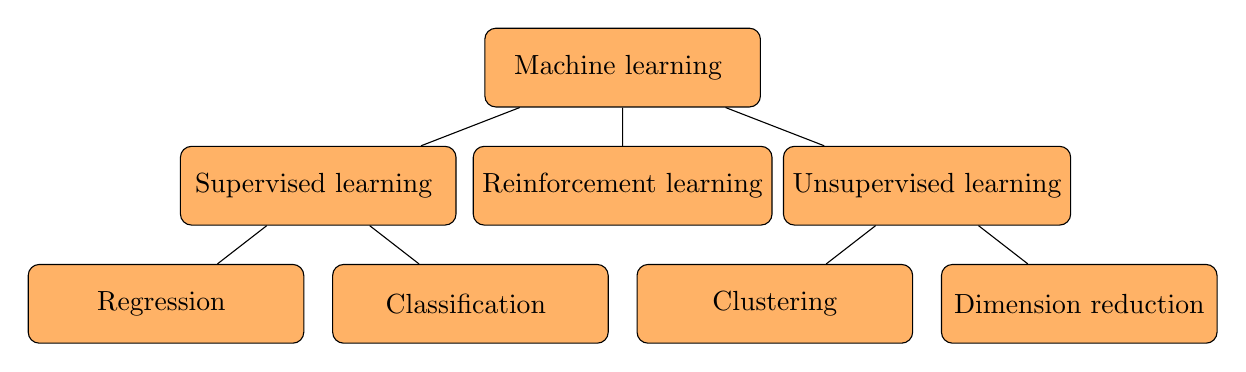
\begin{tikzpicture}[sibling distance=11em,
  every node/.style = {shape=rectangle, rounded corners,
    draw, align=center, 
    %top color=white, bottom color=cyan!20,
    fill=orange!60, minimum width=3.5cm, minimum height = 1.0cm}]]
  \node { Machine learning }
    child { node {  Supervised learning  } 
        child { node {  Regression   } }
        child { node {  Classification  } }
    }
    child {node {Reinforcement  learning}}
    child {node {Unsupervised learning}
           child { node {Clustering}}
           child { node {Dimension reduction}}};
\end{tikzpicture}
    \caption{The graph shows the different type of machine learning and their subcategories.}
    \label{fig:machine_learning_categories}
\end{figure} 

\begin{itemize}
    \item \textbf{Supervised learning}: part of machine learning concerned with learning the relation between input data, x and labelled data, y.
    \begin{itemize}
        \item Regression\\predict continuous values. Replicating a function.
        \item Classification\\discrete, since it assigns a category to the input.
    \end{itemize}
    \item \textbf{Unsupervised learning}: Detecting patterns in unlabeled data.
    \begin{itemize}
        \item Clustering\\Grouping a set of data points into a predescribed number of groups
        \item Dimension reduction\\Reducing the number of random variables under consideration.
    \end{itemize}
    \item \textbf{Reinforcement learning}: Goal oriented algorithms.
\end{itemize}

\section{Artificial Neural Networks} \label{sec:artificial neural networks}
Because of the interdisciplinary nature of this thesis, this section provides a thorough walk through the relevant algorithms using the computational graphs, and relevant equations. 

Artificial neural networks (\acrshort{ann}) are composed of nodes (artificial neurons) and weights. Returning to Figure \ref{fig:one_layer_mlp}, it illustrates nodes as circles and weights as arrows. It is an example of a 2-layer \acrshort{ann}. The nodes are structured in layers, illustrated using different colours. The input layer contains four input nodes, the hidden layer five nodes, and the output layer three nodes. The dimensions of the input and output layers are determined by the task at hand. The number of hidden layers and the number of nodes are tunable parameters, called hyperparameteres. Nodes of one layer are only connected to the the nodes of the following layer. Weights are the relative strength of the connections between nodes in neighbouring layers. Large networks of these simple neurons are able to perform complex calculations.
%Returning to Figure \ref{fig:one_layer_mlp} again, it illustrates nodes as circles and weights as arrows. It is an example of a 2-layer ANN. The nodes are structured in layers, illustrated using different colors. The input layer contains four input nodes, the hidden layer five nodes, and the output layer three nodes. The dimensions of the input and output layers are determined by the task at hand. The number of hidden layers and the number of nodes are tunable parameters, called hyperparameteres. Nodes of one layer are only connected to adjacent layers. Weights are the relative strength of the connections between nodes in neighbouring layers. %All networks have input, output, and zero or more hidden layers.
\begin{figure}[hp!]
\centering
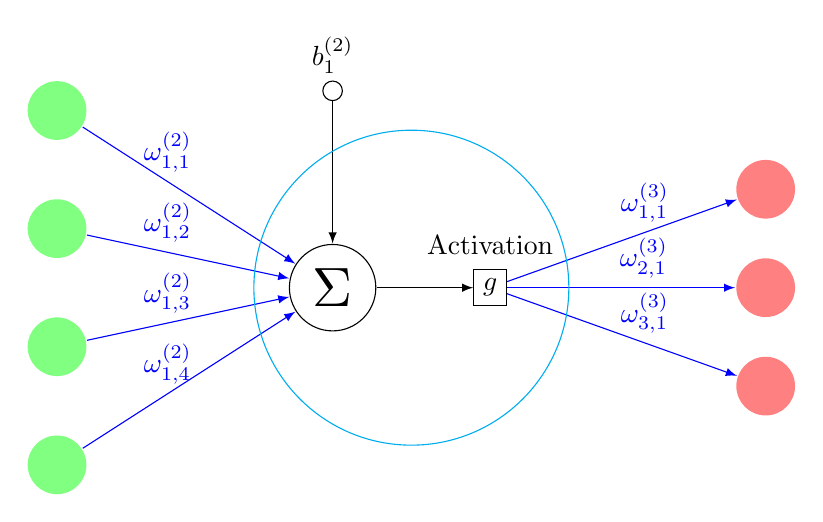
\begin{tikzpicture}[>=latex]
\path
(0,0)     node[circle,draw,scale=2,inner sep=2pt] (S) {$\Sigma$}
+(90:2.5) node[circle,draw,inner sep=2.5pt] (b) {}
          node[above=1mm] {$b_1^{(2)}$}
+(-3.5,2.25)  node[circle,scale=2.25,fill=green!50]  (x1) {} %{$T_{2m}$}
+(-3.5,0.75)  node[circle,scale=2.25,fill=green!50]  (x2) {} %{$q_v$}
+(-3.5,-0.75) node[circle,scale=2.25,fill=green!50]  (x3) {} %{$RH$}
+(-3.5,-2.25) node[circle,scale=2.25,fill=green!50]  (x4) {} %{$p_s$}
(2,0)    node[draw] (g) {$g$} node[above=3mm]{Activation}

+(3.5,1.25)  node[circle,scale=2.25,fill=red!50]  (y1) {}
+(3.5,0)  node[circle,scale=2.25,fill=red!50]  (y3) {}
+(3.5,-1.25) node[circle,scale=2.25,fill=red!50]  (y2) {};

\draw[->, black] (S)--(g);
\draw[->, black] (b)--(S);
\draw[->, blue] (g)--(y1) node[pos=.6,above, blue]{$\omega_{1,1}^{(3)}$};
\draw[->, blue] (g)--(y2) node[pos=.6,above, blue]{$\omega_{3,1}^{(3)}$};
\draw[->, blue] (g)--(y3) node[pos=.6,above, blue]{$\omega_{2,1}^{(3)}$};

\draw[->, blue] (x1)--(S) node[pos=.4,above, blue]{$\omega_{1,1}^{(2)}$};
\draw[->, blue] (x2)--(S) node[pos=.4,above, blue]{$\omega_{1,2}^{(2)}$};
\draw[->, blue] (x3)--(S) node[pos=.4,above, blue]{$\omega_{1,3}^{(2)}$};
\draw[->, blue] (x4)--(S) node[pos=.4,above, blue]{$\omega_{1,4}^{(2)}$};
\draw[cyan] (1,0) circle(2);
\end{tikzpicture}

\caption{Computational graph showing the components participating in the activation of a neuron in the hidden layer. This example shows a 2-layer neural network with four input nodes and three output nodes. The number of nodes in the hidden layer doesn't affect the activation, since they are not connected. The sum of the weighted input and bias is passed to the activation function,
inside the hidden layers. Producing the activation of the neuron. This is again passed to the output neurons. Modified skecth based on \href{https://tex.stackexchange.com/questions/505741/architecture-neural-network-with-weights}{https://tex.stackexchange.com/questions/505741/architecture-neural-network-with-weights}. }
\label{fig:activation_one_node}
\end{figure}
\begin{figure}
    \centering
    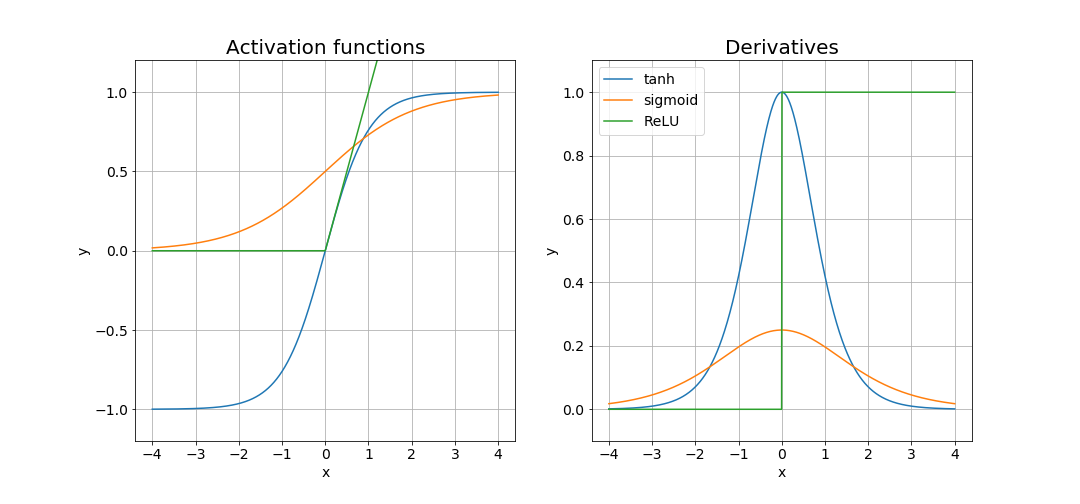
\includegraphics[scale = 0.4]{Chapter3_Method/figs/activation_functions_and_derivatives.png}
    \caption{Activation functions and their derivatives.}
    \label{fig:activation_function_example}
\end{figure}

Figure \ref{fig:activation_one_node} shows the computation which takes place in a node in the hidden layer, focusing on a circle in the middle column in Figure \ref{fig:one_layer_mlp}. The sum of the weighted inputs and bias are sent trough the activation function, $g$, producing the activation. This function, $g$, is a hyperparameter, set before the training starts. Popular choices are rectified linear unit (ReLU), sigmoid function  ($\sigma$) or hyperbolic tangent (tanh), their graphs are shown in Figure \ref{fig:activation_function_example} and their mathematical expressions in Equations \eqref{eq:ReLU}, \eqref{eq:sigmoid} and \eqref{eq:tanh} respectively.
\begin{equation} \label{eq:ReLU}
   ReLU\left(x\right) = 
     \begin{cases}
       \text{x,} &\quad\text{if x} \ge 0\\
       \text{0,} &\quad\text{else}
     \end{cases}
\end{equation}
\begin{equation} \label{eq:sigmoid}
   \sigma \left( x \right) = \frac{1}{1 + e^{-x}}
\end{equation}
\begin{equation} \label{eq:tanh}
   tanh\left( x \right) = \frac{e^x - e^{-x}}{e^x + e^{-x}} = \frac{e^{2x} - 1}{e^{2x} + 1}
\end{equation}
%Figure \ref{fig:activation_one_node} shows the computation which takes place in a node in the hidden layer, a dot the middle column in Figure \ref{fig:one_layer_mlp}. The sum of the weighted input and bias are sent trough the activation function, $g$, producing the activation. The activation function is a hyperparameter, set before the training starts. Popular choices are rectified linear unit (ReLU), sigmoid or tanh-function. These are shown in Figure \ref{fig:activation_function_example}.

Equation \eqref{eq:activation_hidden_pass} describes the activation of a node in a arbitrary layer, L. $b_L$ denotes the bias, $w_L$ is the weights matrix. and $n_L$ is the number of  nodes. $g_L$ denotes activation function in a arbitrary layer.
%For regression problem, $g_o$ is linear like.
\begin{equation} \label{eq:activation_hidden_pass}
    \textbf{a}_L = g_L\left(\sum_{i=1}^{n_L} \textbf{W}_{L, i} \textbf{x}_i + b_L\right)
\end{equation}
%\begin{equation} \label{eq:output_pass}
%    \textbf{a}_{L+1} = g_o(\sum_{i=1}^n \textbf{W}_{L+1, i} \textbf{a}_{L+1} + b_{L+1})
%\end{equation}
% \textbf{Thought to self, Notation is trick when the next layer is the output. Since the activation-function usually is different in hidden layers and output layers. }
% Recursively moving things to next layer.
Repeating the procedure for the next layer, $L+1$, the activation, $a_L$ from the previous layer is weighted and passed trough the activation function, $g_{L+1}$, generating the activation, $a_{L+1}$. In a forward pass, this is repeated for all layers, until the output layer is reached. Adapting Equation \eqref{eq:activation_hidden_pass} to the example in Figure \ref{eq:activation_hidden_pass} can be done by inserting $L=1$ and $n_L=4$.

The choice of activation function, $g$, in the output layer is task specific. Regression problems use linear activation. Classification problem need functions able to discriminate between the number of classes.

Backpropagation is the fundamental mechanism used in ``teaching'' neural networks. First appreciated in its full importance in \citeyear{RumelhartBackProp} when it was published by \citeauthor{RumelhartBackProp}. The trick is to use the performance metric as a feedback signal to adjust the weights in the direction of the lowest loss score for the current example. A training instance is passed trough the network producing a output (red node). The networks output error is computed as difference between the computed output and the corresponding targets. For each consecutive layer, moving in reverse from the output to the input, the contribution from every connection between adjacent layers is computed.
For a more mathematical description of the backpropagation algorithm see \cite{nielsen_back_prop}.

\subsection{Convolutional neural networks} \label{sec:convolutional neural network}
%\textit{According to the philosophy underlying deep learning approach, if we have a reasonable end-to-end model and a sufficient data for training it, we are close to solving the problem}. (Shi et. al., 2015). 
Computer vision is a field of artificial intelligence concerned with interpreting the visual world. One popular structure for visual tasks is the convolutional neural network. %Its said to resemble the visual cortex, the centre in the brain which processes the visual information. 
\begin{figure}
    \centering
    
    \begin{tikzpicture}[scale=1.5,every node/.style={minimum size=1cm}, on grid]
    % slanting: production of a set of n 'laminae' to be piled up.
    % N=number of grids.
    
            
        \begin{scope}[yshift=-200, xshift = -200, 
                      every node/.append style={yslant=0.,xslant=0},
                      yslant=0,xslant=0]
            \draw[black, very thick, fill = gray, opacity = 0.2] (0,0) rectangle (2.8, 3.6);
            \draw[step = 4mm, very thick, black] (0,0) grid (2.8, 3.6);
            \coordinate (s9) at (0.2, 3.4);
            \node at (s9) [circle, scale=1.5] {$P$};
            
        \end{scope} 
        
    
        % RED LAYER 
        \begin{scope}[yshift=-200,every node/.append style={
            yslant=0.5,xslant=-1.3},yslant=0.5,xslant=-1.3 ]
            \draw[black, very thick, fill = red, opacity = 0.2] (0,0) rectangle (2.1, 2.7); % marking borders 
            \draw[black, very thick] (0,0) rectangle (2.1, 2.7); % marking borders
            
            \coordinate (s9) at (0, 0);
            \coordinate (s10) at (0, 2.7);
            \coordinate (s11) at (2.1, 0);
            \coordinate (s12) at (2.1, 2.7);

            \coordinate (t1) at (0, 0.3);
            %\node at (t1) [circle, fill = blue, scale=.5] {$P$};
            
            \coordinate (t2) at (0, 0.6);
            %\node at (t2) [circle, fill = blue, scale=.5] {$P$};
            
            \coordinate (t3) at (0, 0.9);
            %\node at (t3) [circle, fill = blue, scale=.5] {$P$};
            
            \coordinate (t4) at (0, 1.2);
            %\node at (t4) [circle, fill = blue, scale=.5] {$P$};
            
            \coordinate (t5) at (0, 1.5);
            %\node at (t5) [circle, fill = blue, scale=.5] {$P$};
            
            \coordinate (t6) at (0, 1.8);
            %\node at (t6) [circle, fill = blue, scale=.5] {$P$};
            
            \coordinate (t7) at (0, 2.1);
            %\node at (t7) [circle, fill = blue, scale=.5] {$P$};
            
            \coordinate (t8) at (0, 2.4);
            %\node at (t8) [circle, fill = blue, scale=.5] {$P$};
            
            \coordinate (t9) at (0.3, 0);
            %\node at (t9) [circle, fill = blue, scale=.5] {$P$};
            
            \coordinate (t10) at (0.6, 0);
            %\node at (t10) [circle, fill = blue, scale=.5] {$P$};
            
            \coordinate (t11) at (0.9, 0);
            %\node at (t11) [circle, fill = blue, scale=.5] {$P$};
            
            \coordinate (t12) at (1.2, 0);
            %\node at (t12) [circle, fill = blue, scale=.5] {$P$};
            
            \coordinate (t13) at (1.5, 0);
            %\node at (t13) [circle, fill = blue, scale=.5] {$P$};
            
            \coordinate (t14) at (1.8, 0);
            %\node at (t14) [circle, fill = blue, scale=.5] {$P$};

            
        \end{scope} 
        
        
        \begin{scope}[
            yshift=-195,every node/.append style={
            yslant=0.5,xslant=-1.3},yslant=0.5,xslant=-1.3
                      ]
            \draw[black, very thick, fill = green, opacity = 0.2] (0,0) rectangle (2.1, 2.7); % marking borders 
            \coordinate (h_input) at (2.1, 0);
            \coordinate (h_bl) at (0, 2.7);
            %\node at (h_bl) [fill=blue, circle, scale=0.5] {$s$};
        \end{scope} 
        
        % BLUE LAYER 
        \begin{scope}[yshift=-190,every node/.append style={
                yslant=0.5,xslant=-1.3},yslant=0.5,xslant=-1.3]
                \draw[black, very thick, fill = blue, opacity = 0.2] (0,0) rectangle (2.1, 2.7); % marking borders 
                \draw[black, very thick] (0,0) rectangle (2.1, 2.7); % marking borders 
                %\draw[black, very thick] (0,0) rectangle (2.1, 2.7); % marking borders 
                \draw[step=3mm, very thick, black] (0, 0) grid (2.1, 2.7);
                
                \coordinate (s1) at (0, 0);
                \coordinate (s2) at (0, 2.7);
                \coordinate (s3) at (2.1, 0);
                \coordinate (s4) at (2.1, 2.7);
    
                \draw[black,very thick]   (s9) -- (s1);
                \draw[black,very thick]   (s10) -- (s2);
                \draw[black,very thick]   (s11) -- (s3);
                \draw[black,very thick]   (s12) -- (s4);
                
                \coordinate (s9) at (0.15, 2.55);
                \node at (s9) [circle, scale=1.5] {$P$};
                
            \coordinate (h1) at (0, 0.3);
            %\node at (t1) [circle, fill = blue, scale=.5] {$P$};
            
            \coordinate (h2) at (0, 0.6);
            %\node at (t2) [circle, fill = blue, scale=.5] {$P$};
            
            \coordinate (h3) at (0, 0.9);
            %\node at (t3) [circle, fill = blue, scale=.5] {$P$};
            
            \coordinate (h4) at (0, 1.2);
            %\node at (t4) [circle, fill = blue, scale=.5] {$P$};
            
            \coordinate (h5) at (0, 1.5);
            %\node at (t5) [circle, fill = blue, scale=.5] {$P$};
            
            \coordinate (h6) at (0, 1.8);
            %\node at (t6) [circle, fill = blue, scale=.5] {$P$};
            
            \coordinate (h7) at (0, 2.1);
            %\node at (t7) [circle, fill = blue, scale=.5] {$P$};
            
            \coordinate (h8) at (0, 2.4);
            %\node at (t8) [circle, fill = blue, scale=.5] {$P$};
            
            \coordinate (h9) at (0.3, 0);
            %\node at (t9) [circle, fill = blue, scale=.5] {$P$};
            
            \coordinate (h10) at (0.6, 0);
            %\node at (t10) [circle, fill = blue, scale=.5] {$P$};
            
            \coordinate (h11) at (0.9, 0);
            %\node at (t11) [circle, fill = blue, scale=.5] {$P$};
            
            \coordinate (h12) at (1.2, 0);
            %\node at (t12) [circle, fill = blue, scale=.5] {$P$};
            
            \coordinate (h13) at (1.5, 0);
            %\node at (t13) [circle, fill = blue, scale=.5] {$P$};
            
            \coordinate (h14) at (1.8, 0);
            %\node at (t14) [circle, fill = blue, scale=.5] {$P$};
                
        \end{scope}
        
        \draw[black,very thick]   (t1) -- (h1);
        \draw[black,very thick]   (t2) -- (h2);
        \draw[black,very thick]   (t3) -- (h3);
        \draw[black,very thick]   (t4) -- (h4);
        \draw[black,very thick]   (t5) -- (h5);
        \draw[black,very thick]   (t6) -- (h6);
        \draw[black,very thick]   (t7) -- (h7);
        \draw[black,very thick]   (t8) -- (h8);
        \draw[black,very thick]   (t9) -- (h9);
        \draw[black,very thick]   (t10) -- (h10);
        \draw[black,very thick]   (t11) -- (h11);
        \draw[black,very thick]   (t12) -- (h12);
        \draw[black,very thick]   (t13) -- (h13);
        \draw[black,very thick]   (t14) -- (h14);
    
    
    \end{tikzpicture}    
    
    \caption{Transforming t 2D image to a 3D tensor. Decoding a image into RGB (red green blue) channels. Inspired by Figure 1 in \cite{precip_nowcasting}.}
    \label{fig:2D_image}
\end{figure}







Computers see images as a grid of numbers, often decoded in red, green and blue (RGB) channels. Figure \ref{fig:2D_image} shows the transformation of a two-dimensional image to a 3-dimensional tensor. The ``P'' shows the connection between one pixel (``picture element'') and a volume. Each of the grid cells (pixels) contains the signal from the colour decoded into values ranging from 0 to 255. The machine needs to learn how to extract the necessary information about these pixels to perform a task. More layers increase the model's ability to extract these complex structures, resulting in improved model performance. 
% kilde https://tex.stackexchange.com/questions/522118/visualizing-matrix-convolution 
\begin{figure}[h] % h means place here if possible
    \centering
    \begin{tikzpicture}[mmat/.style={matrix of math nodes,column sep=-\pgflinewidth/2,
   row sep=-\pgflinewidth/2,cells={nodes={draw,inner sep=2pt,thin}},draw=#1,thick, inner sep=0pt},
   mmat/.default=green,
   node distance=0.3em]
   
 \matrix[mmat](mat1){
         0 & 1 & 1 & |[draw=green,thick,fill=green!20,alias=1]| 1 & |[draw=green,thick,fill=green!20,alias=0]| 0 & |[draw=green,thick,fill=green!20,alias=]| 0 & 0 \\ 
         0 & 0 & 1 & |[draw=green,thick,fill=green!20,alias=1]|1 & |[draw=green,thick,fill=green!20,alias=1]|1 &|[draw=green,thick,fill=green!20,alias=0]| 0 & 0 \\ 
         0 & 0 & 0 & |[draw=green,thick,fill=green!20,alias=1]|1 &|[draw=green,thick,fill=green!20,alias=1]| 1 & |[draw=green,thick,fill=green!20,alias=1]|1 & 0 \\ 
         0 & 0 & 0 & 1 & 1 & 0 & 0 \\ 
         0 & 0 & 1 & 1 & 0 & 0 & 0 \\ 
         0 & 1 & 1 & 0 & 0 & 0 & 0 \\ 
         0 & 1 & 0 & 0 & 0 & 0 & 0 \\ 
         };
 \node[fit=(mat1-1-4)(mat1-3-6),inner sep=0pt, draw, green, thick, fill = green, opacity = 0.2](f1){};        
 
 \node[right=of mat1] (mul) {$*$};      
 \matrix[mmat=blue,fill=blue!30,right=of mul](mat2){    
     1 & 0 & 1 \\ 
     0 & 1 & 0 \\ 
     1 & 0 & 1 \\ };
 \node[right=of mat2] (eq) {$=$};       
 \matrix[mmat,right=of eq, draw = red](mat3){    
     1 & 4 & 3 & |[draw=red,thick,fill=red!20,alias=4]|4 & 1 \\ 
     1 & 2 & 4 & 3 & 3 \\ 
     1 & 2 & 3 & 4 & 1 \\ 
     1 & 3 & 3 & 1 & 1 \\ 
     3 & 3 & 1 & 1 & 0 \\ 
 };
 \foreach \Anchor in {south west,north west,south east,north east}
 {\draw[blue,densely dotted] (f1.\Anchor) -- (mat2.\Anchor); 
 \draw[red,densely dotted] (4.\Anchor) -- (mat2.\Anchor);}
 \begin{scope}[on background layer]
  \fill[red!20] (f1.north west) rectangle (f1.south east);
 \end{scope}
\end{tikzpicture}
    \caption{Diagram showing a convolutional operation. Modified sketch based on \cite{convolution_operation}.}
    \label{fig:convolution}
\end{figure}
Figure \ref{fig:convolution} shows the mathematical operation convolution as the sum over element-wise multiplication of the filter and input. The filter is blue, this is placed over the filled green section, producing the red output pixel. The entire red grid is called a feature map (output map). The green grid is the input, overlaid with blue indicating the pixels contributing to the activation, of the red pixel. In Figure \ref{fig:convolution} this would be the value 4. \textit{Receptive field} is known as the pixels contributing to the activation in a pixel (i.e. the value) (\cite{Luo2016UnderstandingNetworks}). For instance the receptive field of the shaded red pixel is the shaded green submatrix.
%Figure \ref{fig:convolution} shows the mathematical operation convolution as the sum over element-wise multiplication of the filter and input. The filter is blue, this is placed over the filled green section, producing the red output pixel. The entire red grid is called a feature map (output map). The green grid is the input, overlaid with blue illustrated the pixels contributing to the activation, red pixel. In Figure \ref{fig:convolution} this would be the value 4. \textit{Receptive field} is known as the pixels contributing to the activation in a pixel (i.e. the value). For instance the receptive field of the shaded red pixel is the shaded green submatrix.


\begin{figure}
    \centering
    
    \begin{tikzpicture}[scale=2,every node/.style={minimum size=1cm},on grid]
    % slanting: production of a set of n 'laminae' to be piled up.
    % N=number of grids.
    \begin{scope}[
            yshift=-100, xshift= 0, every node/.append style={
            yslant=0.5, xslant=-1.3}, yslant=0.5, xslant=-1.3
            ]
        % opacity to prevent graphical interference
        \draw[red, very thick, fill = white]  (0, 0) rectangle (1.5, 2.1);
        \draw[step=3mm, thin, red] (0, 0) grid (1.5, 2.1);   % defining grids
        \draw[red, very thick] (0, 0) rectangle (1.5, 2.1); % marking borders    
        
        % pixel closest to output layes
        \coordinate (bl) at (0.16, 1.92);
        \node at (bl) [fill=red!80, square, scale=0.65] {};
        
        %last pixel
        \coordinate (pi) at (0.5, 1.92);
        \node at (pi) [fill=red!60, square, scale=0.65] {};
        
        % rightmost pixel
        \coordinate (cy) at (0.16, 0.16);
        \node at (cy) [fill=red!40, square, scale=0.64] {};
        
        \coordinate (input_c) at (0, 2.1);
        %\node at (corner) [fill=yellow, square, scale=0.64] {s};        
        
        \end{scope}
    
        \begin{scope}[
            yshift=-160,every node/.append style={
            yslant=0.5,xslant=-1.3},yslant=0.5,xslant=-1.3
                      ]
            % Marking border
            \draw[blue, very thick, fill = gray!70] (0,0) rectangle (2.1, 2.7);
            \draw[green, very thick, fill = green!20] (0.33, 0.33) rectangle (1.8, 2.4);
            \draw[step=3mm, thin, gray] (0,0) grid   (2.1, 2.7);  % defining grid padding
            \draw[step=3mm, thick, green] (0.33, 0.33) rectangle (1.8, 2.4); % defining grids
            \draw[black, very thick] (0,0) rectangle (2.1, 2.7);% marking borders   
            % \draw[black,very thick, fill = blue!50] (0,0) rectangle (3,3);

            \coordinate (s1) at (0, 2.7);
            %\node at (s1) [fill=blue, circle, scale=0.5] {$s$};
            \coordinate (s2) at (0, 1.8);
            %\node at (s2) [fill=pink, circle, scale=0.5] {$s$};
            \coordinate (s3) at (0.9, 1.8);
            %\node at (s3) [fill=yellow, circle, scale=0.5] {$s$};
            \coordinate (s4) at (0.9, 2.7);
            %\node at (s4) [fill=blue, circle, scale=0.5] {$s$};
                      
            \draw[draw=blue, very thick, line join=round, dashed, fill = blue, opacity = 0.5] %  opacity=.2, 
                  (0,  2.7) -- 
                  (0,  1.8) --
                  (0.9,  1.8) --
                  (0.9,  2.7) -- cycle ;
                
            \draw[fill=white, draw=blue, opacity=.5, very thick, line join=round]
            (s4) -- (bl);
            
            \draw[fill=white, draw=blue, opacity=.5, very thick, line join=round]
            (s3) -- (bl);
 
            \draw[fill=white, draw=blue, opacity=.5, very thick, line join=round]
            (s2) -- (bl);
            
            \draw[fill=white, draw=blue, opacity=.5, very thick, line join=round]
            (s1) -- (bl);
           
           %%%%%%%%%%%%%%%%%%%%%%%% PINK
            \coordinate (s5) at (0.333, 2.7);
            %\node at (s5) [fill=blue, circle, scale=0.5] {$s$};

            \coordinate (s6) at (0.333, 1.8);
            %\node at (s6) [fill=pink, circle, scale=0.5] {$s$};

            \coordinate (s7) at (1.2333, 1.8);
            %\node at (s7) [fill=yellow, circle, scale=0.5] {$s$};

            \coordinate (s8) at (1.2333, 2.7);
            %\node at (s8) [fill=blue, circle, scale=0.5] {$s$};
           
           
           
            \draw[draw=blue, very thick, line join=round, opacity=.2, fill = blue, opacity = 0.5] %  opacity=.2, 
                  (s5) -- (s6) -- (s7) -- (s8) -- cycle;

            \draw[fill=white, draw=blue, opacity=0.5, very thick, line join=round, dashed]
            (s5) -- (pi);
            
            \draw[fill=white, draw=blue, opacity=0.5, very thick, line join=round, dashed]
            (s6) -- (pi);
 
            \draw[fill=white, draw=blue, opacity=.5, very thick, line join=round, dashed]
            (s7) -- (pi);
            
            \draw[fill=white, draw=blue, opacity=.5, very thick, line join=round, dashed]
            (s8) -- (pi);
            
            %%%%%%%%%%%%%%%%%%%%%%%% blue
            \coordinate (s9) at (0, 0);
            %\node at (s5) [fill=blue, circle, scale=0.5] {$s$};

            \coordinate (input_layer) at (0.32, 1);
            %\node at (input_layer) [fill=blue, circle, scale=0.5] {$s$};

            \coordinate (s10) at (0, 0.9);
            %\node at (s6) [fill=pink, circle, scale=0.5] {$s$};

            \coordinate (s11) at (0.9, 0.9);
            %\node at (s7) [fill=yellow, circle, scale=0.5] {$s$};

            \coordinate (s12) at (0.9, 0);
            %\node at (s8) [fill=blue, circle, scale=0.5] {$s$};
           
            % Adding coordinates for padding
            \coordinate (p1) at (2.1, 0);
            \coordinate (p2) at (1.8, 0);

            \draw[draw=blue!60, very thick, line join=round, dashed, opacity=.6, fill = blue!60] %  opacity=.2, 
                  (s9) -- (s10) -- (s11) -- (s12) -- cycle;

            \draw[fill=white, draw=blue!60, opacity=.6, very thick, line join=round]
            (s9) -- (cy);
            
            \draw[fill=white, draw=blue!60, opacity=.6, very thick, line join=round]
            (s10) -- (cy);
 
            \draw[fill=white, draw=blue!60, opacity=.6, very thick, line join=round]
            (s11) -- (cy);
            
            \draw[fill=white, draw=blue!60, opacity=.6, very thick, line join=round]
            (s12) -- (cy);
            
        \end{scope} %end of drawing grids
    
       \draw[-latex,thick](-1, -6)node[left, scale=1.3]{Input layer}
             to[out=0, in=90] (input_layer);  	
            
        \draw[-latex,thick](2.7, -4.25)node[above, scale=1.3]{Zero padding}
             to[out=0, in=90] (p1);  
        \draw[-latex,thick](2.7, -4.25)node[above, scale=1.3]{}
             to[out=0, in=90] (p2);      
             
       \draw[-latex,thick](-3, -2.5)node[left, scale=1.3]{Output layer}
             to[out=0,in=90] (input_c);  	
        
        \draw[-latex,thick](-4, -5)node[left, scale=1.3]{$f_w = 3$}
               to[out=0,in=90] (s1);  	
        \draw[-latex,thick](-4, -5)node[left]{}
              to[out=0,in=90] (s2);  	
            
        \draw[-latex,thick](-3.7, -4.4)node[left, scale=1.3]{$f_h = 3$}
               to[out=0,in=90] (s1);  	
        \draw[-latex,thick](-3.7, -4.4)node[left]{}
              to[out=0,in=90] (s4);  
    \end{tikzpicture}
    \caption{The illustration shows the connections between input and output layer. This example uses a $3\times 3$-filter (blue), zero-padding (gray) resulting in equal dimensions for input (green) and output (red). The different colors illustrate the connections between input and output pixels. The input pixels contributing to the output, is called the receptive field. The zero padding is added to keep the input shape. Inspired by Figure (13-3) in \cite{OReiley_book}. 
    }
    \label{fig:convolution_padding}
\end{figure}

Convolving a filter over the input image generates a feature map, a 2-dimensional activation. If it happens to be the last layer, it is common to refer to the results as the output instead, although this is merely a difference in terminology. Figure \ref{fig:convolution_padding} shows a 2D-convolution with filter of size $3\times 3$. Filters are often square (not a strict requirement), and the height $f_h$ and width $f_w$ are odd numbers. The origin is the position of the kernel which is above the current output pixels. The connections between the layers are intended to illustrate the part contributing to the pixel, as well as highlighting the receptive field. In order to include the outermost pixels, the input area is padded with zeros around the edges (grey boarder). 
%Convolving a filter over the input image generates a feature map. If it happens to be the last layer, it is common to refer to the results as the output instead, even though there is no difference. Figure \ref{fig:convolution_padding} shows a 2D-convolution with filter of size $3\times 3$. Filters are often square (not a strict requirement) and the height, $f_h$ and $f_w$ are odd numbers (not a strict requirement either). The origin is the position of the kernel which is above the current output pixels. The connections between the layers are intended to illustrate the part contributing to the pixel, as well as highlighting the receptive field. In order to include the outermost pixels, the input area is padded with zeros around the edges (shown as gray in the figure). 
\begin{figure}
    \centering
   \begin{tikzpicture}[scale=1.7,every node/.style={minimum size=1cm},on grid]
    % slanting: production of a set of n 'laminae' to be piled up.
    % N=number of grids.

        \begin{scope}[
            yshift=-200,every node/.append style={
            yslant=0.5,xslant=-1.3},yslant=0.5,xslant=-1.3
                      ]
            \draw[black, very thick, fill = red, opacity = 0.2] (0,0) rectangle (2.1, 2.7); % marking borders 
            \draw[black, very thick] (0,0) rectangle (2.1, 2.7); % marking borders 

            \coordinate (s9) at (0, 0);
            %\node at (s9) [fill=blue, circle, scale=0.5] {$s$};
            \coordinate (s10) at (0, 2.7);
            %\node at (s10) [fill=pink, circle, scale=0.5] {$s$};
            \coordinate (s11) at (2.1, 0);
            %\node at (s11) [fill=yellow, circle, scale=0.5] {$s$};
            \coordinate (s12) at (2.1, 2.7);
            %\node at (s12) [fill=cyan, circle, scale=0.5] {$s$};
            \coordinate (h_re) at (0, 2.7);
            %\node at (h_re) [fill=red, circle, scale=0.5] {$s$};
                                   
            % begynner i punkt (x, y) rectangle (x dim, y dim)
            \draw[black, very thick, dashed] (0.5, 0.95) rectangle (1.25, 1.25);
            \coordinate (o1) at (0.5, 0.95);
            %\node at (p1) [draw=black, very thick, circle, scale=0.3] {};
            \coordinate (o2) at (0.5, 0.95+1.25/2);
            %\node at (p2) [draw=black, very thick, circle, scale=0.3] {};
            \coordinate (o3) at (0.5+1.25/2+0.1, 0.95);
            %\node at (p3) [draw=black, very thick, circle, scale=0.3] {};
            \coordinate (o4) at (0.5+1.25/2+0.1, 0.95+1.25/2);
            %\node at (p4) [draw=black, very thick, circle, scale=0.3] {};

           
            % begynner i punkt (x, y) rectangle (x dim, y dim)
            \draw[black, very thick, dashed] (0.5, 0.95) rectangle (1.25, 1.6);
            \coordinate (z1) at (0.5, 0.95);
            %\node at (q1) [draw=black, very thick, circle, scale=0.3] {};
            \coordinate (z2) at (0.5, 0.95+1.25/2);
            %\node at (q2) [draw=black, very thick, circle, scale=0.3] {};
            \coordinate (z3) at (0.5+1.25/2+0.1, 0.95);
            %\node at (q3) [draw=black, very thick, circle, scale=0.3] {};
            \coordinate (z4) at (0.5+1.25/2+0.1, 0.95+1.25/2);
            %\node at (q4) [draw=black, very thick, circle, scale=0.3] {};


            %\draw[black, very thick, dashed] (0.8, 0.45) rectangle (1.25, 1.6);
            \coordinate (x1) at (0.8, 0.45);
            %\node at (u1) [draw=black, very thick, circle, scale=0.3] {};
            \coordinate (x2) at (0.8, 0.45+1.25/2);
            %\node at (u2) [draw=black, very thick, circle, scale=0.3] {};
            \coordinate (x3) at (0.8+1.25/2+0.1, 0.45);
            %\node at (u3) [draw=black, very thick, circle, scale=0.3] {};
            \coordinate (x4) at (0.8+1.25/2+0.1, 0.45+1.25/2);
            %\node at (u4) [draw=black, very thick, circle, scale=0.3] {};
            \draw[black,very thick, dashed]   (x1) -- (x3) -- (x4) -- (x2) --(x1);
        \end{scope} 

        \begin{scope}[
            yshift=-195,every node/.append style={
            yslant=0.5,xslant=-1.3},yslant=0.5,xslant=-1.3
                      ]
            \draw[black, very thick, fill = green, opacity = 0.2] (0,0) rectangle (2.1, 2.7); % marking borders 
            \coordinate (h_input) at (2.1, 0);
            \coordinate (h_bl) at (0, 2.7);
            %\node at (h_bl) [fill=blue, circle, scale=0.5] {$s$};
        \end{scope} 
           
           \draw[thick](3, -5.7)node[scale=1.3]{Input Layer};
           \draw[thick](3.5, -3.2)node[scale=1.3]{Convolutional layer 1};
           \draw[thick](3.5, -0.7)node[scale=1.3]{Convolutional layer 2};
           \draw[thick](-4.6, -0.2)node[scale=1.3]{Feature};
           \draw[thick](-4.6, -1.1)node[scale=1.3]{$\vdots$};
           \draw[thick](-4.6, -3.6)node[scale=1.3]{$\vdots$};
           \draw[thick](-4.4, -5.5)node[scale=1.3]{Channels};
           
        \begin{scope}[
            yshift=-190,every node/.append style={
            yslant=0.5,xslant=-1.3},yslant=0.5,xslant=-1.3
                      ]
            \draw[black, very thick, fill = blue, opacity = 0.2] (0,0) rectangle (2.1, 2.7); % marking borders 
            \draw[black, very thick] (0,0) rectangle (2.1, 2.7); % marking borders 

            \coordinate (s1) at (0, 0);
            \coordinate (s2) at (0, 2.7);
            \coordinate (s3) at (2.1, 0);
            \coordinate (s4) at (2.1, 2.7);

            \draw[black,very thick]   (s9) -- (s1);
            \draw[black,very thick]   (s10) -- (s2);
            \draw[black,very thick]   (s11) -- (s3);
            \draw[black,very thick]   (s12) -- (s4);
                        
            \coordinate (h_gr) at (0, 2.7);

            % begynner i punkt (x, y) rectangle (x dim, y dim)
            \draw[black, very thick, dashed] (0.5, 0.95) rectangle (1.25, 1.6);
            \coordinate (q1) at (0.5, 0.95);
            %\node at (q1) [draw=black, very thick, circle, scale=0.3] {};
            \coordinate (q2) at (0.5, 0.95+1.25/2);
            %\node at (q2) [draw=black, very thick, circle, scale=0.3] {};
            \coordinate (q3) at (0.5+1.25/2+0.1, 0.95);
            %\node at (q3) [draw=black, very thick, circle, scale=0.3] {};
            \coordinate (q4) at (0.5+1.25/2+0.1, 0.95+1.25/2);
            %\node at (q4) [draw=black, very thick, circle, scale=0.3] {};

            %\draw[black, very thick, dashed] (0.8, 0.45) rectangle (1.25, 1.6);
            \coordinate (u1) at (0.8, 0.45);
            %\node at (u1) [draw=black, very thick, circle, scale=0.3] {};
            \coordinate (u2) at (0.8, 0.45+1.25/2);
            %\node at (u2) [draw=black, very thick, circle, scale=0.3] {};
            \coordinate (u3) at (0.8+1.25/2+0.1, 0.45);
            %\node at (u3) [draw=black, very thick, circle, scale=0.3] {};
            \coordinate (u4) at (0.8+1.25/2+0.1, 0.45+1.25/2);
            %\node at (u4) [draw=black, very thick, circle, scale=0.3] {};

            \draw[black,very thick, dashed]   (u1) -- (u3) -- (u4) -- (u2) --(u1);

            % Draws horizontal lines completing the litle cube.
            \draw[black,very thick, dashed]   (q1) -- (z1);
            \draw[black,very thick, dashed]   (q2) -- (z2);
            \draw[black,very thick, dashed]   (q3) -- (z3);
            \draw[black,very thick, dashed]   (q4) -- (z4);
            
            % Draws horizontal lines completing the litle cube.
            \draw[black,very thick, dashed]   (u1) -- (x1);
            \draw[black,very thick, dashed]   (u2) -- (x2);
            \draw[black,very thick, dashed]   (u3) -- (x3);
            \draw[black,very thick, dashed]   (u4) -- (x4);
            
        \end{scope} 

        \draw[black, thick, ->](-4.2, -5.95)node[left, scale=1.3]{green} to (h_bl);
        \draw[thick, ->](-4.2, -6.15)node[left, scale=1.3]{red} to (h_re);
        \draw[thick, ->](-4.2, -5.75)node[left, scale=1.3]{blue} to (h_gr);
        %%%%%%%%%%%%%%%%%%%%%%%% END OF INPUT LAYER 


        \begin{scope}[
            yshift=-140, every node/.append style={
            yslant=0.5,xslant=-1.3},yslant=0.5,xslant=-1.3]
            \draw[black, very thick, fill = gray, opacity = 0.2] (0,0) rectangle (2.1, 2.7); % marking borders 
            % Draws the boundary boxes
            \draw[black, very thick] (0,0) rectangle (2.1, 2.7);
            \coordinate (e5) at (0, 0);
            \coordinate (e6) at (0, 2.7);
            \coordinate (e7) at (2.1, 0);
            \coordinate (e8) at (2.1, 2.7);


            % draw left cylinder
            \coordinate (f) at (0.7, 1.1);
            \node at (f) [draw=black, very thick, circle, scale=0.3] {};
            \coordinate (f1) at (0.7, 1.15);
            %\node at (f1) [draw=red, very thick, circle, scale=0.3] {};
            \coordinate (f2) at (0.7, 1.05);
            %\node at (f2) [draw=red, very thick, circle, scale=0.3] {};
            
            % Draws the other
            \coordinate (g) at (1.1, 0.85);
            \node at (g) [draw=black, very thick, circle, scale=0.3] {};
            \coordinate (g1) at (1.1, 0.95);
            \coordinate (g2) at (1.1, 0.8);
            
            % Drawing the smaller lower 
            \draw[black, very thick, dashed] (0.5, 0.65) rectangle (1.25, 1.25);
            \coordinate (o1) at (0.5, 0.65);
            %\node at (o1) [draw=black, very thick, circle, scale=0.3] {};
            \coordinate (o2) at (0.5, 0.65+1.25/2);
            %\node at (o2) [draw=black, very thick, circle, scale=0.3] {};
            \coordinate (o3) at (0.5+1.25/2+0.1, 0.65);
            %\node at (o3) [draw=black, very thick, circle, scale=0.3] {};
            \coordinate (o4) at (0.5+1.25/2+0.1, 0.65+1.25/2);
            %\node at (o4) [draw=black, very thick, circle, scale=0.3] {};
  
        \end{scope} 
        
        \begin{scope}[
            yshift=-135,every node/.append style={
            yslant=0.5,xslant=-1.3},yslant=0.5,xslant=-1.3
                      ]
            \draw[black, very thick, fill = gray, opacity = 0.2] (0,0) rectangle (2.1, 2.7); % marking borders 
        \end{scope} 
    
        \begin{scope}[
            yshift=-130,every node/.append style={
            yslant=0.5,xslant=-1.3},yslant=0.5,xslant=-1.3
                      ]
            \draw[black, very thick, fill = gray, opacity = 0.2] (0,0) rectangle (2.1, 2.7); % marking borders 
        \end{scope} 
    

        \begin{scope}[
            yshift=-125, every node/.append style={
            yslant=0.5,xslant=-1.3},yslant=0.5,xslant=-1.3
                      ]
            \draw[black, very thick, fill = gray, opacity = 0.2] (0,0) rectangle (2.1, 2.7); % marking borders 
            \coordinate (h) at (2.1, 0);
            %\node at (h) [fill=blue, circle, scale=0.5] {$s$};
        \end{scope} 
        
        \begin{scope}[
            yshift=-120,every node/.append style={
            yslant=0.5,xslant=-1.3},yslant=0.5,xslant=-1.3
                      ]
            \draw[black, very thick, fill = gray, opacity = 0.2] (0,0) rectangle (2.1, 2.7); % marking borders 
        \end{scope} 
    
        \begin{scope}[
            yshift=-115,every node/.append style={
            yslant=0.5,xslant=-1.3},yslant=0.5,xslant=-1.3
                      ]
            \draw[black, very thick, fill = gray, opacity = 0.2] (0,0) rectangle (2.1, 2.7); % marking borders 
            
            % Connections to maps
            \coordinate (sec_map_L2) at (0, 2.7);
            %\node at (sec_map_L2) [fill=blue, circle, scale=0.5] {$s$};
            
        \end{scope} 
    
        \begin{scope}[
            yshift=-110,every node/.append style={
            yslant=0.5,xslant=-1.3},yslant=0.5,xslant=-1.3
                      ]
            \draw[black, very thick, fill = gray, opacity = 0.2] (0,0) rectangle (2.1, 2.7); % marking borders 
                    
            % Connections to maps
            \coordinate (sec_map_L1) at (0, 2.7);
            %\node at (sec_map_L1) [fill=blue, circle, scale=0.5] {$s$};
            
          \coordinate (e1) at (0, 0);
          \coordinate (e2) at (0, 2.7);
          \coordinate (e3) at (2.1, 0);
          \coordinate (e4) at (2.1, 2.7);

            \draw[black, very thick] (0,0) rectangle (2.1, 2.7); % draw boundaries
            % draws horizontal lines
            \draw[black,very thick]   (e5) -- (e1);
            \draw[black,very thick]   (e6) -- (e2);
            \draw[black,very thick]   (e7) -- (e3);
            \draw[black,very thick]   (e8) -- (e4);
            
            % begynner i punkt (x, y) rectangle (x dim, y dim)
            \draw[black, very thick, dashed] (0.5, 0.65) rectangle (1.25, 1.25);
            \coordinate (p1) at (0.5, 0.65);
            %\node at (p1) [draw=black, very thick, circle, scale=0.3] {};
            \coordinate (p2) at (0.5, 0.65+1.25/2);
            %\node at (p2) [draw=black, very thick, circle, scale=0.3] {};
            \coordinate (p3) at (0.5+1.25/2+0.1, 0.65);
            %\node at (p3) [draw=black, very thick, circle, scale=0.3] {};
            \coordinate (p4) at (0.5+1.25/2+0.1, 0.65+1.25/2);
            %\node at (p4) [draw=black, very thick, circle, scale=0.3] {};

            % Draws horizontal lines completing the litle cube.
            \draw[black,very thick, dashed]   (p1) -- (o1);
            \draw[black,very thick, dashed]   (p2) -- (o2);
            \draw[black,very thick, dashed]   (p3) -- (o3);
            \draw[black,very thick, dashed]   (p4) -- (o4);
            
            % draw one cylinder
            \coordinate (w) at (0.7, 1.1);
            \node at (w) [draw=black, very thick, circle, scale=0.3] {};
            \coordinate (w1) at (0.7, 1.15);
            %\node at (f1) [draw=red, very thick, circle, scale=0.3] {};
            \coordinate (w2) at (0.7, 1.05);
            %\node at (f2) [draw=red, very thick, circle, scale=0.3] {};
            
            % Draws the other
            \coordinate (r) at (1.1, 0.85);
            \node at (r) [draw=black, very thick, circle, scale=0.3] {};
            \coordinate (r1) at (1.1, 0.95);
            \coordinate (r2) at (1.1, 0.8);

            \draw[black, very thick, dashed]   (f1) -- (w1);
            \draw[black, very thick, dashed]   (f2) -- (w2);

            \draw[black, very thick, dashed]   (g1) -- (r1);
            \draw[black, very thick, dashed]   (g2) -- (r2);


            % Connnection between layers 
            \draw[black,very thick, dashed]   (q1) -- (f);
            \draw[black,very thick, dashed]   (q2) -- (f);
            \draw[black,very thick, dashed]   (q3) -- (f);
            \draw[black,very thick, dashed]   (q4) -- (f);
            
            % Connnection between layers 
            \draw[black,very thick, dashed]   (u1) -- (g);
            \draw[black,very thick, dashed]   (u2) -- (g);
            \draw[black,very thick, dashed]   (u3) -- (g);
            \draw[black,very thick, dashed]   (u4) -- (g);
            

        \end{scope} 
    
    
    
    
    
    %%%%%%%%%%%%%%%%%%%%%%%%%%%%% CONVOLUTIONAL LAYER 2
        
        \begin{scope}[
            yshift=-50,every node/.append style={
            yslant=0.5,xslant=-1.3},yslant=0.5,xslant=-1.3
                      ]
            \draw[black, very thick, fill = gray, opacity = 0.2] (0,0) rectangle (2.1, 2.7); % drawing layer 
            \coordinate (h) at (2.1, 0);
            %\node at (h) [fill=blue, circle, scale=0.5] {$s$};
            
        \end{scope} 

        \begin{scope}[
            yshift=-55,every node/.append style={
            yslant=0.5,xslant=-1.3},yslant=0.5,xslant=-1.3
                      ]
            \draw[black, very thick, fill = gray, opacity = 0.2] (0,0) rectangle (2.1, 2.7); % marking borders 
        \end{scope} 
        
        \begin{scope}[
            yshift=-60,every node/.append style={
            yslant=0.5,xslant=-1.3},yslant=0.5,xslant=-1.3
                      ]
                      
            % The outer box
            \draw[black, very thick, fill = gray, opacity = 0.2] (0,0) rectangle (2.1, 2.7); % marking borders 
            \coordinate (a5) at (0, 0);
            \coordinate (a6) at (0, 2.7);
            \coordinate (a7) at (2.1, 0);
            \coordinate (a8) at (2.1, 2.7);
            \draw[black, very thick] (0,0) rectangle (2.1, 2.7); % draw boundaries
                    
            % The inner box
            \coordinate (h) at (1.1, 1.2); % this should be connected to the next layer
            \node at (h) [draw=black, very thick, circle, scale=0.3] {};
            \coordinate (h1) at (1.1, 1.25);
            \coordinate (h2) at (1.1, 1.15);
            
        \end{scope} 
    
            \begin{scope}[
            yshift=-45,every node/.append style={
            yslant=0.5,xslant=-1.3},yslant=0.5,xslant=-1.3
                      ]
            \draw[black, very thick, fill = gray, opacity = 0.2] (0,0) rectangle (2.1, 2.7); % marking borders 
            
            \coordinate (sec_map) at (0, 2.7);
            %\node at (sec_map) [fill=blue, circle, scale=0.5] {$s$};
            
        \end{scope} 
        
        \begin{scope}[
            yshift=-40,every node/.append style={
            yslant=0.5,xslant=-1.3},yslant=0.5,xslant=-1.3
                      ]
            \draw[black, very thick, fill = gray, opacity = 0.2] (0,0) rectangle (2.1, 2.7); % marking borders 
            \coordinate (a1) at (0, 0);
            \coordinate (a2) at (0, 2.7);
            \coordinate (a3) at (2.1, 0);
            \coordinate (a4) at (2.1, 2.7);

            \draw[black, very thick] (0,0) rectangle (2.1, 2.7); % draw boundaries
            % draws horizontal lines
            \draw[black,very thick]   (a5) -- (a1);
            \draw[black,very thick]   (a6) -- (a2);
            \draw[black,very thick]   (a7) -- (a3);
            \draw[black,very thick]   (a8) -- (a4);
            
            % Draws the cylinder
            \coordinate (i) at (1.1, 1.2);
            \node at (i) [draw=black, very thick, circle, scale=0.3] {};
            \node[right of=i, node distance=0.5cm] (p) {P};
            
            \coordinate (i1) at (1.1, 1.25); % for lines
            \coordinate (i2) at (1.1, 1.15); % for lines
            
            % drawing lines
            \draw[black,very thick, dashed]   (i1) -- (h1);
            \draw[black,very thick, dashed]   (i2) -- (h2);

            % Draw the lines connecting the first and second layer.
            \draw[black,very thick, dashed]   (p1) -- (h);
            \draw[black,very thick, dashed]   (p2) -- (h);
            \draw[black,very thick, dashed]   (p3) -- (h);
            \draw[black,very thick, dashed]   (p4) -- (h);

            \coordinate (first_map) at (0, 2.7);
            %\node at (first_map) [fill=blue, circle, scale=0.5] {$s$};

        \end{scope} 
    
        \draw[thick, ->](-4.2, -0.5)node[left, scale=1.3]{Map 1} to (first_map);
        \draw[thick, ->](-4.2, -0.8)node[left, scale=1.3]{Map 2} to (sec_map);
     
        \draw[thick, ->](-4.2, -3)node[left, scale=1.3]{Map 1} to (sec_map_L1);
        \draw[thick, ->](-4.2, -3.3)node[left, scale=1.3]{Map 2} to (sec_map_L2);
    % signed distance
    \end{tikzpicture}    
    \caption[Receptive field of pixel in convolutional neural network trained on RGB-image.]{First two layers of a convolutional neural network trained on RGB-images. Each convolutional layer contains multiple filters, thus producing stack of feature maps. Each layer learn the representation of the previous layer. The trailing layer get this stack as input, producing activations based on all channels. For each layer it contains representations of the structures found in the previous layer. The filters are the weights trained to find useful structures. In each convolutional layer multiple of these filters are passed over the image. The dashed volumes illustrate the receptive fields of a pixel, ``P''. The receptive field of a node in the second layer is larger than the one in first, since a pixel inherant the receptive fields of the nodes in its receptive field. Inspired by Figure (13-6) in \cite{OReiley_book}.
    }
    \label{fig:conv_layers}
\end{figure} 
%It is worth noting that the same structures are given different names, based on their position in the network. The output is the feature map resulting from convolving the last layer. They are both activations, computed from the values and weights from the previous layer. The number of channels in the first layer and the numbers of feature maps in the subsequent layers are both simply stacks of grids containing values.

Working with RGB images requires 3D convolution; since the dimensions of the input determines the dimensions of the convolution, it is commonly referred to as simply convolution. As mentioned earlier, neural networks are structured as a stack of layers. Each layer is again a stack of channels or feature maps. The output from the previous layer becomes the input to the next layer. Feature maps, activations, and outputs are all the result of a convolution, produced at different points within a neural net. The activations are computed based on an input volume, including information across channels. A 3D convolution collapses information on multiple colours into a single value.

Figure \ref{fig:conv_layers} shows a two layer convolutional neural network trained on RGB-images. The input layer is an RGB-image. The first convolutional layer has seven channels (feature maps), these are produced by seven filters. Filters are trained to extract useful features. The second convolutional layer is produced by five filters, all convolving layer 1. This is a simplified network, made shallow for for the purpose of illustration; a functional CNN would require many layers to extract useful information from an image. %Networks are usually a lot deeper.

%Figure \ref{fig:conv_layers} shows a two layer convolutional neural network trained on RGB-images. The input layer is an RGB-image. The first convolutional layer has seven channels (feature maps), these are produced by seven filters. Filters are trained to extract useful features. The second convolutional layer is produced by five filters, all convolving layer 1. This is a simplified network, made shallow for illustrative purposes. Function CNNs require many layers to extract useful information from an image. %Networks are usually a lot deeper. 
Given raw input (\textit{i.e,} normalized images), the first layers detect low level features like edges, corners and circles. Later layers assemble the features to more complex structures like houses or dogs. The dashed volumes represent the receptive field for different pixels, illustrated as circles. Since each of the layers depend on the previous one, the receptive field of the a node, ``P'' depends on a large portion of the input image. Small filters allow you to focus on small features in the data, while larger filters allow you to identify coarser relations.

Unlike the fully connected neural network layers (see Figure \ref{fig:one_layer_mlp}), the nodes in the output layer are not connected to all the input nodes, only the nodes within their receptive fields. The filters contain the trained units. Its dimensions determine the size of the feature it can detect. One filter convolve the entire image, searching for a single feature.  When it finds this particular feature it activates, propagating this signal into the feature maps.

%Unlike fully connected layers (see Figure \ref{fig:one_layer_mlp}), the nodes in the output layer are not connected to all the input nodes, only the nodes within their receptive fields. The filters contain the trained units. Its dimensions determine the size of the feature it can detect. One convolution (using one filter) searches for a single feature over the entire image. When it finds this particular feature it activates, propoagating this signal into the feature maps.% Reduces the number of trainable parameters and making it more robust against overfitting.

\subsection{Recurrent Nets} \label{sec:reccurent_nets}
% Recurrent betyr tilbakevendende
% Sequential modelling has had a great success in applications such as machine translation and speech recognition 

\begin{figure}[h] % h means place here if possible
    \centering
        \begin{tikzpicture}[
    % GLOBAL CFG
    font=\sf \scriptsize,
    >=LaTeX,
    % Styles
    cell/.style={% For the main box
        rectangle, 
        rounded corners=5mm, 
        draw,
        very thick,
        },
    operator/.style={%For operators like +  and  x
        circle,
        draw,
        inner sep=-0.5pt,
        minimum height =.01cm,
        },
    function/.style={%For functions
        ellipse,
        draw,
        inner sep=1pt
        },
    ct/.style={% For external inputs and outputs
        circle,
        draw,
        line width = .75pt,
        minimum width=0.2cm,
        inner sep=1pt,
        },
    gt/.style={% For internal inputs
        rectangle,
        draw,
        minimum width=4mm,
        minimum height=3mm,
        inner sep=1pt
        },
    mylabel/.style={% something new that I have learned
        font=\scriptsize\sffamily
        },
    ArrowC1/.style={% Arrows with rounded corners
        rounded corners=.25cm,
        thick,
        },
    ArrowC2/.style={% Arrows with big rounded corners
        rounded corners=.5cm,
        thick,
        },
    ]

%Start drawing the thing...    
    % Draw the cell: 
    \node [cell, minimum height =1.5cm, minimum width=2cm, fill = cyan!50] (first) at (0,0){\Large \textbf{A}}; % , fill=green

    %\node[ct, label={[mylabel]Cell state}] (c) at (-4,1.5) {\empt{c}{t-1}};
    \node[ct, fill = red!50, scale = 2.25] (h) at (0, 2) {$y_{t}$}; % , fill=blue
    \node[ct, fill = green!50, scale = 2.25] (x) at (0, -2) { $x_t$}; %, fill = magenta
    \draw [->, ArrowC1] (x) -- (first);
    \draw [->, ArrowC1] (first) -- (h);

    %\node [operator, fill = black, opacity = 1] (a) at (0, 1) { };
    %\node [operator, fill = black, opacity = 1] (d) at (-2, 1) { };
    %\node [operator, fill = black, opacity = 1] (c) at (2, 0) { }; 
    %\node [operator, fill = black, opacity = 1] (b) at (-2, .0) { };

    %\draw [->, ArrowC1] (first) -- (a) -- (d) -- (b)  -- (first);
     
    \draw[-latex, thick, white] (first) to[out=110,in=180, loop] node[above] { \Large $h_t$} (first);  %
    \draw[-latex, thick, black] (first) to[out=70,in=360, loop] node[auto] {\Large $h_t$} (first);  

    %\draw [->] (first) to[loop above] node[auto] {} (first);
    \end{tikzpicture}
    
    \caption{Simple one layer recurrent network, $x_t$ denotes the input element of the training sequence, $h_t$ denotes the hidden state, $y_t$ denotes the output of the neuron and A denotes a artificial recurrent unit. In the simplest cases without output activations the hidden state and the output is identical. Inspired by \cite{colah_blog_post}.}
    \label{fig:rnn}
\end{figure}
A recurrent neural network (RNN) is a class of artificial neural networks developed for studying patterns in sequential data such as time series, audio, or text. Figure \ref{fig:rnn} shows the structure of a simple RNN. In very simplified terms, the recurrent unit, $A$, receives an input, $x_t$, produces an output, $y_t$ and passes hidden state, $h_t$ back to itself. The hidden state contains the information about what you have learned so far. The output at each time step is dependent on the previous inputs. 

\begin{figure}[h] % h means place here if possible
    \centering
        \begin{tikzpicture}[
    % GLOBAL CFG
    font=\sf \scriptsize,
    >=LaTeX,
    % Styles
    cell/.style={% For the main box
        rectangle, 
        rounded corners=5mm, 
        draw,
        very thick,
        },
    operator/.style={%For operators like +  and  x
        circle,
        draw,
        inner sep=-0.5pt,
        minimum height =.2cm,
        },
    function/.style={%For functions
        ellipse,
        draw,
        inner sep=1pt
        },
    ct/.style={% For external inputs and outputs
        circle,
        draw,
        line width = .75pt,
        minimum width=1cm,
        inner sep=1pt,
        },
    gt/.style={% For internal inputs
        rectangle,
        draw,
        minimum width=4mm,
        minimum height=3mm,
        inner sep=1pt
        },
    mylabel/.style={% something new that I have learned
        font=\scriptsize\sffamily
        },
    ArrowC1/.style={% Arrows with rounded corners
        rounded corners=.25cm,
        thick,
        },
    ArrowC2/.style={% Arrows with big rounded corners
        rounded corners=.5cm,
        thick,
        },
    ]

%Start drawing the thing...    
    % Draw the cell: 
    \node [cell, minimum height =1.5cm, minimum width=2cm, fill=cyan!50] (first) at (-1.0, 0){\Large \textbf{A}}; 
    \node [cell, minimum height =1.5cm, minimum width=2cm, fill=cyan!50] (second) at (2.5, 0){\Large \textbf{A}};
    \node [cell, minimum height =1.5cm, minimum width=2cm, fill=cyan!50] (third) at (6,0){\Large \textbf{A}};
    \node [cell, minimum height =1.5cm, minimum width=2cm, fill=cyan!50] (fourth) at (11,0){\Large \textbf{A}};

% Start connecting all.
    %Intersections and displacements are used. 
    % Drawing arrows    
    %\draw [->, ArrowC1] (first) -- (second);
    %\draw [->, ArrowC1] (second) -- (third);
    %\draw [->, ArrowC1] (third) -- (fourth);
    %\draw [->, ArrowC1] (first) -- (second);

    %\node[ct, label={[mylabel]Cell state}] (c) at (-4,1.5) {\empt{c}{t-1}};
    \node[ct, label={[mylabel]Output}, fill = red!50] (h) at (-1, 2) {\large $h_{0}$}; % , fill=blue
    \node[ct, label={[mylabel]below:Input}, fill = green!50] (x) at (-1, -2) {\large $x_0$}; %, fill = magenta
    \draw [->, ArrowC1] (x) -- (first);
    \draw [->, ArrowC1] (first) -- (h);

    %\draw [->, ArrowC1] (first -| first)++(1.5,0) -| (first); 
    %\draw [->, ArrowC1] (h -| ht)++(-0.5,0) -| (ht);
    %\draw [->, ArrowC1] (h -| ht)++(-0.5,0) -| (ht);
    %\draw [->, ArrowC1] (h -| ht)++(-0.5,0) -| (ht);
    
    \node[ct, label={[mylabel]Output}, fill = red!50] (h2) at (2.5, 2) {\large $y_{1}$};
    \node[ct, label={[mylabel]below:Input}, fill = green!50] (x2) at (2.5, -2) {\large $x_1$};
    \draw [->, ArrowC1] (x2) -- (second);
    \draw [->, ArrowC1] (second) -- (h2);
    
    \node[ct, label={[mylabel]Output},  fill = red!50] (h3) at (6, 2) {\large $y_{2}$};
    \node[ct, label={[mylabel]below:Input}, fill = green!50] (x3) at (6, -2) {\large $x_2$};
    \draw [->, ArrowC1] (x3) -- (third);
    \draw [->, ArrowC1] (third) -- (h3);
    
    \node[ct, label={[mylabel]Output},  fill = red!50] (ht) at (11, 2) {\large $y_{t}$};
    \node[ct, label={[mylabel]below:Input}, fill = green!50] (xt) at (11 , -2) {\large $x_t$};
    \draw [->, ArrowC1] (xt) -- (fourth);
    \draw [->, ArrowC1] (fourth) -- (ht);  
    
    \path[->, thick, black] (first) edge [out=90, in=180] node[above, midway] {\Large $h_0$} (second) ;
    \path[->, thick, black] (second) edge [out=90, in=180] node[above, midway] {\Large $h_1$} (third);
    \path[->, thick, gray, dashed] (third) edge [out=90, in=180] node[above, midway] {} (fourth);
    %\path[->, thick, black] (third) edge [out=90, in=180] (fourth);
    
    %\draw (first) to [out=0, in=0,looseness=8] (first);
    \end{tikzpicture}
    
    \caption{Unrolling Figure \ref{fig:rnn} in time yields this structure. Inspired by \cite{colah_blog_post}. % Used code from lstm unit to develop this one.
    }
    \label{fig:rnn_unrolled}
\end{figure}
Figure \ref{fig:rnn_unrolled} shows the recurrent network unrolled in time. This way of structuring it resembles the earlier structures like ANN (see Figure \ref{fig:one_layer_mlp}). The connection between the nodes %in this kind of networks 
are a directed graph along a temporal sequence. The hidden state from the previous step is fed into the next, here the recurrent units, $A$ can be considered as copies. For each time step it is feed with new examples, $h_0$ is only dependant on $x_0$, while $h_t$ is dependent on the entire training sequence $x_0, x_1, \cdots, x_t $. This example shows a one layer recurrent network. All time steps are passed through the same node, updating the connections between the input, output and hidden states. In this way, the RNN reuses the weights for all time steps, performing the same task on all inputs along the sequence. This reduces the complexity of parameters and in turn lowers the risk of overfitting, obtaining a more general relation between input and output.
%The "memory", $h_t$, stores the useful information from the training sequence $x_0, x_1, \cdots, x_t $ needed to make a prediction
%are a directed graph along a temporal sequence. The hidden state from the previous step is fed into the next. $h_0$ is only dependant on $x_0$, while $h_t$ is dependent on $x_0, x_1, \cdots, x_t $. This example shows a one layer recurrent network. All time steps are passed through the same node. The RNN reuses the weights on the input and hidden states for all time steps. Let t denotes the length of the training sequence. The "memory" stores the useful information from $x_0, x_1, \cdots, x_t $ needed to make a prediction, performing the same task on all inputs along the sequence. This reduces the complexity of parameters and in turn lowers the risk of overfitting, obtaining a more general relation between input and output.
% It is used to predict the next word in a sentence or the next tone in a song.  
%%%%%%%%%%%%%%%%%%%%%%%%%%%%%%%%%%%%%%%%%%%%%%%%%%%%%%%%%%%%%%%%%%%%%%%%%%%%%%%%%%%%%

Learning long term dependencies can be a challenging and is done by backpropagating the error signal thought the network. Working with longer sequences, the error signal tends to approach zero or infinity. Exploding gradients can cause the weights to oscillate. Learning from small or vanishing gradients takes ages, or might not learn anything at all. 
%More advanced forms of recurrent nets control the information flow using gates. \textbf{cite 1997 and cite 1999 learning to forget.}

\subsection{Long Short-term memory network} \label{sec:lstm}
%\textbf{Use recurrent self-connections instead of loops} \textcolor{red}{Ufullstendig setning}.
In order to address challenges in predicting long sequences presented in the previous section, \citeauthor{Hochreiter1997LongMemory} created the \acrfull{lstm}. Their design, documented in a paper from \citeyear{Hochreiter1997LongMemory} (\cite{Hochreiter1997LongMemory}), outperformed previous memory networks by regulating the flow of information provided to a recurrent network at each time step.
%The memory unit introduced by Sepp Hochreiter and Jürgen Schmidhuber in 1997 set performance records in multiple domains. The paper introduces gates to regulate the flow of information. 
They propose a new method for learning %an approach for constant error flow 
in order to alleviate the issues with exploding or vanishing gradients, this approach is called constant error flow. 

The original memory cell contains input and output gates. A gate is a structure that can be opened or closed. Having values raging from 0 to 1, it truncates the noise signal from the input and the output. \citeauthor{lstm_learning_to_forget} suggested in \citeyear{lstm_learning_to_forget} to add an additional gate, the forget gate. The idea was to enable the \acrshort{lstm} to reset parts its own memory. Resetting, releases internal resources and enables you to learn even more. In very simplified terms, the forget gate learns which part of the cell state, the long-term memory, it should forget. The input gate learns the information from the input it should add to the cell state. The output gate learns which information it should pass to the output. 
% This figure appear to long down on the list.
\begin{figure*}[hp]
             \begin{subfigure}[b]{\textwidth}   
            \centering 
            
\begin{tikzpicture}[ % GLOBAL CFG
    font=\sf \scriptsize,
    >=LaTeX,
    scale = 0.89,
    every node/.style={scale=0.89},
    % Styles
    cell/.style={% For the main box
        rectangle, 
        rounded corners=5mm, 
        draw,
        very thick,
        },
    operator/.style={%For operators like +  and  x
        circle,
        draw,
        inner sep=-0.5pt,
        minimum height =.70cm,
        },
    function/.style={%For functions
        ellipse,
        draw,
        inner sep=1pt
        },
    ct/.style={% For external inputs and outputs
        circle,
        draw,
        line width = .75pt,
        minimum width=1cm,
        inner sep=1pt,
        },
    gt/.style={% For internal inputs
        rectangle,
        draw,
        minimum width=12mm,
        minimum height=7mm,
        inner sep=1pt
        },
    mylabel/.style={% something new that I have learned
        font=\scriptsize\sffamily ,
        opacity = 0.2, 
        size = \large,
        },
    ArrowC1/.style={% Arrows with rounded corners
        rounded corners=10cm,
        thick,
        },
    ArrowC2/.style={% Arrows with big rounded corners
        rounded corners=.5cm,
        thick,
        },
    ]
    
    \node [gt, fill = yellow, opacity = 1.0, label = {\large Neural network  layer}] (ibox4) at (-2.75, 0) {}; 
    \node [operator, fill = pink, opacity = 1.0, label = {\large Pointwise operation}] (mux1) at (1, 0) { }; 
    
    % Vector transfer element
    \node [operator, fill = pink, opacity = .0] (n1) at (3.5, 0) { }; 
    \node [operator, fill = pink, opacity = .0] (n2) at (6.5, 0) { }; 
    \draw [->, ArrowC2, opacity = 1.0] (n1) -- (n2) node[midway, above=3.5mm of n1] {\large Vector transfer};
    
    % copy
    \node [operator, fill = pink, opacity = .0] (c1) at (10, 1.1) { }; 
    \node [operator, fill = pink, opacity = .0] (c2) at (10, -1.1) { };
    \node [operator, fill = pink, opacity = .0] (c3) at (8, 0) { }; 
    
    \draw [->, ArrowC2, opacity = 1.0] (c3 -| c1)++(-2., 0) -| (c1) node[above=-0.5mm of c3] {\large Copy};
    \draw [->, ArrowC2, opacity = 1.0] (c3 -| c2)++(-2., 0) -| (c2) ;

    % Concatenate
    \node [operator, fill = pink, opacity = .0] (co1) at (10, 1.0) { }; 
    \node [operator, fill = pink, opacity = .0] (co2) at (10, -1.0) { };
    \node [operator, fill = pink, opacity = .0] (co3) at (12, 0) { }; 
    
    %\draw [->, ArrowC2, opacity = 1.0, label = {Vector Transfer}] (c1) -- (c3) ;
    %\draw [->, ArrowC2, opacity = 1.0, label = {Vector Transfer}] (c1 -| c3)++(.5, 3.5) -| (c1) ;

    %\draw [->, ArrowC2, opacity = 1.0] (co1) |- (co3); %(co1) -- (co3);
    %\draw [->, ArrowC2, opacity = 1.0] (co2) |- (co3) node[above=0.5mm of co3] {\large Concatenate};
    
    \end{tikzpicture}
    
    
    


            \caption{Legend.}
            \label{fig:legend_lstm}
        \end{subfigure}
        \vskip\baselineskip
        \begin{subfigure}[b]{0.475\textwidth}   
            \centering 
            
% used to avoid putting the same thing several times...
% Command \empt{var1}{var2}
    \begin{tikzpicture}[
    % GLOBAL CFG
    font=\sf \scriptsize,
    >=LaTeX,
    scale = 0.89,
    every node/.style={scale=0.89},
    % Styles
    cell/.style={% For the main box
        rectangle, 
        rounded corners=5mm, 
        draw,
        very thick,
        },
    operator/.style={%For operators like +  and  x
        circle,
        draw,
        inner sep=-0.5pt,
        minimum height =.4cm,
        },
    function/.style={%For functions
        ellipse,
        draw,
        inner sep=1pt
        },
    ct/.style={% For external inputs and outputs
        circle,
        draw,
        line width = .75pt,
        minimum width=1cm,
        inner sep=1pt,
        },
    gt/.style={% For internal inputs
        rectangle,
        draw,
        minimum width=5mm,
        minimum height=4mm,
        inner sep=1pt
        },
    mylabel/.style={% something new that I have learned
        font=\scriptsize\sffamily ,
        opacity = 0.2]
        },
    ArrowC1/.style={% Arrows with rounded corners
        rounded corners=.25cm,
        thick,
        },
    ArrowC2/.style={% Arrows with big rounded corners
        rounded corners=.5cm,
        thick,
        },
    ]

%Start drawing the thing...    
    % Draw the cell: 
    \node [cell, minimum height =4cm, minimum width=6cm, fill = green
    , opacity=0.2] at (0,0){} ;

    % Draw inputs named ibox#
    \node [gt, fill = yellow, opacity = 1.] (ibox1) at (-2,-0.75) {\normalsize $\sigma$}; % first sigma
    \node [gt, fill = yellow, opacity = 0.2] (ibox2) at (-1.5,-0.75) {\normalsize $\sigma$}; % second sigma
    \node [gt, minimum width=1cm, fill = yellow, opacity = 0.2] (ibox3) at (-0.5,-0.75) {\normalsize Tanh}; % 
    \node [gt, fill = yellow, opacity = 0.2] (ibox4) at (0.5,-0.75) {\normalsize $\sigma$};

    % Draw opérators   named mux# , add# and func# 
    % $\times$ istenfor x?
    \node [operator, fill = pink, opacity = 0.2] (mux1) at (-2,1.5) {\large x}; % cell state x
    \node [operator, fill = pink, opacity = 0.2] (add1) at (-0.5,1.5) {\large +}; % cell state +
    \node [operator, fill = pink, opacity = 0.2] (mux2) at (-0.5,0.4) {\large x}; %  (-0.5,0)
    \node [operator, fill = pink, opacity = 0.2] (mux3) at (1.5,-0.05) {\large x};
    \node [function, fill = pink, opacity = 0.2] (func1) at (1.5,0.75) {\small Tanh};

    % Draw External inputs? named as basis c,h,x
    %\node[ct, label={[mylabel]Cell state}] (c) at (-4,1.5) {\empt{c}{t-1}};
    %\node[ct, label={[mylabel]Hidden state}, fill = purple, opacity =0.3] (h) at (-4,-1.5) {\empt{h}{t-1}};
    %\node[ct, label={[mylabel]left:Input}, fill = blue, opacity =0.3] (x) at (-2.5,-3) {\empt{x}{t}};
    
    % Removed labels , fill = purple, opacity =0.3
    \node[ct, label={[mylabel]Cell state}, opacity = 0.2] (c) at (-4,1.5) {\normalsize $c^{t-1}$};
    \node[ct, label={[mylabel]Hidden state}, opacity = 1.] (h) at (-4,-1.5) {\normalsize $h^{t-1}$};
    \node[ct, label={[mylabel]left:Input}, opacity = 1.0] (x) at (-2.5,-3) {\normalsize $x^{t-1}$};

    % Draw External outputs? named as basis c2,h2,x2
    \node[ct, label={[mylabel]Cell state}, opacity = 0.2] (c2) at (4,1.5) {\normalsize $c^{t}$};
    \node[ct, label={[mylabel]Hidden state}, opacity = 0.2] (h2) at (4,-1.5) {\normalsize $h^{t}$};
    \node[ct, label={[mylabel]left:Output}, opacity = 0.2] (x2) at (2.5,3) {\normalsize $x^{t}$};
    
    % Start connecting all.
    
    % Intersections and displacements are used. 
    % Drawing arrows    
    \draw [->, ArrowC1, opacity = 0.2] (c) -- (mux1) -- (add1) -- (c2);

    % Inputs
    \draw [ArrowC1, opacity = 0.2] (h) -| (ibox4) ;
    \draw [ArrowC1] (h) -| (ibox1)  ; % to sigmoid
    \draw [ArrowC1, opacity = 1.0] (x -| h2)++(-6.2, 1.5) -| (x); % input to first sigmoid

    \draw [ArrowC1, opacity = 0.2] (h -| ibox2)++(-0.5,0) -| (ibox2); % to second sigmoid
    \draw [ArrowC1, opacity = 0.2] (h -| ibox3)++(-0.5,0) -| (ibox3); % to tanh
    \draw [ArrowC1, opacity = 0.2] (x) -- (x |- h)-| (ibox3); % inout to tanh
    

    % Internal - possibility , rotate = 90
    \draw [->, ArrowC2, opacity = 1.] (ibox1) -- (mux1) node[midway, left] {\large $f_t$};
    \draw [->, ArrowC2, opacity = 0.2] (ibox2) |- (mux2) node[midway, above] {\large $i_t$};
    \draw [->, ArrowC2, opacity = 0.2] (ibox3) -- (mux2) node[midway, right] {\normalsize $\Tilde{C}$};
    \draw [->, ArrowC2, opacity = 0.2] (ibox4) |- (mux3);
    \draw [->, ArrowC2, opacity = 0.2] (mux2) -- (add1);
    \draw [->, ArrowC1, opacity = 0.2] (add1 -| func1)++(-0.5,0) -| (func1); % node[midway, above] {d};
    \draw [->, ArrowC2, opacity = 0.2] (func1) -- (mux3) ;

    %Outputs
    \draw [->, ArrowC2, opacity=0.2] (mux3) |- (h2) ;
    \draw (c2 -| x2) ++(0,-0.1) coordinate (i1) node[midway, right, opacity=0.2] {\Large $o_t$};
    \draw [-, ArrowC1, opacity=0.2] (h2 -| x2)++(-0.5,0) -| (i1);
    \draw [->, ArrowC2, opacity=0.2] (i1)++(0,0.2) -- (x2) ;
    %\node [cell, minimum height =4cm, minimum width=6cm, fill = pink, opacity=.8] at (0,0){\Large A} ;
    
    %\node [cell, minimum height =4cm, minimum width=6cm, fill = green
    %, opacity=0.2] at (0,0){} ;
    
\end{tikzpicture}


            \caption[something]
            {{\small   The forget gate: $f_t = \sigma \left(W_f\dot \left[h_{t-h}, x{t} \right] + b_f \right)$ }}

            \label{fig:forget_gate}
        \end{subfigure}
        \quad
        \begin{subfigure}[b]{0.475\textwidth}   
            \centering 
            % used to avoid putting the same thing several times...
% Command \empt{var1}{var2}
    \begin{tikzpicture}[
    % GLOBAL CFG
    font=\sf \scriptsize,
    >=LaTeX,
    scale = 0.89,
    every node/.style={scale=0.89},
    % Styles
    cell/.style={% For the main box
        rectangle, 
        rounded corners=5mm, 
        draw,
        very thick,
        },
    operator/.style={%For operators like +  and  x
        circle,
        draw,
        inner sep=-0.5pt,
        minimum height =.4cm,
        },
    function/.style={%For functions
        ellipse,
        draw,
        inner sep=1pt
        },
    ct/.style={% For external inputs and outputs
        circle,
        draw,
        line width = .75pt,
        minimum width=1cm,
        inner sep=1pt,
        },
    gt/.style={% For internal inputs
        rectangle,
        draw,
        minimum width=5mm,
        minimum height=4mm,
        inner sep=1pt
        },
    mylabel/.style={% something new that I have learned
        font=\scriptsize\sffamily ,
        opacity = 0.2]
        },
    ArrowC1/.style={% Arrows with rounded corners
        rounded corners=.25cm,
        thick,
        },
    ArrowC2/.style={% Arrows with big rounded corners
        rounded corners=.5cm,
        thick,
        },
    ]

%Start drawing the thing...    
    % Draw the cell: 
    \node [cell, minimum height =4cm, minimum width=6cm, fill = green
    , opacity=0.2] at (0,0){} ;

    % Draw inputs named ibox#
    \node [gt, fill = yellow, opacity = 0.2] (ibox1) at (-2,-0.75) {\normalsize $\sigma$}; % first sigma
    \node [gt, fill = yellow, opacity = 1.0] (ibox2) at (-1.5,-0.75) {\normalsize $\sigma$}; % second sigma
    \node [gt, minimum width=1cm, fill = yellow, opacity = 1.0] (ibox3) at (-0.5,-0.75) {\normalsize Tanh}; % 
    \node [gt, fill = yellow, opacity = 0.2] (ibox4) at (0.5,-0.75) {\normalsize $\sigma$}; % last sigmoid

    % Draw opérators   named mux# , add# and func# 
    % $\times$ istenfor x?
    \node [operator, fill = pink, opacity = 0.2] (mux1) at (-2,1.5) {\large x}; % cell state x
    \node [operator, fill = pink, opacity = 0.2] (add1) at (-0.5,1.5) {\large +}; % cell state +
    \node [operator, fill = pink, opacity = 0.2] (mux2) at (-0.5,0.4) {\large x}; %  (-0.5,0)
    \node [operator, fill = pink, opacity = 0.2] (mux3) at (1.5,-0.05) {\large x};
    \node [function, fill = pink, opacity = 0.2] (func1) at (1.5,0.75) {\small Tanh};

    % Draw External inputs? named as basis c,h,x
    %\node[ct, label={[mylabel]Cell state}] (c) at (-4,1.5) {\empt{c}{t-1}};
    %\node[ct, label={[mylabel]Hidden state}, fill = purple, opacity =0.3] (h) at (-4,-1.5) {\empt{h}{t-1}};
    %\node[ct, label={[mylabel]left:Input}, fill = blue, opacity =0.3] (x) at (-2.5,-3) {\empt{x}{t}};
    
    % Removed labels , fill = purple, opacity =0.3
    \node[ct, label={[mylabel]Cell state}, opacity = 0.2] (c) at (-4,1.5) {\normalsize $c^{t-1}$};
    \node[ct, label={[mylabel]Hidden state}, opacity = 1.] (h) at (-4,-1.5) {\normalsize $h^{t-1}$};
    %\node[ct, label={[mylabel]left:Output}, opacity = 1.0] (x) at (-2.5,-3) {\normalsize $x^{t}$};
    \node[ct, label={[mylabel]left:Input}, opacity = 1.] (x) at (-2.5,-3) {\normalsize $x^{t-1}$};

    % Draw External outputs? named as basis c2,h2,x2
    \node[ct, label={[mylabel]Cell state}, opacity = 0.2] (c2) at (4,1.5) {\normalsize $c^{t}$};
    \node[ct, label={[mylabel]Hidden state}, opacity = 0.2] (h2) at (4,-1.5) {\normalsize $h^{t}$};
    \node[ct, label={[mylabel]left:Output}, opacity = 0.2] (x2) at (2.5,3) {\normalsize $x^{t}$};
    
    % Start connecting all.
    
    % Intersections and displacements are used. 
    % Drawing arrows    
    \draw [->, ArrowC1, opacity = 0.2] (c) -- (mux1) -- (add1) -- (c2);

    % Inputs
    \draw [ArrowC1, opacity = 0.2] (h) -| (ibox4) ;
    \draw [ArrowC1] (h) -| (ibox2)  ; % to second sigmoid
    \draw [ArrowC1, opacity = .2] (h -| ibox1)++(-0.5,0) -| (ibox1); % to second sigmoid

    \draw [ArrowC1, opacity = 1.2] (x -| h2)++(-6.2, 1.5) -| (x); % input to first sigmoid

    \draw [ArrowC1, opacity = 1.0] (h -| ibox2)++(-0.5,0) -| (ibox2); % to second sigmoid
    \draw [ArrowC1, opacity = 1.0] (h -| ibox3)++(-0.5,0) -| (ibox3); % to tanh
    \draw [ArrowC1, opacity = 1.] (x) -- (x |- h)-| (ibox3); % inout to tanh

    % Internal - possibility , rotate = 90
    \draw [->, ArrowC2, opacity = 0.2] (ibox1) -- (mux1) node[midway, left] {\large $f_t$};
    \draw [->, ArrowC2, opacity = 1.0] (ibox2) |- (mux2) node[midway, above] {\large $i_t$};
    \draw [->, ArrowC2, opacity = 1.0] (ibox3) -- (mux2) node[midway, right] {\normalsize $\Tilde{C}$};
    \draw [->, ArrowC2, opacity = 0.2] (ibox4) |- (mux3);
    \draw [->, ArrowC2, opacity = 0.2] (mux2) -- (add1);
    \draw [->, ArrowC1, opacity = 0.2] (add1 -| func1)++(-0.5,0) -| (func1); % node[midway, above] {d};
    \draw [->, ArrowC2, opacity = 0.2] (func1) -- (mux3) ;

    %Outputs
    \draw [->, ArrowC2, opacity=0.2] (mux3) |- (h2) ;
    \draw (c2 -| x2) ++(0,-0.1) coordinate (i1) node[midway, right, opacity=0.2] {\Large $o_t$};
    \draw [-, ArrowC1, opacity=0.2] (h2 -| x2)++(-0.5,0) -| (i1);
    \draw [->, ArrowC2, opacity=0.2] (i1)++(0,0.2) -- (x2) ;
    %\node [cell, minimum height =4cm, minimum width=6cm, fill = pink, opacity=.8] at (0,0){\Large A} ;
    
    %\node [cell, minimum height =4cm, minimum width=6cm, fill = green
    %, opacity=0.2] at (0,0){} ;
    
\end{tikzpicture}


            \caption[]
            {{\small Candidate information: $\Tilde{C_t} = tanh \left( W_C \dot \left[ h_{t-1}, x_t \right] + b_C \right)$  } \\ \\  The input gate: $i_t = \sigma \left( W_i \dot \left[ h_{t-1}, x_t \right] + b_i \right)$}

            \label{fig:input_gate}
        \end{subfigure}
                \begin{subfigure}[b]{0.475\textwidth}   
            \centering 
                \begin{tikzpicture}[
    % GLOBAL CFG
    font=\sf \scriptsize,
    >=LaTeX,
    scale = 0.79,
    every node/.style={scale=0.79},   
    % Styles
    cell/.style={% For the main box
        rectangle, 
        rounded corners=5mm, 
        draw,
        very thick,
        },
    operator/.style={%For operators like +  and  x
        circle,
        draw,
        inner sep=-0.5pt,
        minimum height =.4cm,
        },
    function/.style={%For functions
        ellipse,
        draw,
        inner sep=1pt
        },
    ct/.style={% For external inputs and outputs
        circle,
        draw,
        line width = .75pt,
        minimum width=1cm,
        inner sep=1pt,
        },
    gt/.style={% For internal inputs
        rectangle,
        draw,
        minimum width=5mm,
        minimum height=4mm,
        inner sep=1pt
        },
    mylabel/.style={% something new that I have learned
        font=\scriptsize\sffamily ,
        opacity = 0.2]
        },
    ArrowC1/.style={% Arrows with rounded corners
        rounded corners=.25cm,
        thick,
        },
    ArrowC2/.style={% Arrows with big rounded corners
        rounded corners=.5cm,
        thick,
        },
    ]

%Start drawing the thing...    
    % Draw the cell: 
    \node [cell, minimum height =4cm, minimum width=6cm, fill = green
    , opacity=0.2] at (0,0){} ;

    % Draw inputs named ibox#
    \node [gt, fill = yellow, opacity = 0.2] (ibox1) at (-2,-0.75) {\normalsize $\sigma$}; % first sigma
    \node [gt, fill = yellow, opacity = 0.2] (ibox2) at (-1.5,-0.75) {\normalsize $\sigma$}; % second sigma
    \node [gt, minimum width=1cm, fill = yellow, opacity = .2] (ibox3) at (-0.5,-0.75) {\normalsize Tanh}; % 
    \node [gt, fill = yellow, opacity = 0.2] (ibox4) at (0.5,-0.75) {\normalsize $\sigma$}; % last sigmoid

    % Draw opérators   named mux# , add# and func# 
    % $\times$ istenfor x?
    \node [operator, fill = pink, opacity = 1.0] (mux1) at (-2,1.5) {\large x}; % cell state x
    \node [operator, fill = pink, opacity = 1.0] (add1) at (-0.5,1.5) {\large +}; % cell state +
    \node [operator, fill = pink, opacity = 1.0] (mux2) at (-0.5,0.4) {\large x}; %  (-0.5,0) between input an C tilde
    \node [operator, fill = pink, opacity = 0.2] (mux3) at (1.5,-0.05) {\large x};
    \node [function, fill = pink, opacity = 0.2] (func1) at (1.5,0.75) {\small Tanh};

    % Draw External inputs? named as basis c,h,x
    %\node[ct, label={[mylabel]Cell state}] (c) at (-4,1.5) {\empt{c}{t-1}};
    %\node[ct, label={[mylabel]Hidden state}, fill = purple, opacity =0.3] (h) at (-4,-1.5) {\empt{h}{t-1}};
    %\node[ct, label={[mylabel]left:Input}, fill = blue, opacity =0.3] (x) at (-2.5,-3) {\empt{x}{t}};
    
    % Removed labels , fill = purple, opacity =0.3
    \node[ct, label={[mylabel]Cell state}, opacity = 1.0] (c) at (-4,1.5) {\normalsize $c^{t-1}$};
    \node[ct, label={[mylabel]Hidden state}, opacity = 0.2] (h) at (-4,-1.5) {\normalsize $h^{t-1}$};
    %\node[ct, label={[mylabel]left:Output}, opacity = 0.2] (x) at (-2.5,-3) {\normalsize $x^{t}$};
    \node[ct, label={[mylabel]left:Input}, opacity = 0.2] (x) at (-2.5,-3) {\normalsize $x^{t-1}$};

    % Draw External outputs? named as basis c2,h2,x2
    \node[ct, label={[mylabel]Cell state}, opacity = 1.0] (c2) at (4,1.5) {\normalsize $c^{t}$};
    \node[ct, label={[mylabel]Hidden state}, opacity = 0.2] (h2) at (4,-1.5) {\normalsize $h^{t}$};
    \node[ct, label={[mylabel]left:Output}, opacity = 0.2] (x2) at (2.5,3) {\normalsize $x^{t}$};
    
    % Start connecting all.
    
    % Intersections and displacements are used. 
    % Drawing arrows    
    \draw [->, ArrowC1, opacity = 1.0] (c) -- (mux1) -- (add1) -- (c2);

    % Inputs
    \draw [ArrowC1, opacity = .2] (h) -| (ibox4); % to first sigmoid
    %\draw [ArrowC1, opasity = 0.2] (h) -| (ibox2)  ; % to second sigmoid
    \draw [ArrowC1, opacity = .2] (h -| ibox1)++(-0.5,0) -| (ibox1); % to second sigmoid
    \draw [ArrowC1, opacity = .2] (x -| h2)++(-6.2, 1.5) -| (x); % input to first sigmoid
    \draw [ArrowC1, opacity = 0.2] (h -| ibox2)++(-0.5,0) -| (ibox2); % to second sigmoid
    \draw [ArrowC1, opacity = 0.2] (h -| ibox3)++(-0.5,0) -| (ibox3); % to tanh
    \draw [ArrowC1, opacity = 0.2] (x) -- (x |- h)-| (ibox3); % inout to tanh

    % Internal - possibility , rotate = 90
    \draw [->, ArrowC2, opacity = 0.2] (ibox1) -- (mux1) node[midway, left] {\large $f_t$};
    \draw [->, ArrowC2, opacity = 1.0] (ibox2) |- (mux2) node[midway, above] {\large $i_t$};
    \draw [->, ArrowC2, opacity = 1.0] (ibox3) -- (mux2) node[midway, right] {\normalsize $\Tilde{C}$};
    \draw [->, ArrowC2, opacity = 0.2] (ibox4) |- (mux3) node[midway, above, opacity=0.2] {\Large $o_t$}; % O_t
    \draw [->, ArrowC2, opacity = 1.0] (mux2) -- (add1);
    \draw [->, ArrowC1, opacity  = 0.2] (add1 -| func1)++(-0.5,0) -| (func1); % node[midway, above] {d};
    \draw [->, ArrowC2, opacity = 0.2] (func1) -- (mux3) ;

    %Outputs
    \draw [->, ArrowC2, opacity=0.2] (mux3) |- (h2) ;
    \draw (c2 -| x2) ++(0,-0.1) coordinate (i1);
    \draw [-, ArrowC1, opacity=0.2] (h2 -| x2)++(-0.5,0) -| (i1);
    \draw [->, ArrowC2, opacity=0.2] (i1)++(0,0.2) -- (x2) ;
\end{tikzpicture}
            \caption[something]%
            {{\small Updating the cell state, $C_t = f_t * C_{t-1} + i_t*\Tilde{C_t}$}}

            \label{fig:update_memory}
        \end{subfigure}
        \quad
        \begin{subfigure}[b]{0.475\textwidth}   
            \centering 
            % used to avoid putting the same thing several times...
% Command \empt{var1}{var2}
    \begin{tikzpicture}[
    % GLOBAL CFG
    font=\sf \scriptsize,
    >=LaTeX,
    scale = 0.69,
    every node/.style={scale=0.69},
    % Styles
    cell/.style={% For the main box
        rectangle, 
        rounded corners=5mm, 
        draw,
        very thick,
        },
    operator/.style={%For operators like +  and  x
        circle,
        draw,
        inner sep=-0.5pt,
        minimum height =.4cm,
        },
    function/.style={%For functions
        ellipse,
        draw,
        inner sep=1pt
        },
    ct/.style={% For external inputs and outputs
        circle,
        draw,
        line width = .75pt,
        minimum width=1cm,
        inner sep=1pt,
        },
    gt/.style={% For internal inputs
        rectangle,
        draw,
        minimum width=5mm,
        minimum height=4mm,
        inner sep=1pt
        },
    mylabel/.style={% something new that I have learned
        font=\scriptsize\sffamily ,
        opacity = 0.2]
        },
    ArrowC1/.style={% Arrows with rounded corners
        rounded corners=.25cm,
        thick,
        },
    ArrowC2/.style={% Arrows with big rounded corners
        rounded corners=.5cm,
        thick,
        },
    ]

%Start drawing the thing...    
    % Draw the cell: 
    \node [cell, minimum height =4cm, minimum width=6cm, fill = green
    , opacity=0.2] at (0,0){} ;

    % Draw inputs named ibox#
    \node [gt, fill = yellow, opacity = 0.2] (ibox1) at (-2,-0.75) {\normalsize $\sigma$}; % first sigma
    \node [gt, fill = yellow, opacity = 0.2] (ibox2) at (-1.5,-0.75) {\normalsize $\sigma$}; % second sigma
    \node [gt, minimum width=1cm, fill = yellow, opacity = .2] (ibox3) at (-0.5,-0.75) {\normalsize Tanh}; % 
    \node [gt, fill = yellow, opacity = 1.0] (ibox4) at (0.5,-0.75) {\normalsize $\sigma$}; % last sigmoid

    % Draw opérators   named mux# , add# and func# 
    % $\times$ istenfor x?
    \node [operator, fill = pink, opacity = 0.2] (mux1) at (-2,1.5) {\large x}; % cell state x
    \node [operator, fill = pink, opacity = 0.2] (add1) at (-0.5,1.5) {\large +}; % cell state +
    \node [operator, fill = pink, opacity = 0.2] (mux2) at (-0.5,0.4) {\large x}; %  (-0.5,0) between input an C tilde
    \node [operator, fill = pink, opacity = 1.0] (mux3) at (1.5,-0.05) {\large x};
    \node [function, fill = pink, opacity = 1.0] (func1) at (1.5,0.75) {\small Tanh};

    % Draw External inputs? named as basis c,h,x
    %\node[ct, label={[mylabel]Cell state}] (c) at (-4,1.5) {\empt{c}{t-1}};
    %\node[ct, label={[mylabel]Hidden state}, fill = purple, opacity =0.3] (h) at (-4,-1.5) {\empt{h}{t-1}};
    %\node[ct, label={[mylabel]left:Input}, fill = blue, opacity =0.3] (x) at (-2.5,-3) {\empt{x}{t}};
    
    % Removed labels , fill = purple, opacity =0.3
    \node[ct, label={[mylabel]Cell state}, opacity = 0.2] (c) at (-4,1.5) {\normalsize $c^{t-1}$};
    \node[ct, label={[mylabel]Hidden state}, opacity = 1.] (h) at (-4,-1.5) {\normalsize $h^{t-1}$};
    %\node[ct, label={[mylabel]left:Output}, opacity = 1.0] (x) at (-2.5,-3) {\normalsize $x^{t}$};
    \node[ct, label={[mylabel]left:Input}, opacity = 1.0] (x) at (-2.5,-3) {\normalsize $x^{t-1}$};

    % Draw External outputs? named as basis c2,h2,x2
    \node[ct, label={[mylabel]Cell state}, opacity = 0.2] (c2) at (4,1.5) {\normalsize $c^{t}$};
    \node[ct, label={[mylabel]Hidden state}, opacity = 1.0] (h2) at (4,-1.5) {\normalsize $h^{t}$};
    \node[ct, label={[mylabel]left:Output}, opacity = 1.] (x2) at (2.5,3) {\normalsize $x^{t}$};
    
    % Start connecting all.
    
    % Intersections and displacements are used. 
    % Drawing arrows    
    \draw [->, ArrowC1, opacity = 0.2] (c) -- (mux1) -- (add1) -- (c2);

    % Inputs
    \draw [ArrowC1, opacity = 1.0] (h) -| (ibox4); % to last? sigmoid
    %\draw [ArrowC1, opasity = 0.2] (h) -| (ibox2); % to second sigmoid
    \draw [ArrowC1, opacity = 0.2] (h -| ibox1)++(-0.5,0) -| (ibox1); % to second sigmoid
    \draw [ArrowC1, opacity = 1.0] (x -| h2)++(-6.2, 1.5) -| (x); % input to first sigmoid
    \draw [ArrowC1, opacity = 0.2] (h -| ibox2)++(-0.5,0) -| (ibox2); % to second sigmoid
    \draw [ArrowC1, opacity = 0.2] (h -| ibox3)++(-0.5,0) -| (ibox3); % to tanh
    \draw [ArrowC1, opacity = 0.2] (x) -- (x |- h)-| (ibox3); % inout to tanh

    % Internal - possibility , rotate = 90
    \draw [->, ArrowC2, opacity = 0.2] (ibox1) -- (mux1) node[midway, left] {\large $f_t$};
    \draw [->, ArrowC2, opacity = 0.2] (ibox2) |- (mux2) node[midway, above] {\large $i_t$};
    \draw [->, ArrowC2, opacity = 0.2] (ibox3) -- (mux2) node[midway, right] {\normalsize $\Tilde{C}$};
    \draw [->, ArrowC1  , opacity = 1.0] (ibox4) |- (mux3) node[midway, above] {\Large $o_t$}; % O_t
    \draw [->, ArrowC2, opacity = .2] (mux2) -- (add1);
    
    \draw [->, ArrowC1, opacity  = 1.0] (add1 -| func1)++(-0.5,0) -| (func1); % node[midway, above] {d};
    \draw [->, ArrowC2, opacity = 1.0] (func1) -- (mux3) ;

    %Outputs
    \draw [->, ArrowC2, opacity=1.0] (mux3) |- (h2) ;
    \draw (c2 -| x2) ++(0,-0.1) coordinate (i1);
    \draw [-, ArrowC1, opacity=1.0] (h2 -| x2)++(-0.5,0) -| (i1);
    \draw [->, ArrowC2, opacity=1.0] (i1)++(0,0.2) -- (x2) ;
\end{tikzpicture}
            \caption[]
            {{\small The output gate: $ o_t =\sigma \left( W_o \dot \left[ h_{t-1}, x_t \right] + b_o\right) $
             \\ \\ Updating the hidden state, $ h_t = o_t*tanh\left( C_t \right)$ }}

            \label{fig:output_gate}

        \end{subfigure}

        \caption{Walk trough the components of a LSTM and the relevant equations.
        Let t denote the time step, $\sigma$ is the activation function, $W_{\text{component}, \text{gate}}$, $H_{t}$ denotes the hidden state at time t, $C_{t}$ is the cell state at time t. Inspired by \cite{colah_blog_post}. Extension of example provided by \cite{lstm_cell_tikz}.}
        \label{fig:LSTM_all}
    \end{figure*}

The assembled memory unit is displayed in Figure \ref{fig:lstm_unit}. The information flow thought the cell is regulated by three gates; the forget gate (see Figure \ref{fig:forget_gate}), the input gate (see Figure \ref{fig:input_gate}) and the output gate (see Figure \ref{fig:output_gate}). These gates are neural networks. 

The long-term memory is shown in Figure \ref{fig:cell_state_information_flow} and the short term memory referred to as the hidden state. The cell state is affected by some linear interactions, this is very simple, thus the flow often remain unchanged. The hidden state is the output passed to the next cell. Structures like gates regulate the flow of information. The gates are neural networks layers with a particular activation function. It is called sigmoid function, named after the greek letter sigma, shaped like an S. Truncating the output from the gates to range between zero and one. Recall, Figure \ref{fig:activation_function_example} shows the sigmoid and tanh functions. Zero represents a closed gate, while one describes a fully open gate. At each time step in the sequence the \acrshort{lstm} receives input $x_t$ and the previous hidden state, $h_{t-1}$. These are passed trough all gates.

% The forget gate
Making a prediction requires the forward propagation of information through the network. Figure \ref{fig:forget_gate} shows that based on the new input and the previous hidden state, the forget gate determines which instances from the memory to remove. Regulating the information that stays in memory frees up space, allowing you to learn new things. The weight of the gate, $W_f$, is initialized to 1, thus it cannot forget anything until it has learned to forget. Exhibiting the same behaviour as the original \acrshort{lstm} units. 
%In order to make a prediction requires the forward propagation of information through the network. Figure \ref{fig:forget_gate} shows that based on the new input and the previous hidden state, the forget gate determines which instances from the memory to remove. Regulating the information that stays in memory frees up space, allow you to learn new things. The gate is initialized to 1, thus it can't forget anything until it has learned to forget. Exhibiting the same behavior as the original LSTM units. 

% The input gate 
Figure \ref{fig:input_gate} shows two processes, one determining the candidate information based on the input and two the computations of the input gate. The candidate information is filtered by the multiplicative input gate. This determines what information to add to the cell state.

Figure \ref{fig:update_memory} shows how the cell state is updated. Using multiplicative gates, first the forget gate removes information. Then the output from input gate adds the useful information from the input to memory. The input gate regulates what information to store from the input. The aim of the input gate is to clean the input by reducing the noise signal. These computations are also shown in Figure \ref{fig:input_gate}.

Figure \ref{fig:output_gate} illustrates how the output gate gets updated. Passing the cell state through the function $tanh$, giving the value a range of from -1 to 1. The output gate determines what to remove from the cell state and pass as the hidden state. This gate aims to remove noise from the output, preventing misrepresentations of the hidden state (short-term memory). This forces the hidden state to always take values in the range minus one to one (\cite{Hochreiter1997LongMemory}).  In summary, at each time step some memories are removed and others are added. 

% Finish with this
The process of training is repeated until the network reaches an acceptable performance. The principle of learning is the same as for the simpler architectures. However, the mathematical description of the backpropagation algorithm gets more complicated. The reverse pass measures the error gradients over all connections traversing backward to the input layer. Like before, based on the error signal the weights are adjusted in the direction of the lowest error.

%\textit{This reverse pass efficiently measure the error gradient across all the connecting weights in the network by propagating the error gradient backward in the network.}
%For this particular architecture, \acrshort{lstm}, the gates are trained neural network. %Learning which information to let through the gate.
%In other words \textit{the extent to which this potential can be exploited is limited to the effectiveness of the training procedure applied}. There are two types of techniques involved in the training procedure, forward- and backward pass. \textit{For each training instance, the algorithm feeds it to the network and computes the output of every neuron in each consecutive layer \textbf{fix here} (this is the forward pass, just as when making a prediction).} 
%The process of training is repeated until the network reaches an acceptable performance. In other words \textit{the extent to which this potential can be exploited is limited to the effectiveness of the training procedure applied}. There is two types of techniques involved in the training procedure, forward- and backward pass. \textit{For each training instance, the algorithm feeds it to the network and computes the output of every neuron in each consecutive layer \textbf{fix here} (this is the forward pass, just as when making a prediction).} 
% A forward pass propagates the input trough the network. In the same way you would make a prediction. 
%The error signal is the difference between the true and the predicted values. The learning algorithm involves backpropagating the error signal in order to compute a suitable adjustment of the weights. For this particular architecture, LSTM, the gates are trained neural network. Learning which information to let thought the gate.
%The error signal is the difference between the true and the predicted values at the output layer. The learning algorithm involves backpropagating the error signal in order to compute a suitable adjustment of the weights. \textbf{Raymond: remove or rewrite the following.} 

% More details concerning gradient based learning in Section \ref{sec:backprop_learning_algorithm}.
% Introducing some terminology, a prediction is the result of forward passing the information through the network. 
%\input{Chapter3_Method/TiKZ/lstm_large_subplot}

%\begin{figure*}[h] % h means place here if possible
        \centering
        \begin{subfigure}[b]{\textwidth}   
            \centering 
            
\begin{tikzpicture}[ % GLOBAL CFG
    font=\sf \scriptsize,
    >=LaTeX,
    scale = 0.89,
    every node/.style={scale=0.89},
    % Styles
    cell/.style={% For the main box
        rectangle, 
        rounded corners=5mm, 
        draw,
        very thick,
        },
    operator/.style={%For operators like +  and  x
        circle,
        draw,
        inner sep=-0.5pt,
        minimum height =.70cm,
        },
    function/.style={%For functions
        ellipse,
        draw,
        inner sep=1pt
        },
    ct/.style={% For external inputs and outputs
        circle,
        draw,
        line width = .75pt,
        minimum width=1cm,
        inner sep=1pt,
        },
    gt/.style={% For internal inputs
        rectangle,
        draw,
        minimum width=12mm,
        minimum height=7mm,
        inner sep=1pt
        },
    mylabel/.style={% something new that I have learned
        font=\scriptsize\sffamily ,
        opacity = 0.2, 
        size = \large,
        },
    ArrowC1/.style={% Arrows with rounded corners
        rounded corners=10cm,
        thick,
        },
    ArrowC2/.style={% Arrows with big rounded corners
        rounded corners=.5cm,
        thick,
        },
    ]
    
    \node [gt, fill = yellow, opacity = 1.0, label = {\large Neural network  layer}] (ibox4) at (-2.75, 0) {}; 
    \node [operator, fill = pink, opacity = 1.0, label = {\large Pointwise operation}] (mux1) at (1, 0) { }; 
    
    % Vector transfer element
    \node [operator, fill = pink, opacity = .0] (n1) at (3.5, 0) { }; 
    \node [operator, fill = pink, opacity = .0] (n2) at (6.5, 0) { }; 
    \draw [->, ArrowC2, opacity = 1.0] (n1) -- (n2) node[midway, above=3.5mm of n1] {\large Vector transfer};
    
    % copy
    \node [operator, fill = pink, opacity = .0] (c1) at (10, 1.1) { }; 
    \node [operator, fill = pink, opacity = .0] (c2) at (10, -1.1) { };
    \node [operator, fill = pink, opacity = .0] (c3) at (8, 0) { }; 
    
    \draw [->, ArrowC2, opacity = 1.0] (c3 -| c1)++(-2., 0) -| (c1) node[above=-0.5mm of c3] {\large Copy};
    \draw [->, ArrowC2, opacity = 1.0] (c3 -| c2)++(-2., 0) -| (c2) ;

    % Concatenate
    \node [operator, fill = pink, opacity = .0] (co1) at (10, 1.0) { }; 
    \node [operator, fill = pink, opacity = .0] (co2) at (10, -1.0) { };
    \node [operator, fill = pink, opacity = .0] (co3) at (12, 0) { }; 
    
    %\draw [->, ArrowC2, opacity = 1.0, label = {Vector Transfer}] (c1) -- (c3) ;
    %\draw [->, ArrowC2, opacity = 1.0, label = {Vector Transfer}] (c1 -| c3)++(.5, 3.5) -| (c1) ;

    %\draw [->, ArrowC2, opacity = 1.0] (co1) |- (co3); %(co1) -- (co3);
    %\draw [->, ArrowC2, opacity = 1.0] (co2) |- (co3) node[above=0.5mm of co3] {\large Concatenate};
    
    \end{tikzpicture}
    
    
    


            \caption{Legend for LSTM walk through.}
            \label{fig:legend_lstm2}
        \end{subfigure}

        \begin{subfigure}[b]{0.475\textwidth}
            \centering
            \begin{tikzpicture}[
    % GLOBAL CFG
    font=\sf \scriptsize,
    >=LaTeX,
    scale = 0.79,
    every node/.style={scale=0.79},
    % Styles
    cell/.style={% For the main box
        rectangle, 
        rounded corners=5mm, 
        draw,
        very thick,
        },
    operator/.style={%For operators like +  and  x
        circle,
        draw,
        inner sep=-0.5pt,
        minimum height =.4cm,
        },
    function/.style={%For functions
        ellipse,
        draw,
        inner sep=1pt
        },
    ct/.style={% For external inputs and outputs
        circle,
        draw,
        line width = .75pt,
        minimum width=1cm,
        inner sep=1pt,
        },
    gt/.style={% For internal inputs
        rectangle,
        draw,
        minimum width=5mm,
        minimum height=4mm,
        inner sep=1pt
        },
    mylabel/.style={% something new that I have learned
        font=\scriptsize\sffamily
        },
    ArrowC1/.style={% Arrows with rounded corners
        rounded corners=.25cm,
        thick,
        },
    ArrowC2/.style={% Arrows with big rounded corners
        rounded corners=.5cm,
        thick,
        },
    ]

%Start drawing the thing...    
    % Draw the cell: 
    \node [cell, minimum height =4cm, minimum width=6cm, fill = green!20] at (0,0){} ; % opacity=0.2

    % Draw inputs named ibox#
    \node [gt, fill = yellow] (ibox1) at (-2,-0.75) {\normalsize $\sigma$};
    \node [gt, fill = yellow] (ibox2) at (-1.5,-0.75) {\normalsize $\sigma$};
    \node [gt, minimum width=1cm, fill = yellow] (ibox3) at (-0.5,-0.75) {\normalsize Tanh};
    \node [gt, fill = yellow] (ibox4) at (0.5,-0.75) {\normalsize $\sigma$};

    % Draw opérators   named mux# , add# and func# 
    % $\times$ istenfor x?
    \node [operator, fill = pink] (mux1) at (-2,1.5) {\large x};
    \node [operator, fill = pink] (add1) at (-0.5,1.5) {\large +};
    \node [operator, fill = pink] (mux2) at (-0.5,0.4) {\large x}; %  (-0.5,0)
    \node [operator, fill = pink] (mux3) at (1.5,-0.05) {\large x};
    \node [function, fill = pink] (func1) at (1.5,0.75) {\small Tanh};

    % Draw External inputs? named as basis c,h,x
    %\node[ct, label={[mylabel]Cell state}] (c) at (-4,1.5) {\empt{c}{t-1}};
    %\node[ct, label={[mylabel]Hidden state}, fill = purple, opacity =0.3] (h) at (-4,-1.5) {\empt{h}{t-1}};
    %\node[ct, label={[mylabel]left:Input}, fill = blue, opacity =0.3] (x) at (-2.5,-3) {\empt{x}{t}};
    
    % Removed labels , fill = purple, opacity =0.3
    \node[ct, label={[mylabel]Cell state}] (c) at (-4,1.5) {\normalsize $c^{t-1}$};
    \node[ct, label={[mylabel]Hidden state}] (h) at (-4,-1.5) {\normalsize $h^{t-1}$};
    %\node[ct, label={[mylabel]left:Output}] (x) at (-2.5,-3) {\normalsize $x^{t}$};
    \node[ct, label={[mylabel]left:Input}, opacity = 1.0] (x) at (-2.5,-3) {\normalsize $x^{t-1}$};

    % Draw External outputs? named as basis c2,h2,x2
    \node[ct, label={[mylabel]Cell state}] (c2) at (4,1.5) {\normalsize $c^{t}$};
    \node[ct, label={[mylabel]Hidden state}] (h2) at (4,-1.5) {\normalsize $h^{t}$};
    \node[ct, label={[mylabel]left:Output}] (x2) at (2.5,3) {\normalsize $x^{t}$};
    
    % Start connecting all.
    
    % Intersections and displacements are used. 
    % Drawing arrows    
    \draw [->, ArrowC1] (c) -- (mux1) -- (add1) -- (c2);

    % Inputs
    \draw [ArrowC2] (h) -| (ibox4) ;
    \draw [ArrowC1] (h -| ibox1)++(-0.5,0) -| (ibox1); 
    \draw [ArrowC1] (h -| ibox2)++(-0.5,0) -| (ibox2);
    \draw [ArrowC1] (h -| ibox3)++(-0.5,0) -| (ibox3);
    \draw [ArrowC1] (x) -- (x |- h)-| (ibox3);

    % Internal - possibility , rotate = 90
    \draw [->, ArrowC2] (ibox1) -- (mux1) node[midway, left] {\large $f_t$};
    \draw [->, ArrowC2] (ibox2) |- (mux2) node[midway, above] {\large $i_t$};
    \draw [->, ArrowC2] (ibox3) -- (mux2) node[midway, right] {\normalsize $\Tilde{C}$};
    \draw [->, ArrowC2] (ibox4) |- (mux3);
    \draw [->, ArrowC2] (mux2) -- (add1);
    \draw [->, ArrowC1] (add1 -| func1)++(-0.5,0) -| (func1)  ; % node[midway, above] {d};
    \draw [->, ArrowC2] (func1) -- (mux3) ;

    %Outputs
    \draw [->, ArrowC2] (mux3) |- (h2) ;
    \draw (c2 -| x2) ++(0,-0.1) coordinate (i1) node[midway, right] {\Large $o_t$};
    \draw [-, ArrowC1, opacity=1.0] (h2 -| x2)++(-0.5,0) -| (i1);
    \draw [->, ArrowC2] (i1)++(0,0.2) -- (x2) ;
\end{tikzpicture}
            \caption[Channel WV 6.2]
            {{\small Recurrent unit. LSTM cell.}}
            \label{fig:lstm_unit}
        \end{subfigure}
        \hfill
        \begin{subfigure}[b]{0.475\textwidth}  
            \centering 
            % used to avoid putting the same thing several times...
% Command \empt{var1}{var2}
    \begin{tikzpicture}[
    % GLOBAL CFG
    font=\sf \scriptsize,
    >=LaTeX,
    scale = 0.69,
    every node/.style={scale=0.69},
    % Styles
    cell/.style={% For the main box
        rectangle, 
        rounded corners=5mm, 
        draw,
        very thick,
        },
    operator/.style={%For operators like +  and  x
        circle,
        draw,
        inner sep=-0.5pt,
        minimum height =.4cm,
        },
    function/.style={%For functions
        ellipse,
        draw,
        inner sep=1pt
        },
    ct/.style={% For external inputs and outputs
        circle,
        draw,
        line width = .75pt,
        minimum width=1cm,
        inner sep=1pt,
        },
    gt/.style={% For internal inputs
        rectangle,
        draw,
        minimum width=5mm,
        minimum height=4mm,
        inner sep=1pt
        },
    mylabel/.style={% something new that I have learned
        font=\scriptsize\sffamily, 
        opacity = 0.2,
        },
    ArrowC1/.style={% Arrows with rounded corners
        rounded corners=.25cm,
        thick,
        },
    ArrowC2/.style={% Arrows with big rounded corners
        rounded corners=.5cm,
        thick,
        },
    ]

%Start drawing the thing...    
    % Draw the cell: 
    \node [cell, minimum height =4cm, minimum width=6cm, fill = green
    , opacity=0.2] at (0,0){} ;

    % Draw inputs named ibox#
    \node [gt, fill = yellow, opacity = 0.2] (ibox1) at (-2,-0.75) {\normalsize $\sigma$};
    \node [gt, fill = yellow, opacity = 0.2] (ibox2) at (-1.5,-0.75) {\normalsize $\sigma$};
    \node [gt, minimum width=1cm, fill = yellow, opacity = 0.2] (ibox3) at (-0.5,-0.75) {\normalsize Tanh};
    \node [gt, fill = yellow, opacity = 0.2] (ibox4) at (0.5,-0.75) {\normalsize $\sigma$};

    % Draw opérators   named mux# , add# and func# 
    % $\times$ istenfor x?
    \node [operator, fill = pink] (mux1) at (-2,1.5) {\large x};
    \node [operator, fill = pink] (add1) at (-0.5,1.5) {\large +};
    \node [operator, fill = pink, opacity = 0.2] (mux2) at (-0.5,0.4) {\large x}; %  (-0.5,0)
    \node [operator, fill = pink, opacity = 0.2] (mux3) at (1.5,-0.05) {\large x};
    \node [function, fill = pink, opacity = 0.2] (func1) at (1.5,0.75) {\small Tanh};

    % Draw External inputs? named as basis c,h,x
    %\node[ct, label={[mylabel]Cell state}] (c) at (-4,1.5) {\empt{c}{t-1}};
    %\node[ct, label={[mylabel]Hidden state}, fill = purple, opacity =0.3] (h) at (-4,-1.5) {\empt{h}{t-1}};
    %\node[ct, label={[mylabel]left:Input}, fill = blue, opacity =0.3] (x) at (-2.5,-3) {\empt{x}{t}};
    
    % Removed labels , fill = purple, opacity =0.3
    \node[ct, label={[mylabel]Cell state}] (c) at (-4,1.5) {\normalsize $c^{t-1}$};
    \node[ct, label={[mylabel]Hidden state}, opacity = 0.2] (h) at (-4,-1.5) {\normalsize $h^{t-1}$};
    %\node[ct, label={[mylabel]left:Output}, opacity = 0.2] (x) at (-2.5,-3) {\normalsize $x^{t}$};
    \node[ct, label={[mylabel]left:Input}, opacity = 0.2] (x) at (-2.5,-3) {\normalsize $x^{t-1}$};


    % Draw External outputs? named as basis c2,h2,x2
    \node[ct, label={[mylabel]Cell state}] (c2) at (4,1.5) {\normalsize $c^{t}$};
    \node[ct, label={[mylabel]Hidden state}, opacity = 0.2] (h2) at (4,-1.5) {\normalsize $h^{t}$};
    \node[ct, label={[mylabel]left:Output}, opacity = 0.2] (x2) at (2.5,3) {\normalsize $x^{t}$};
    
    % Start connecting all.
    
    % Intersections and displacements are used. 
    % Drawing arrows    
    \draw [->, ArrowC1] (c) -- (mux1) -- (add1) -- (c2);

    % Inputs
    \draw [ArrowC1, opacity = 0.2] (h) -| (ibox4) ;
    \draw [ArrowC1, opacity = 0.2] (h -| ibox1)++(-0.5,0) -| (ibox1); 
    \draw [ArrowC1, opacity = 0.2] (h -| ibox2)++(-0.5,0) -| (ibox2);
    \draw [ArrowC1, opacity = 0.2] (h -| ibox3)++(-0.5,0) -| (ibox3);
    \draw [ArrowC1, opacity = 0.2] (x) -- (x |- h)-| (ibox3);

    % Internal - possibility , rotate = 90
    \draw [->, ArrowC2, opacity = 0.2] (ibox1) -- (mux1) node[midway, left] {\large $f_t$};
    \draw [->, ArrowC2, opacity = 0.2] (ibox2) |- (mux2) node[midway, above] {\large $i_t$};
    \draw [->, ArrowC2, opacity = 0.2] (ibox3) -- (mux2) node[midway, right] {\normalsize $\Tilde{C}$};
    \draw [->, ArrowC1, opacity = 0.2] (ibox4) |- (mux3);
    %\draw [->, ArrowC2, opacity = 0.2] (ibox4) |- (mux3);
    \draw [->, ArrowC2, opacity = 0.2] (mux2) -- (add1);
    \draw [->, ArrowC1, opacity = 0.21] (add1 -| func1)++(-0.5,0) -| (func1)  ; % node[midway, above] {d};
    \draw [->, ArrowC2, opacity = 0.2] (func1) -- (mux3) ;

    %Outputs
    \draw [->, ArrowC2, opacity=0.2] (mux3) |- (h2) ;
    \draw (c2 -| x2) ++(0,-0.1) coordinate (i1) node[midway, right, opacity=0.2] {\Large $o_t$};
    \draw [-, ArrowC1, opacity=0.2] (h2 -| x2)++(-0.5,0) -| (i1);
    \draw [->, ArrowC2, opacity=0.2] (i1)++(0,0.2) -- (x2) ;
    %\node [cell, minimum height =4cm, minimum width=6cm, fill = pink, opacity=.8] at (0,0){\Large A} ;
    
    %\node [cell, minimum height =4cm, minimum width=6cm, fill = green
    %, opacity=0.2] at (0,0){} ;
    
\end{tikzpicture}
            \caption[]%
            {{\small The cell state. Keeping track of the long term dependencies.}}    
            \label{fig:cell_state_information_flow}
        \end{subfigure}
        \caption{Walk trough the components of a LSTM and the relevant equations.  Modified version of the example given at \cite{lstm_cell_tikz} and inspired by \cite{colah_blog_post}.
        }
        \label{fig:LSTM2}
    \end{figure*}


%In combination Figures \ref{fig:LSTM_all} and \ref{fig:LSTM2} shows a computational graph of the LSTM unit. The relevant equations are shown in the figure text, making it easier follow the computations. The following subplots highlights the graphs relevant for gates and necessary calculations. 
%highlighting key computations along with their respective equations. 
%Figure \ref{fig:LSTM_all} show subplots of the components, while Figure \ref{fig:LSTM2} show the memory flow and the assembled memory unit.

% The cell state plus gates.. 
% (1) if you start with this you should update the subplots.
 %ef{fig:cell_state_information_flow} shows the information flow of the cell state. The LSTM has a long term memory, known as the cell state.
%Figure \ref{fig:cell_state_information_flow} shows the information flow of the cell state. The LSTM has a long term memory, known as the cell state and the short term memory referred to as the hidden state. The cell state is affected by some linear interactions, this is very simple, thus the flow often remain unchanged. The hidden state is the output passed to the next cell. Structures like gates regulate the flow of information. The gates are neural networks layers with a particular activation function. It is called sigmoid function, named after the greek letter sigma, shaped like an S. Truncating the output from the gates to range between zero and one. Figure \ref{fig:activation_function_example} shows the sigmoid and tanh functions. Zero represents a closed gate, while one describes a wide-open gate. At each time step in the sequence the LSTM receives input $x_t$ and the previous hidden state, $h_{t-1}$. These are passed trough all gates. 


%Figure \ref{fig:output_gate} illustrates how the output gate gets updated. Passing the cell state thought a tanh-function, truncating it to take values between minus one and one. The output gate determines what to remove from the truncted cell state and pass as the hidden state. This gate aims to remove noise from the output. Preventing misrepresentations of the hidden state (short-term memory). This forces the hidden state to always take values in the range minusa one to one. \textbf{cite LSTM 1997} In summary, at each time step some memories are removed and others are added.  
% \textbf{cite colah blogpost ?}
% http://colah.github.io/posts/2015-08-Understanding-LSTMs/

\subsection{Convolutional LSTM}  \label{sec:convolutional_lstm}
A variant of the \acrshort{lstm} network is the \acrfull{convlstm}, originally developed for the application of precipitation nowcasting in 2015. This architecture has the potential to solve problems varying in time and space. The difference between this and the general LSTM is that the standard \acrshort{ann} (see Figure \ref{fig:one_layer_mlp}) is replaced by \acrshort{cnn} (see Figure \ref{fig:convolution_padding}). This allows the \acrshort{lstm} network to support multi-dimensional data, capturing the spatiotemporal structure in the data. 
%A variant of the LSTM network is the convolutional LSTM (ConvLSTM). First developed for precipitation nowcasting in 2015. The only difference between this and the general LSTM is that the standard fully connected neural networks (see figure \ref{fig:one_layer_mlp}) is replaced by convolutional neural network (see figure \ref{fig:convolution_padding}). This allows the LSTM network to support multi-dimensional data, capturing the spatiotemporal structure in the data. This architecture is has the potential to solve problems in time and space. 
\begin{figure}[h] % h means place here if possible
    \centering
    \begin{tikzpicture}[scale=.95,every node/.style={minimum size=1cm}, on grid]
    % slanting: production of a set of n 'laminae' to be piled up.
    % N=number of grids.

    \begin{scope}[yshift=-100,xshift=-150, every node/.append style={
        yslant=0.5,xslant=-1.3},yslant=0.5,xslant=-1.3 ]
        \draw[black, very thick] (0,0) rectangle (2.1, 2.7); % marking borders 
        \draw[blue, very thick] (1.25, 1.25) rectangle (1.5, 1.5); % marking borders
        \draw[step=2.5mm, blue, very thick] (1.25, 1.25) grid (1.5, 1.5);
        
        \coordinate (s9) at (0, 0);
        \coordinate (s10) at (0, 2.7);
        \coordinate (s11) at (2.1, 0);
        \coordinate (s12) at (2.1, 2.7);
        
        % Corners 
        \coordinate (c5) at (1.25, 1.25);
        \coordinate (c6) at (1.25, 1.5);
        \coordinate (c7) at (1.5, 1.25);
        \coordinate (c8) at (1.5, 1.5);
        
    \end{scope} 
    
    % BLUE LAYER 
    \begin{scope}[yshift=-110,xshift=-150, every node/.append style={
            yslant=0.5,xslant=-1.3},yslant=0.5,xslant=-1.3]
            \draw[black, very thick] (0,0) rectangle (2.1, 2.7); % marking borders 
            % \draw[black, very thick] (0,0) rectangle (2.1, 2.7); % marking borders 
            % \draw[black, very thick] (0,0) rectangle (2.1, 2.7); % marking borders 
            % \draw[step=3mm, very thick, black] (0, 0) grid (2.1, 2.7);

            \coordinate (s1) at (0, 0);
            \coordinate (s2) at (0, 2.7);
            \coordinate (s3) at (2.1, 0);
            \coordinate (s4) at (2.1, 2.7);

            \draw[black,very thick]   (s9) -- (s1);
            \draw[black,very thick]   (s10) -- (s2);
            \draw[black,very thick]   (s11) -- (s3);
            \draw[black,very thick]   (s12) -- (s4);
            
    \end{scope}
        
    % RED LAYER 
    \begin{scope}[yshift=-160,xshift=-150, every node/.append style={
        yslant=0.5,xslant=-1.3},yslant=0.5,xslant=-1.3 ]
        \draw[black, very thick] (0,0) rectangle (2.1, 2.7); % marking borders 
        %\draw[black, very thick] (0,0) rectangle (2.1, 2.7); % marking borders
        \coordinate (h1) at (0, 0);
        \coordinate (h2) at (0, 2.7);
        \coordinate (h3) at (2.1, 0);
        \coordinate (h4) at (2.1, 2.7);
        
                            
        \draw[blue, very thick] (1.0, 1.0) rectangle (1.75, 1.75); % marking borders
        \draw[step=2.5mm, blue, very thick] (1.0, 1.0) grid (1.75, 1.75);
        
        % corners 
        \coordinate (c1) at (1.0, 1.0);
        \coordinate (c2) at (1.0, 1.75);
        \coordinate (c3) at (1.75, 1.0);
        \coordinate (c4) at (1.75, 1.75);
        
        \draw[blue, thick, dashed]   (c1) -- (c5);
        \draw[blue, thick, dashed]   (c2) -- (c6);
        \draw[blue, thick, dashed]   (c3) -- (c7);
        \draw[blue, thick, dashed]   (c4) -- (c8);
        
        % Centre pixel 
        \coordinate (m1) at (1.25, 1.25);
        \coordinate (m2) at (1.25, 1.5);
        \coordinate (m3) at (1.5, 1.25);
        \coordinate (m4) at (1.5, 1.5);
        
        
    \end{scope} 
        
        
    % BLUE LAYER 
    \begin{scope}[yshift=-170,xshift=-150, every node/.append style={
            yslant=0.5,xslant=-1.3},yslant=0.5,xslant=-1.3]
            \draw[black, very thick] (0,0) rectangle (2.1, 2.7); % marking borders 
            % \draw[black, very thick] (0,0) rectangle (2.1, 2.7); % marking borders 
            % \draw[black, very thick] (0,0) rectangle (2.1, 2.7); % marking borders 
            % \draw[step=3mm, very thick, black] (0, 0) grid (2.1, 2.7);
            
            \coordinate (h5) at (0, 0);
            \coordinate (h6) at (0, 2.7);
            \coordinate (h7) at (2.1, 0);
            \coordinate (h8) at (2.1, 2.7);

            \draw[black,very thick]   (h1) -- (h5);
            \draw[black,very thick]   (h2) -- (h6);
            \draw[black,very thick]   (h3) -- (h7);
            \draw[black,very thick]   (h4) -- (h8);
    \end{scope}
        
    \begin{scope}[yshift=-240,xshift=-150, every node/.append style={
        yslant=0.5,xslant=-1.3},yslant=0.5,xslant=-1.3 ]
        \draw[black, very thick] (0,0) rectangle (2.1, 2.7); % marking borders 
        %\draw[black, very thick] (0,0) rectangle (2.1, 2.7); % marking borders
        \coordinate (e1) at (0, 0);
        \coordinate (e2) at (0, 2.7);
        \coordinate (e3) at (2.1, 0);
        \coordinate (e4) at (2.1, 2.7);

        \draw[blue, very thick] (1.0, 1.0) rectangle (2.25, 2.25); % marking borders
        \draw[step=2.5mm, blue, very thick] (1.0, 1.0) grid (2.25, 2.25);
        
        % corners 
        \coordinate (c9) at (1.0, 1.0);
        \coordinate (c10) at (1.0, 2.25);
        \coordinate (c11) at (2.25, 1.0);
        \coordinate (c12) at (2.25, 2.25);
        
        \draw[blue, thick, dashed]   (m1) -- (c9);
        \draw[blue, thick, dashed]   (m2) -- (c10);
        \draw[blue, thick, dashed]   (m3) -- (c11);
        \draw[blue, thick, dashed]   (m4) -- (c12);
        
    \end{scope} 
        
        
    % BLUE LAYER 
    \begin{scope}[yshift=-230,xshift=-150, every node/.append style={
            yslant=0.5,xslant=-1.3},yslant=0.5,xslant=-1.3]
            \draw[black, very thick] (0,0) rectangle (2.1, 2.7); % marking borders 
            % \draw[black, very thick] (0,0) rectangle (2.1, 2.7); % marking borders 
            % \draw[black, very thick] (0,0) rectangle (2.1, 2.7); % marking borders 
            % \draw[step=3mm, very thick, black] (0, 0) grid (2.1, 2.7);
            
            \coordinate (e5) at (0, 0);
            \coordinate (e6) at (0, 2.7);
            \coordinate (e7) at (2.1, 0);
            \coordinate (e8) at (2.1, 2.7);

            \draw[black,very thick]   (e1) -- (e5);
            \draw[black,very thick]   (e2) -- (e6);
            \draw[black,very thick]   (e3) -- (e7);
            \draw[black,very thick]   (e4) -- (e8);
    \end{scope}

    \begin{scope}[yshift=-160, xshift= 30, every node/.append style={
        yslant=0.5,xslant=-1.3},yslant=0.5,xslant=-1.3 ]
        \draw[black, very thick] (0,0) rectangle (2.1, 2.7); % marking borders 
        %\draw[black, very thick] (0,0) rectangle (2.1, 2.7); % marking borders
        \coordinate (e1) at (0, 0);
        \coordinate (e2) at (0, 2.7);
        \coordinate (e3) at (2.1, 0);
        \coordinate (e4) at (2.1, 2.7);
    \end{scope} 
        
        
    % BLUE LAYER 
    \begin{scope}[yshift=-170, xshift= 30,  every node/.append style={
            yslant=0.5,xslant=-1.3},yslant=0.5,xslant=-1.3]
            \draw[black, very thick] (0,0) rectangle (2.1, 2.7); % marking borders 
            % \draw[black, very thick] (0,0) rectangle (2.1, 2.7); % marking borders 
            % \draw[black, very thick] (0,0) rectangle (2.1, 2.7); % marking borders 
            \draw[blue, very thick] (1.0, 1.0) rectangle (1.75, 1.75); 
            \draw[step=2.5mm, blue, very thick] (1.0, 1.0) grid (1.75, 1.75);            
            
            % Corners 
            \coordinate (x5) at (1.0, 1.0);
            \coordinate (x6) at (1.0, 1.75);
            \coordinate (x7) at (1.75, 1.0);
            \coordinate (x8) at (1.75, 1.75);
            
            \draw[blue, thick, dashed]   (x5) -- (c5);
            \draw[blue, thick, dashed]   (x6) -- (c6);
            \draw[blue, thick, dashed]   (x7) -- (c7);
            \draw[blue, thick, dashed]   (x8) -- (c8);
            
            \coordinate (e5) at (0, 0);
            \coordinate (e6) at (0, 2.7);
            \coordinate (e7) at (2.1, 0);
            \coordinate (e8) at (2.1, 2.7);

            \draw[black,very thick]   (e1) -- (e5);
            \draw[black,very thick]   (e2) -- (e6);
            \draw[black,very thick]   (e3) -- (e7);
            \draw[black,very thick]   (e4) -- (e8);
    \end{scope}
        
   
    \begin{scope}[yshift=-230, xshift= 30, every node/.append style={
        yslant=0.5,xslant=-1.3},yslant=0.5,xslant=-1.3 ]
        \draw[black, very thick] (0,0) rectangle (2.1, 2.7); % marking borders 
        %\draw[black, very thick] (0,0) rectangle (2.1, 2.7); % marking borders
        \coordinate (e1) at (0, 0);
        \coordinate (e2) at (0, 2.7);
        \coordinate (e3) at (2.1, 0);
        \coordinate (e4) at (2.1, 2.7);
        
        \draw[blue, very thick] (0.5, 0.5) rectangle (1.75, 1.75);
        \draw[step=2.5mm, blue, very thick] (0.5, 0.5) grid (1.75, 1.75);
        
        % corners 
        \coordinate (x1) at (0.5, 0.5);
        \coordinate (x2) at (0.5, 1.75);
        \coordinate (x3) at (1.75, 0.5);
        \coordinate (x4) at (1.75, 1.75);
    
        \draw[blue, thick, dashed]   (x1) -- (c1);
        \draw[blue, thick, dashed]   (x2) -- (c2);
        \draw[blue, thick, dashed]   (x3) -- (c3);
        \draw[blue, thick, dashed]   (x4) -- (c4);
    
    \end{scope} 
        
        
    % BLUE LAYER 
    \begin{scope}[yshift=-240, xshift= 30,  every node/.append style={
            yslant=0.5,xslant=-1.3},yslant=0.5,xslant=-1.3]
            \draw[black, very thick] (0,0) rectangle (2.1, 2.7); % marking borders 
            % \draw[black, very thick] (0,0) rectangle (2.1, 2.7); % marking borders 
            % \draw[black, very thick] (0,0) rectangle (2.1, 2.7); % marking borders 
            % \draw[step=3mm, very thick, black] (0, 0) grid (2.1, 2.7);
            
            \coordinate (e5) at (0, 0);
            \coordinate (e6) at (0, 2.7);
            \coordinate (e7) at (2.1, 0);
            \coordinate (e8) at (2.1, 2.7);

            \draw[black,very thick]   (e1) -- (e5);
            \draw[black,very thick]   (e2) -- (e6);
            \draw[black,very thick]   (e3) -- (e7);
            \draw[black,very thick]   (e4) -- (e8);
            
    \end{scope}     
        
    \coordinate (s9) at (2.5, -4);
    \node at (s9) [circle, scale=1.5] {$X_{t+1}$};
    
    \coordinate (s9) at (2.5, -6.5);
    \node at (s9) [circle, scale=1.5] {$X_{t}$};
     
    \coordinate (s9) at (-9, -1.7);
    \node at (s9) [circle, scale=1.5] {$H_{t+1}, C_{t+1}$};
       
    \coordinate (s9) at (-9, -4);
    \node at (s9) [circle, scale=1.5] {$H_{t}, C_t$};
    
    \coordinate (s9) at (-9, -6.5);
    \node at (s9) [circle, scale=1.5] {$H_{t-1}, C_{t-1}$};    

    \end{tikzpicture}

    \caption{Inside convolutional LSTM. Illustrating the differences in input to a ConvLSTM cell and a LSTM cell. The inputs and states are now vectors standing on a grid. \textit{The ConvLSTM detemines the future state of a certain cell in the grid based on the inputs and passed states of its local neighbors.} This is achived using the convolutional operation in the input-to-state transition and the state-to-state transition. Might need to add colors to the hidden states, input an cell state matrices. Inspired by \cite{precip_nowcasting}.}
    \label{fig:inside_conv_lstm}
\end{figure}

Preserving the structure from Figure \ref{fig:lstm_unit}, and making small changes to the equations used to forward propagate the input. The multiplicative gates are now replaced with convolution. 
Figure \ref{fig:inside_conv_lstm} show the dimensions of states and input, the inner structure, in a \acrshort{convlstm}. 

Equations \eqref{eq:CLSTM2_forget_gate} - \eqref{eq:CLSTM5_hidden_state} describes the forward propagation through a \acrshort{convlstm}. 
\begin{equation} \label{eq:CLSTM2_forget_gate}
        f_t = \sigma \left( W_{xf}*x_t + W_{hf}*H_{t-1} + W_{cf}\circ C_{t-1}+b_f \right)
\end{equation}
\begin{equation} \label{eq:CLSTM1_input_gate}
    i_t = \sigma \left( W_{xi}*x_t + W_{hi}*H_{t-1} + W_{ci}\circ C_{t-1}+b_i \right) 
\end{equation}
\begin{equation} \label{eq:CLSTM3_cellstate}
        C_t = f_t \circ C_{t-1} +i_t\circ tanh\left( W_{xc}*X_t + W_{hc}*H_{t-1} + b_c \right)
\end{equation}
\begin{equation} \label{eq:CLSTM4_output_gate}
        o_t = \sigma \left( W_{xo}*X_t + W_{ho}*H_{t-1} + W_{co}\circ C_{t}+b_o \right)
\end{equation}
\begin{equation} \label{eq:CLSTM5_hidden_state}
        H_t = o_t \circ tanh \left( C_t \right)
\end{equation}
Here $\circ$ denoted the Hademand product, which is a component wise multiplication, and * is convolution. For a arbitrary time step, $t$, $H_{t}$ denotes the hidden state and $C_{t}$ is the cell state, $\sigma$ is the sigmoid function (see Equation \eqref{eq:sigmoid}), $tanh$ be hyperbolic tangent (see Equation \eqref{eq:tanh}), and $W_{\text{component}, \text{gate}}$ denote the trained weights of components and gates (\cite{precip_nowcasting}). 

\subsection{Padding} \label{sec:padding}
% Add equation to calculate how much zero padding is needed to make a prediction of the same size.
As mentioned earlier related to Figure \ref{fig:convolution_padding}, the convolution operation shrinks the dimensions of the feature map, according to Equation \eqref{eq:output_size}. The degree of shrinking depends on the filter size, $f\times f$, padding, $p$ and stride, $s$. Stride determine how you convolve around the input volume. It is the step length between applied filters. For a input of dimensions $n\times n$, the resulting output dimension, $o\times o$ is given by Equation \eqref{eq:output_size}.
\begin{equation} \label{eq:output_size}
    o = \frac{n+2p-f}{s} + 1
\end{equation}
Padding zeros along the edges has an additional benefit of including the signal originating at the boundaries. For some applications it is useful to have the same shape of input and output. This is called ``padding same''. Equation \eqref{eq:padding_same} calculates the amount of padding necessary to preserve the dimension of the input volume. It can be derived by inserting $o=n$ in Equation \ref{eq:output_size} and solving for $p$.
\begin{equation} \label{eq:padding_same}
    p = \frac{n\left(s-1\right)-s+f}{2}
\end{equation}


\section{Autoregressive Models} \label{sec:ARmodels}
In the following discussion, these conventions are adopted. Typographical emphasis is used to distinguish between dimensions, $y_n$ denotes a discrete value at position or time, $n$, the vector, $\mathbf{y}$ and $\mathbf{Y}$ denotes the matrix. $\mathbf{X}$ always contain the input data, and $\mathbf{y}$ always contain the predicted. The markers $\tilde{ }$, $\hat{ }$ and $\bar{ }$ can be used in combination with the above, describing the $\Tilde{\mathbf{y}}$ denotes the desired value, the predicted $\hat{\mathbf{y}}$ and the mean of $\mathbf{y}$, $\bar{\mathbf{y}}$.

%The dimensions are distinguished by using typographical emphasis.
%Before introducing the more mathematical concepts, some descriptions of the symbols are in order. 
%A  Using vectors as an example $\Tilde{\mathbf{y}}$ denotes the desired value, $\hat{\mathbf{y}}$ is the predicted and $\bar{\mathbf{y}}$ is the mean of $\mathbf{y}$. %These can be used in all combinations.

The \acrshort{ar}-model is a form of linear model where values from previous time steps are included as predictor variables. In discrete form it is described by Equation \eqref{eq:AR_traditional} and in matrix form by Equation \eqref{eq:AR_traditional_matrix}, here a prediction at time, $n$, $\hat{y}_n$ is the linear combination of the values at $i$, earlier time steps, $y_{n-i}$, their corresponding weights, $\beta_i$, and $\beta_0$, the bias (intercept), corresponding to the intersection of a function on the y-axis. 
%Equation \eqref{eq:AR_traditional_matrix} formulates the matrix equation.
\begin{equation} \label{eq:AR_traditional}
    \hat{y}_n = \beta_0 + \sum_{i = 1}^{N} y_{n-i} \beta_{i}
\end{equation}
%Rewritten into a matrix equation, 
\begin{equation} \label{eq:AR_traditional_matrix}
    \hat{\mathbf{y}} = \mathbf{Y}^T \mathbf{\beta}
\end{equation}
Expanding the traditional AR model to include other predictors, $x_i$, yields the expression,
\begin{equation} \label{eq:AR_expression}
    \hat{y}_n = \beta_0 + \sum_{i = 1}^{N} y_{n-i}\beta_{i}+ \sum_{j=1}^p x_j\beta_{j+p}
\end{equation}
Here $p$ denotes the number of predictors, $\beta_{j+p}$ is the corresponding weights. The other symbols are described above referring to Equation \eqref{eq:AR_traditional}. 

The weight indices might seem unnecessary complicated at first, but ease the transition to the vector equation, $\mathbf{\beta} = [\beta_0, \beta_1, \ldots, \beta_i, \beta_{i+1}, \ldots, \beta_{p+i}]^T$. The corresponding input matrix, $\mathbf{X} = [1, y_{n-1}, \ldots, y_{n-i}, x_0, \ldots, x_p]$. 
This can be formulated as a least-squares problem, and the analytical solution to this optimisation problem is found by minimising the \acrfull{mse} loss, 
\begin{equation} \label{eq:mse_loss}
    L (\tilde{y}, \hat{y}) = \frac{1}{n} \sum_{i=0}^{n-1}(\tilde{y}_i-\hat{y}_i)^2
\end{equation} 
where $\hat{y} = \mathbf{X}^T \mathbf{\beta}$. Equation \eqref{eq:AR_solution} describes the optimal solution $\mathbf{\beta}$. Inserting \eqref{eq:AR_traditional_matrix} into \eqref{eq:mse_loss}, solving Equation \eqref{eq:diff_eq} with the respect of $\beta$ yields the solution presented in Equation \eqref{eq:AR_solution}.  
\begin{equation} \label{eq:diff_eq}
    \frac{dL}{dX} = 0
\end{equation}
\begin{equation} \label{eq:AR_solution}
    \mathbf{\beta}  = \left( \mathbf{X}^T\mathbf{X}\right)^{-1} \mathbf{X}\tilde{\mathbf{y}}
\end{equation}
The optimal solution is the best solution based on the training data available. The analytical solution is computationally very fast, as long as the matrix $\mathbf{X}^T\mathbf{X}$ is non-singular and thus its inverse exits. For the problem considered in this master thesis we have far more observations than the number of parameters and do not expect to run into inversion problems of $\mathbf{X}^T\mathbf{X}$. Further please note that the matrix is only inverted when the parameters are estimated (model training) and not when the model later is used to do predictions.

% The code is implemented using scipys pinv to solve the problems with invertable matrices.
%Unfortunately, for many practical applications the inverse doesn't exit. The Moore-Penrose psudoinverse, $A^+$ of matrices is used to approximate the inverse of singular matrices. It is based on the foundation of singular value decomposition. The Moore-Penrose pseudoinverse exists and is unique for both square and rectangular matrices (\cite{Golan2012}). For invertible matrices, $A$, the psudoinverse becomes the inverse, $A^+=A^{-1}$.

%\subsection{Loss and Performance Metrics}  \label{sec:metrics}
\subsection{Evaluation} \label{sec:evaluation}
%A optimisation process aim to acquire a certain skill. 
Model evaluation is performed based on metrics, and is necessary to determine the ability of a model to perform a certain task. %It can be done based on several criterias measuring how good the algorithm is to do several things.
%The goal of optimisation process is to train the model to acquire a certain skill. 
%Model evaluation is done based on criteria, also known as metrics. 
These metrics are set criterion measuring properties of the algorithm, for instance mean squared error measures the squared distance to the true value, giving a idea on how well it fits to the target. shown in Equation \eqref{eq:mse}, notice that it is not scaled. R2-score also known ad the coefficient of determination, shown in Equation \eqref{eq:r2},  determine how much of the variation in the dataset captured by the model. 
The above mentioned models output volumes, and metrics are written in their three-dimensional form accordingly.
\begin{equation} \label{eq:mse}
    MSE(\hat{y},\hat{\tilde{y}}) = \frac{1}{n\cdot m \cdot k} \sum_{i=0}^{n-1}\sum_{j=0}^{m-1}\sum_{k=0}^{o-1}(y_{i, j, k}-\tilde{y}_{i, j, k})^2
\end{equation} 
%\begin{equation} \label{eq:ase}
%    ASE(\hat{y},\hat{\tilde{y}}) =  \sum_{i=0}^{n-1}(y_i-\tilde{y}_i)^2
%\end{equation} 
\begin{equation} \label{eq:r2}
    R^2(\hat{y}, \tilde{\hat{y}}) = 1 - \frac{\frac{1}{n\cdot m \cdot k} \sum_{i=0}^{n-1}\sum_{j=0}^{m-1}\sum_{k=0}^{o-1}(y_{i, j, k}-\tilde{y}_{i, j, k})^2}{\frac{1}{n\cdot m \cdot k} \sum_{i=0}^{n-1}\sum_{j=0}^{m-1}\sum_{k=0}^{o-1}(y_{i, j, k}-\bar{y})^2}
    %{\sum_{i=0}^{n - 1} (y_i - \bar{y})^2}
\end{equation} 
where mean value of $\hat{y}$ is defined as $\bar{y} =  \sum_{j=0}^{m-1}\sum_{k=0}^{o-1}y_{i, j, k}^2$. %$R^2$ describes how much of the variation in the dataset you are able to capture with your model. 
The absolute value or sum of squares is to avoid penalising points on the lower side of the line, it has an additional benefit of not having to deal with negative distances. 

%\subsection{Generalisations} \label{sec:generalization}
% Move overfitting here
%\textbf{Not sure if this should be rewritten and included or discarded.}
%Model evaluation can be done based on several criteria. 
%Finding a suitable curve for a set of points. Working with real data, noise is inevitable. In order to compensate, data is split into training and test (validation) sets. % better to call it something like generalization..?
%Overall goal is to achieve the most general relation. \textit{For prediction purposes they can sometimes outperform fancier non-linear models, especially in situations with small numbers of training cases, low signal-to-noise ratio or sparse data.} (\cite{hastie_statistical-learning}) Overfitting becomes evident when you have a increase in the difference between the test- and training error. In non-mathematical terms, you have adjusted to much to the training data and where not able to find the general relation, program or "rules". See Figure \ref{fig:linreg_overfitting} 
%\begin{figure}[hp]
%    \centering
%    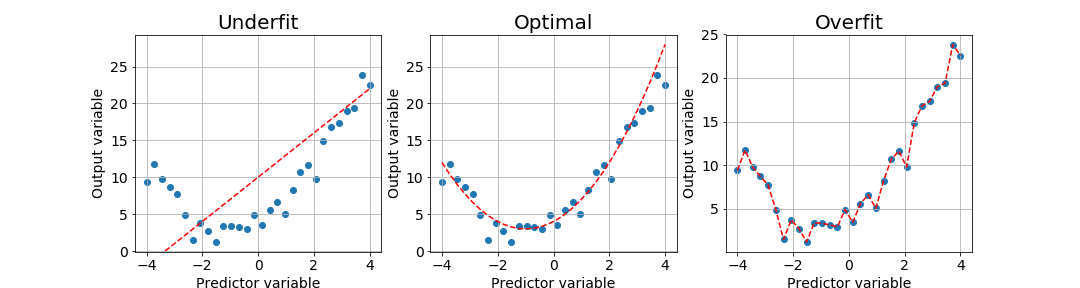
\includegraphics[scale = 0.4]{Chapter3_Method/figs/generalization.png}
%    \caption{Fitting at different levels. The optimal fit is the most general one. This is applicable to many cases. For the traditional autoregressive models, the predictor variable is the true value in the previous time step. }
%    \label{fig:linreg_overfitting}
%\end{figure}

%Its relevant for all ML algorithms but easiest to visualize for linear regression.
%\textit{Overfitting a model is a condition where a statistical model begins to describe the random error in the data rather than the relationships between variables.}

\section{Related work} \label{sec:related_work}
Deep learning is a young field and \acrshort{convlstm} even younger model. Few studies have been conducted within \acrshort{dl} applied to sequence modelling. The task of object detection or classification receives the most attention.

The \acrshort{convlstm} was developed by \citepaper{precip_nowcasting} for the task of precipitation nowcasting. \citepaper{SunAirLSTM} applied it to the air quality forecasting problem. Using high resolution data from a period up to two years. Both studies evaluate their models based on case specific metrics. In other words the performance of these models are not comparable across probelems. \textbf{Vil man egentlig noen gang gjøre det..?}

\citepaper{precip_nowcasting} use gridded data and the spatial dimension is $100\times 100$ after resizing it using filters to remove noise. It is named the radar echo dataset, and have training 8148 sample, 2037 validation and 2037 test samples. Each sample consist of 20 frames, 5 used for input and 15 used for prediction. Based on five frames the model predicts 15. Report that they are training one model $ConvLstm(3\times 3)3\times 3-64-3\times 3-64$, a \acrshort{convlstm} model using a $3\times 3$ filter, in combinations with 64 hidden states, twice. Patch size is 2, this is compared to a FC-LSTM-2000-2000 and a traditional model for precipitation nowcasting, ROVER. Both LSTM version optimise the crossentropy error of 15 prediction samples. 

\citepaper{SunAirLSTM} use a combination of distributed data. Weather data is provided in grids, and air quality observations are point measurements. The weather data volume per time step is a tensor of shape $(21 \times 31 \times 5)$. 16 months of hourly data divided into sequences of 72 frames, 24 for input and 48 for prediction. Batch size is not mentioned in the paper, but based on Figure X, where one tensor of shape $(21 \times 31 \times 5)$ is sent as input. i.e. one sample. They use a learning rate scheduler dropping from 0.01 to 0.001 after five epochs. Gradient clipping to avoid exploding gradients when training longer sequences. Combinations of filters $1\times 1$, $3\times 3$ and $5\times 5$. Two or three layers with either 256 or 128 hidden states, in more familiar terms the number of filters applied. The model names is given following this structure, described using a example. The model \textit{ConvLSTM 3x3-256-2}, is a \acrshort{convlstm} model using a $3\times 3$ filter, 2 layers having the same number hidden states, 256.
\begin{enumerate}[noitemsep, topsep=0pt]
    \item ConvLSTM 1x1-256-2
    \item ConvLSTM 3x3-256-2
    \item ConvLSTM 5x5-256-2
    \item ConvLSTM 3x3-256-3
    \item ConvLSTM 5x5-256-3
\end{enumerate}

Include patch size of 4 making 64x64 to 16x16x16 tensors. Choice of optimizer is RMSprop 0.001 and a learning rate decay of 0.9. Performs early stopping on the validation set.

Filter 1x1 result in the state-to-state transitions.

%%%%%%%%%%%%%% above here is ok

%In this works the model is trained on a small amount of data. Unlike like dataset.
%State-of-the art models 

 


%%%% summarize precipitation nowcasting 



%%%%%%%%%%% summarize the 

%A hyper parameter is a constant set before the training procedure begins. There is a mind-boggling amount of choices for hyperparameters, the initial configuration used in the conducted experiments for this project draw inspiration from this paper. 

%Deep learning is a young field and not many studies have been conducted in the intersection with geosciences. This section provide a brief introduction to some relevant studies and their findings. 

\cleardoublepage

\chapter{Dataset - European Cloud Cover }
%This chapter presents the developed methodology used in the compilation of the dataset. 
This section presents the developed algorithms necessary for the compilation of the dataset \acrfull{ecc}. It is pieced together from two sources, ERA5 reanalysis and \acrlong{msg} cloud mask.

Several candidate satellites were studied before arriving at the combination of datasets presented in this chapter. Spatiotemporal consistency and resolution were given high priority. The variable cloud mask is provided by many satellites, bringing valuable information in itself, but also for the retrieval of other variables restricted to cloud free conditions, such as humidity. The satellite product chosen for this project is the \acrfull{msg}. This satellite is in geostationary orbit, and has an exceptional temporal resolution, scans every 15min. Knowing that the average lifetime of a cloud is 60min or less, it seems like a reasonable choice (\cite{lohmann2016}, pp. 19). The finished dataset, described in detail below, is named \acrfull{ecc}.

\section{Domain}
The geographical domain has, for this project, been restricted to latitude, $\theta \in[30,50]$ and longitude $\phi \in [-15, 25]$. The resulting dimensions of the grid become $81\times161$ pixels. Figure \ref{fig:map} shows the domain included in this dataset. The domain covers central Europe and north Africa.
\begin{figure}[h]
    \centering
    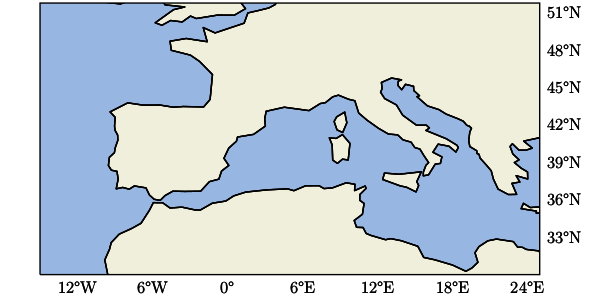
\includegraphics[scale = 1.0]{python_figs/Domain.png}
    \caption[Map over domain.]{Map showing the domain in the projection available in \acrshort{ecc}.}
    \label{fig:map}
\end{figure}

\section{Physical basis of variable decision} \label{sec:ecc}
The overall goal is to investigate whether basic meteorological variables such as temperature, pressure and humidity are sufficient for prediction of cloud fractional cover with a reasonable accuracy. As discussed in Section \ref{sec:cloud_in_climate_system}, cloud dynamics is far more complicated than what can be describes by these variables. 
What is believed to be a sufficiently accurate model is further explained in Chapter \ref{ch:computer_experiments}.

%Reasonable accuracy can mean so much and it is different based on the method of evaluation and the chosen metric. A parametrization can be evaluated in isolation or in the context of a \acrshort{esm}-model. 
%There are several options when determining what is sufficiently accurate, a method can be evaluated in isolation and in the context of a climate model. In isolation it should be better than a a benchmark (chosen by ??) and in the context of a climate model it would be reducing the spread of uncertainty related to the variable we are predicting. 

This project is a \textit{proof of concept study} aimed to demonstrate the feasibility of using \acrshort{ai} to parametize \acrshort{cfc}. Employing data driven learning to represent cloud physics and dynamics in its full complexity requires measurements from technologies not yet invented. If they did exist, the computational cost would be enormous, and even then there would be no guarantee that the model performance would be %\textcolor{red}{the?} 
state-of-the-art.
%Not feasible in the foreseeable future to incorporate all the effects of micro-physics at a sufficient accuracy. 

Macrophysics properties describes the cloud as a unit, using properties like base height, top height, thickness, fractional cover and regime (also known as type). Microphysical processes are all mechanisms involving the particles forming a cloud. Examples of properties used to quantify the microphysical state
%\textcolor{red}{Synes "making up" a cloud hørtes litt rart ut, men det er du som er skyeksperten. Ville vurdert en annen beskrivelse hvis du har}. Examples of these variable \textcolor{red}{I setningen før har du kalt det for microphysical processes som er alle mechanisms. ville da også vurdert å bruke det videre "Examples of these mechanisms/microphysiacal processes are...." og evt. " and is treated as variables in the model/study" eller noe lignende} 
are \acrshort{ccn} and droplet number concentrations (\cite{Grabowski2019ModelingBetter}). Precipitation formation and cloud optical thickness are affected by changes on a microphysical level. However, they are undeniably closely related to the macrophysical properties of the cloud. Imagine precipitation without a cloud fractional cover? 

Reliable estimates of large-scale variables are available from using reanalyse or other climate models. Restricting the focus to the macrophysical aspect of clouds  makes it reasonable to chose these as explanatory variables and thereby ensuring that it is possible to build usable application of this parameterization in the future.

%Focusing on the macrophysical aspect of clouds its is reasonable to chose large-scale variables \textcolor{red}{Rar setning. gir ingen mening å bruke "its". Mener du kanskje "Focusing on the macro-physical aspect of clouds, it is reasonable to chose large-scale variables,..."}, for which reliable estimates are available from using reanalyse or other climate models, thereby ensuring that it is possible to build usable application of this in the future. \textcolor{red}{ALTFOR lang setning. Hele avsnittet er en setning! }
%\textcolor{red}{Focusing on the macro-physical aspect of clouds, it is reasonable to chose large-scale variables. Because, reliable estimates are available from the use of reanalyse or other climate models. It then ensures that it is possible to build usable application of this (hva er this? the variables?) in the future.}
For this dataset, all variables are produced by ERA5. Some variables have been chosen because they are reliable and fundamental meteorological variables, e.g. temperature and surface pressure. Others because they are essential in cloud formation, e.g. specific and relative humidity. They are all retrieved from the surface or the closest pressure level (1000hPa). This following section gives a brief introduction to their role in cloud formation. %\textcolor{red}{(Nå er du midt i seksjonen, så føles litt rart at du kommer med dette her, men kan kanskje heller si at "the rest of the section gives a brief ...."}

From the weather maps on the news, low and high pressure systems might be familiar terms. Low pressure systems are often associated with precipitation, while high pressure systems are associated with nice weather. The earth is not equally heated due to the earths spherical geometry. Warmer air rises, generating a low pressure at the surface. As the air rises the temperature decreases. From Equation \eqref{eq:clausius_clapeyron} it can be shown that, colder air can retain less vapour, enhancing the rate at which saturation is achieved. Under supersaturated conditions some of the vapour condenses, generating cloud water, forming a cloud, and occasionally precipitation. Summer is often associated with convective motions generating cumulus type clouds. %Evaporation rates 
%In presence of water at the surface, evaporation rates are also higher in a warmer climate \textcolor{red}{eller ikke? Fordamping drives vel av forskjellen i luftfuktighet ved bakken og luften i tillegg til vind? SElv om det er veldig varmt, men høy luftfuktighet så vil du ha lite fordamping. Så drivkraften er ikke varme. Tror ligningen er noe som fordamping = (e-es)*u hvor e er vannmetning i lufta og es ved overflaten eller noe og u er vind (men dette er tatt ut av hukommelsen og jeg ville sjekket det i Dingman)}. \textcolor{red}{Ellers et veldig bra avsnitt! Tydelig og enkelt forklart på en bra måte}

In areas of lower pressure, the surrounding air will flow toward the low pressure centre to offset the pressure difference. Induced by earths rotation the Coriolis effect force winds of low pressure system to swirl counterclockwise north of the equator and clockwise south of the equator, causing an accumulation of air in the centre of low pressure system. Pushing it to higher altitudes in the atmosphere. A high pressure system exhibit the exact opposite behaviour, it swirls in the reverse direction, and the air flows from the centre. Diverging air masses cause sinking motions of parcels from higher in the atmosphere to fill the void. 
% air from higher in the atmosphere to sink and fill the space left.
% \textit{Air from higher in the atmosphere sinks down to fill the space left as air moves outward.} 
Winds transports the substances suspended in air, such as pollutants and humidity. 

The dataset includes both relative and specific humidity. Relative humidity is a measure of how much vapour the air contains, relative to how much it can hold at a certain temperature. At relative humidity of 1 the air is at its dew point, and for higher values clouds form, under such supersaturated conditions it is often referred to as \textbf{X}, and therefore it is common to limit the range of relative humidity to be between 0 and 1. However the variable is still a measure of the identical ratio, and this explains why values exceeding 1 is present in the dataset. Relative humidity is unitless and for higher values the air is more humid.

Specific humidity is the ratio between mass of vapour and mass of air, with unit of $kg kg^{-1}$ (\cite{lohmann2016}, pp. 53-54). Whether the relative or specific humidity is the better predictor is not clear a priori. The data is gathered from the model level closest to the surface, at an altitude of 1000hPa (\cite{lohmann2016}, pp. 81-84). 

\section{Area Weighting Regridding Scheme (AWRS)} \label{sec:remapping}
Computing cloud fractions based on cloud mask requires a regridding scheme. Common schemes for solving similar tasks are mean, nearest neighbour or area weighting. For this particular task, the pixels are of uneven size and the area weighted scheme seemed most appropriate. 

This section provides a step-by-step description of the necessary data processing done for the compilation of \acrshort{ecc}, transforming clouds masks provided in \textit{space-view} to cloud fractions on a uniform grid. \acrshort{eumetsat} doesn't provide suitable software to tackle this particular task (personal communication EUMETSAT staff). Building the dataset requires the implementations of software with functionality to perform the regridding, described in detail below and named the \acrfull{awrs}.

The regridding algorithm consist of two modules; \textit{detection algorithmn} and \textit{the area weighting}. Let the subscripts denote the dataset pertaining to a particular grid. Grid\textsubscript{MSG} refers to the space-view grid of the \acrlong{msg} and grid\textsubscript{ECC} refers to the uniform grid originating from ERA5. Note that the grid\textsubscript{ECC} is identical to  grid\textsubscript{ERA5}. The \textit{detection algorithmn}, determines the contributing pixel from grid\textsubscript{MSG} 
to the particular cells in the other coordinate system,
grid\textsubscript{ERA5} 
and their classification into the different categories such as \textit{corner}, \textit{centre}, \textit{left}, \textit{right}, \textit{upper} and \textit{lower boundary}. These categories are later used to isolate the portion of the pixel contributing to grid\textsubscript{ECC}.
%This is necessary to compute the area of the overlapping pixels. 
%\textbf{Include somewhere? In order to compute the area of the boundary pixels, their centre need to be rectified to the centre of the subsection that fall within the boundaries of grid\textsubscript{ECC}, and the pixel extent need to be updated.}
The second module, \textit{the area weighting}, consist of the category based area weighting algorithm based on the developed equations.

\subsection{Deriving Grid Area}
Assuming a spherical earth, pixel-areas are therefore computed using spherical coordinates. Figure \ref{fig:spherical_coords} shows a square projected on to a sphere. Deriving the equation for computing the area of a square in spherical coordinates, requires integrating over changes in latitude, $d\theta$ and longitude, $d\phi$. In Equation \eqref{eq:sphere_integral} the variables of integration is given a prime to keep them distinct from the integration boundaries.
\begin{figure}
    \centering
    
    
\tdplotsetmaincoords{60}{110}
%
\pgfmathsetmacro{\rvec}{1.0}
\pgfmathsetmacro{\thetavec}{30}
\pgfmathsetmacro{\phivec}{60}

\pgfmathsetmacro{\deltathetavec}{40}
\pgfmathsetmacro{\deltaphivec}{80}

%
\begin{tikzpicture}[scale=5,tdplot_main_coords]
    \coordinate (O) at (0,0,0); % origo

    \coordinate (z) at (0, 0, 1.0); % origo
    %\draw[thin, <->] (1, 0.7, 1.16) -- (1, 0.52, 1.2) node[pos = 0.8, above right]{\Large $d\theta$};
    
    \draw[very thick,->] (0,0,0) -- (1.7, 0, 0) node[anchor=north east]{\Large $x$};
    \draw[very thick,->] (0,0,0) -- (0, 1.7, 0) node[anchor=north west]{\Large $y$};
    \draw[very thick,->] (0,0,0) -- (0, 0, 1.7) node[anchor=south]{\Large $z$};
    \shade[ball color = teal, opacity = 0.1] (0,0,0) circle [radius=\rvec];
    \draw (0,0,0) circle [radius=\rvec];
    
    \tdplotsetcoord{P}{\rvec}{\thetavec}{\phivec}
    \tdplotsetcoord{dP}{\rvec}{\deltathetavec}{\phivec}
    
    \tdplotsetcoord{G}{\rvec}{\thetavec}{\deltaphivec}
    \tdplotsetcoord{dG}{\rvec}{\deltathetavec}{\deltaphivec}

    \draw[very thick, color=teal, opacity = 0.3] (O) -- (G) node[above right]  {};
    \draw[very thick, color=teal, opacity = 0.6] (O) -- (dG) node[above right] {};    
    \draw[very thick, color=red, opacity = 0.6] (O) -- (P) node[above left]  {\Large $R$};
    \draw[very thick, color=teal, opacity = 0.6] (O) -- (dP) node[above right] {};
    
    \draw[dashed, color=teal] (O) -- (Pxy);
    \draw[dashed, color=teal] (dP) -- (Pxy);
    %\draw[dashed, color=red] (Pz) -- (Py);

    %\draw[dashed, color=red] (dP) -- (Pxy);
    
    \draw[very thick, color=red] (O) -- (Gxy) node[above right] {\Large $Rcos\theta$};
    \draw[dashed, color=teal] (dG) -- (Gxy);
    %\draw[dashed, color=black,looseness = 10, bend left] (z) -- (G)  node[pos = 0.6, above right] {\Large $Rsin\theta$};
    \draw[dashed, color=teal,looseness = 10, bend left] (z) -- (G);
    \draw[dashed, color=teal, bend right] (P) -- (z);
    
    
    \draw [very thick, color=blue] (\phivec:0.5)  arc (\phivec:\deltaphivec:0.5) node [below right, pos=0.3] {\Large $Rcos\theta d\phi$};

    
    %\tdplotdrawarc[tdplot_rotated_coords, ->]{(dP)}{.7}{(Pxy)}
    
    \draw[dashed, very thick, color=teal, fill = teal, opacity = 0.2] (P) -- (dP) -- (dG) -- (G) -- (P);
    \draw[dashed, very thick, color=teal] (P) -- (dP) -- (dG) -- (G) -- (P);
    \draw[very thick, color=blue] (dG) -- (G) node[pos = 0.5, above right] {\Large $Rd\theta$};
    \draw[dashed, color=teal] (dG) -- (G);    \tdplotdrawarc[]{(O)}{0.4}{0}{\phivec}{anchor=north}{\Large $\phi$}
    %\tdplotdrawarc{(O)}{0.2}{0}{\deltathetavec}{anchor=north}{$\theta$}

    \tdplotsetthetaplanecoords{\phivec};
    
    %\tdplotdrawarc[tdplot_rotated_coords]{(0,0,0)}{0.8}{0}%
        %{\thetavec}{anchor=south west}{\Large $\theta$};
    
    \tdplotdrawarc[tdplot_rotated_coords, pos = 0.01]{(0, 0.5, -0.3)}{0.45}{0.0}%
        {\thetavec}{anchor=south west}{\Large $\theta$};
    
    \tdplotdrawarc[tdplot_rotated_coords, pos = 0.5]{(0,0,0.2)}{0.26}{0}%
        {\thetavec}{anchor = south west,shift={(4mm,-5mm)}}{\Large $d\theta$};
        
    %\tdplotdrawarc[tdplot_rotated_coords, <->]{(0.1, 0.2, 0)}{.5}{0}{\thetavec}{anchor=east}{\Large $d\theta$}
    \shade[ball color=teal,tdplot_screen_coords,opacity=0.1] (O) circle[radius=\rvec];
    \foreach \X/\Y in {xy/z,yz/x,zx/y}
        {\begin{scope}[canvas is \X\space plane at \Y=\rvec]
         \fill circle[radius=1pt];
        \end{scope}}
    \end{tikzpicture}
    \caption{Properties of a square in spherical coordinates.}
    \label{fig:spherical_coords}
\end{figure}
The general expression for the area of a square in spherical coordinates, is given by the following integral,
\begin{equation} \label{eq:sphere_integral}
    A = R^2\int_{ \theta - \delta \theta }^{\theta + \delta \theta} \int_{ \phi - \delta \phi }^{\phi + \delta \phi} cos\left( \theta' \right) d\phi' d\theta'
\end{equation}
%This can be rewriting into, \textbf{needs indices $(i, j)$ ..?}
rewriting the equation into
\begin{equation} \label{eq:sphere_finish}
    A \left( \theta, \phi, \delta \theta, \delta \phi   \right)= 2R^2 \left( sin\left( \theta + \delta \theta  \right) - sin\left(  \theta - \delta \theta  \right) \right) \delta \phi
\end{equation}
where $R=6378km$ denotes the distance to earths centre, $\theta$ the latitude and $\phi$ the longitude. Relating Equations \eqref{eq:sphere_integral} and \eqref{eq:sphere_finish} to Figure \ref{fig:spherical_coords} by setting $d \theta = 2 \delta \theta$ and $d \phi = 2 \delta \phi$. The implementation is scaled by $R$.

The equations used to compute the area weighted cloud fractional cover is as follows,
\begin{equation} \label{eq:area_weighting}
    CFC_{ECC} = \frac{1}{A} \sum_{i=0}^{N} a_i m_i
\end{equation}
where,
\begin{equation} \label{eq:tot_area}
    A = \sum_{i=0}^{N} a_i
\end{equation}
Inserting $m_i = 1$ $\forall$ $i \in [0,N]$ into Equation \eqref{eq:area_weighting} results in $CFC_{ECC}=1$, independent of $a_i$, proving that the minor overlap between pixels in Figure \ref{fig:pixels_contributing_to_cell} doesn't affect the range of cloud fractions, which remains between 0 and 1.

\subsection{Estimating extent}
% Estimating the extent of the cell.
The coordinate information is provided in grids of latitudes, $\theta$ (degrees north), and longitudes, $\phi$ (degrees east) values. The coordinate represent the centre of a pixel. To acquire the information about the extent of cells in a non-uniform grid require some simplifications. 

%%%%%%%%%%%%% PART ONE
Computing the area weighted average of cloud masks requires detecting the grid\textsubscript{MSG}
contributing to the grid\textsubscript{ERA5} cell, and computing their area. The pixels are classified into five categories; \textit{centre}, \textit{left}, \textit{right}, \textit{up} and \textit{down boundary}.
%The detection algorithm is straight forward, overlapping pixels are included and labelled with a suitable category.
The cloud mask pixels are smallest at the nadir point, decreasing in all directions. Figure \ref{fig:estimate_dlon} illustrates this by showing an example of three neighbouring pixels. In this example the apparent pixel size increases going eastward. Consequently, there is an asymmetry between neighbouring pixels. The distance from the centre to the right and left neighbour is unequal. In order to take advantage of the analytical expression derived in Equation \eqref{eq:sphere_finish}, the extent of a contributing pixel is approximated by averaging the right and left distances. The categorisation is illustrated in Figure \ref{fig:pixels_contributing_to_cell} using different colours.

\tdplotsetmaincoords{60}{110}
%
\pgfmathsetmacro{\rvec}{1.6}
\pgfmathsetmacro{\thetavec}{30}
\pgfmathsetmacro{\phivec}{60}

\pgfmathsetmacro{\deltathetavec}{40}
\pgfmathsetmacro{\deltaphivec}{80}

\begin{figure}
    \centering
    
    
\tdplotsetmaincoords{60}{110}
%
\pgfmathsetmacro{\rvec}{1.0}

\pgfmathsetmacro{\thetavec}{30}
\pgfmathsetmacro{\deltathetavec}{40}
\pgfmathsetmacro{\deltatwothetavec}{50}
\pgfmathsetmacro{\deltathreethetavec}{60}

\pgfmathsetmacro{\phivec}{-30}
\pgfmathsetmacro{\deltaphivec}{10}
\pgfmathsetmacro{\deltatwophivec}{50}
\pgfmathsetmacro{\deltathreephivec}{90}



\begin{tikzpicture}[scale=5,tdplot_main_coords, 
                    mycirc/.style={circle,fill=blue!20, minimum size=0.5cm}]

    %%%%%%%%%%%%%% Setting up axis and coordinate system.
    \coordinate (O) at (0,0,0); % origo
    \coordinate (z) at (0, 0, \rvec); % origo
    %\draw[thin, <->] (1, 0.7, 1.16) -- (1, 0.52, 1.2) node[pos = 0.8, above right]{\Large $d\theta$};
    \draw[very thick,->, opacity = 1.] (0,0,0) -- (1.7, 0, 0) node[anchor=north east]{\Large $x$};
    \draw[very thick,->,  opacity = 1.] (0,0,0) -- (0, 1.7, 0) node[anchor=north west]{\Large $y$};
    \draw[very thick,->,  opacity = 1.] (0,0,0) -- (0, 0, 1.7) node[anchor=south]{\Large $z$};
    \shade[ball color = teal, opacity = 0.1] (0,0,0) circle [radius=\rvec];
    \draw (0,0,0) circle [radius=\rvec];

    
    \tdplotsetcoord{a}{\rvec}{\deltathetavec}{\phivec}
    \tdplotsetcoord{b}{\rvec}{\deltatwothetavec}{\phivec}
    % Changeing the rightmost part 
    \tdplotsetcoord{c}{\rvec}{\deltathetavec-5}{\deltaphivec}
    \tdplotsetcoord{d}{\rvec}{\deltatwothetavec+5}{\deltaphivec}
    
    \draw[dashed, very thick, color=teal, fill = teal, opacity = 0.2] (a) -- (b) -- (d)-- (c) -- (a);
    \draw[dashed, very thick, color=teal] (a) -- (b) -- (d)-- (c) -- (a);

    \tdplotsetcoord{a}{\rvec}{\deltathetavec-5}{\deltaphivec}
    \tdplotsetcoord{b}{\rvec}{\deltatwothetavec+5}{\deltaphivec}
    \tdplotsetcoord{c}{\rvec}{\deltathetavec-10}{\deltatwophivec}
    \tdplotsetcoord{d}{\rvec}{\deltatwothetavec+10}{\deltatwophivec}
    
    \draw[dashed, very thick, color=teal, fill = teal, opacity = 0.2] (a) -- (b) -- (d)-- (c) -- (a);
    \draw[dashed, very thick, color=teal] (a) -- (b) -- (d)-- (c) -- (a);
        
    % First column
    %\node[draw] at (0, -2)  (c)     {C};
    %\node[draw] at (0.3, -0.25, 0.5) {$\phi_{(i,j-1)}$};
    %\node[draw, thick] at (0.5, 0.3, 0.65) {$\phi_{(i,j)})$};
    %\node[draw, thick] at (0.5, 0.73, 0.87) {$(i,j+1)$};
    \filldraw [teal, label=above:{$\phi_{(i,j-1)}$}]  (0.3, -0.25, 0.5) circle (1pt);
    \filldraw [teal, label=above:{$\phi_{(i,j-1)}$}]  (0.5, 0.3, 0.65)  circle (1pt);
    \filldraw [teal, label=above:{$\phi_{(i,j-1)}$}]  (0.5, 0.73, 0.87) circle (1pt);
    
    \tdplotsetcoord{a}{\rvec}{\deltathetavec-10}{\deltatwophivec}
    \tdplotsetcoord{b}{\rvec}{\deltatwothetavec+10}{\deltatwophivec}
    \tdplotsetcoord{c}{\rvec}{\deltathetavec-15}{\deltathreephivec}
    \tdplotsetcoord{d}{\rvec}{\deltatwothetavec+15}{\deltathreephivec}
    
    \draw[dashed, very thick, color=teal, fill = teal, opacity = 0.2] (a) -- (b) -- (d)-- (c) -- (a);
    \draw[dashed, very thick, color=teal] (a) -- (b) -- (d)-- (c) -- (a);
    
    \draw [decorate,decoration={brace, amplitude=12pt, mirror}, xshift=0pt, yshift=0pt]
    (0.3, -0.25, 0.1) -- (0.5, 0.83, 0.47) node [black,midway,xshift=0.2cm, yshift = -1.5cm, very thick] {\Large $\left| \phi_{i+1,j} - \phi_{i-1, j} \right| $};
    
    \draw [decorate,decoration={brace, amplitude=12pt}, xshift=0pt, yshift=0pt]
    (0.5, 0.3, 0.65) -- ((0.5, 0.5, 0.73) node [black,midway,xshift=0cm, yshift = 2.cm, very thick] {\Large $\delta \phi_{(i, j)}$};

    \tdplotsetthetaplanecoords{\phivec};
    \shade[ball color=teal,tdplot_screen_coords,opacity=0.2] (O) circle[radius=\rvec];
    \foreach \X/\Y in {xy/z,yz/x,zx/y}
        {\begin{scope}[canvas is \X\space plane at \Y=\rvec]
         \fill circle[radius=1pt];
        \end{scope}}
    \end{tikzpicture}
    
    \caption{Illustrating the relative size of three neighbouring pixels on a sphere in the \textit{space-view} grid provided by EUMETSAT. The following example explain the changes in longitude, $\phi$, varying in eastward direction, denoted $i$. The expression is shown in Equation \eqref{eq:app_lon}. 
    The same principles applies in the latitudinal direction, see Equation \eqref{eq:app_lat}.  }
    \label{fig:estimate_dlon}
\end{figure}

\begin{figure}
    \centering
    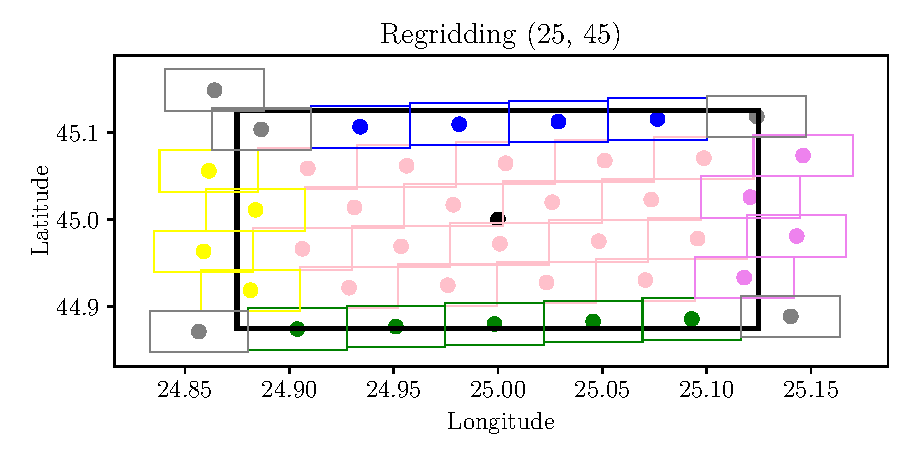
\includegraphics{python_figs/example_remapping_lat45_lon25.pdf}
    \caption{Example showing the contributing pixels to the remapping of pixel $(25, 45)$. The pixels from the satellite is classified into corner (grey), centre (pink), right (purple), left (yellow), down (green) and up (blue) boundary. The dense black line is the pixel in grid\textsubscript{ECC}, and the other pixels shows the contributing pixels from grid\textsubscript{MSG}.}
    \label{fig:pixels_contributing_to_cell}
\end{figure}

Approximation of $d\phi$ and $d\theta$ have been done based on the two-dimensional fields of latitude and longitude values according to the below equations.
Longitudinal values vary along the first dimension, denoted with index i. The estimated half the extent of a pixel in grid\textsubscript{MSG} is approximated by Equation \ref{eq:app_lon}. Latitudinal changes are in north-south direction, along the second-axis, here denoted with index, j. Equation \eqref{eq:app_lat} describes the distance from the centre to the upper and lower boundary.
% \eqref{eq:app_lon} and  \eqref{eq:app_lat}. 
%The horizontal extent of a pixel $(i,j)$ be determined by the the averaged distance between the longitude of neighbouring pixels. 
%, see Equation \eqref{eq:app_lon}. The same principles applies in the latitudinal direction, this version is shown in Equation \ref{eq:app_lat}.
\begin{equation} \label{eq:app_lon}
    \delta \phi_{i,j} = \left| \frac{\phi_{i+1,j} - \phi_{i-1, j}}{4} \right|
\end{equation}
\begin{equation} \label{eq:app_lat}
    \delta \theta_{i,j} = \left| \frac{\theta_{i,j+1} - \theta_{i, j-1}}{4} \right|
\end{equation}

The ``square'' in grid\textsubscript{MSG} resembles trapezium, this is illustrated in Figure \ref{fig:estimate_dlon}. As far as the author know, it doesn't exist an analytical solution to an area of a trapezium in spherical coordinates. Also, it is not clear if approximating the area with another numerical method would reduce the overall uncertainty. However, it would most likely increase the computational time. \tdplotsetmaincoords{60}{110}
%
\pgfmathsetmacro{\rvec}{1.6}
\pgfmathsetmacro{\thetavec}{30}
\pgfmathsetmacro{\phivec}{60}

\pgfmathsetmacro{\deltathetavec}{40}
\pgfmathsetmacro{\deltaphivec}{80}

\begin{figure}
    \centering
    
    
\tdplotsetmaincoords{60}{110}
%
\pgfmathsetmacro{\rvec}{1.0}

\pgfmathsetmacro{\thetavec}{30}
\pgfmathsetmacro{\deltathetavec}{40}
\pgfmathsetmacro{\deltatwothetavec}{50}
\pgfmathsetmacro{\deltathreethetavec}{60}

\pgfmathsetmacro{\phivec}{-30}
\pgfmathsetmacro{\deltaphivec}{10}
\pgfmathsetmacro{\deltatwophivec}{50}
\pgfmathsetmacro{\deltathreephivec}{90}

\begin{tikzpicture}[scale=5,tdplot_main_coords]

    %%%%%%%%%%%%%% Setting up axis and coordinate system.
    \coordinate (O) at (0,0,0); % origo
    \coordinate (z) at (0, 0, \rvec); % origo
    %\draw[thin, <->] (1, 0.7, 1.16) -- (1, 0.52, 1.2) node[pos = 0.8, above right]{\Large $d\theta$};
    \draw[very thick,->, opacity = 1.] (0,0,0) -- (1.7, 0, 0) node[anchor=north east]{\Large $x$};
    \draw[very thick,->,  opacity = 1.] (0,0,0) -- (0, 1.7, 0) node[anchor=north west]{\Large $y$};
    \draw[very thick,->,  opacity = 1.] (0,0,0) -- (0, 0, 1.7) node[anchor=south]{\Large $z$};
    \shade[ball color = teal, opacity = 0.1] (0,0,0) circle [radius=\rvec];
    \draw (0,0,0) circle [radius=\rvec];

    %%%%%%%%%%%%%%%%%%%%%%%%%%%% first column
    \tdplotsetcoord{P}{\rvec}{\thetavec}{\phivec}
    \tdplotsetcoord{dP}{\rvec}{\deltathetavec}{\phivec}
    \tdplotsetcoord{G}{\rvec}{\thetavec}{\deltaphivec}
    \tdplotsetcoord{dG}{\rvec}{\deltathetavec}{\deltaphivec}
    
    \draw[dashed, very thick, color=teal, fill = teal, opacity = 0.2] (P) -- (dP) -- (dG) -- (G) -- (P);
    \draw[dashed, very thick, color=teal] (P) -- (dP) -- (dG) -- (G) -- (P);
    
    \tdplotsetcoord{a}{\rvec}{\deltathetavec}{\phivec}
    \tdplotsetcoord{b}{\rvec}{\deltatwothetavec}{\phivec}
    \tdplotsetcoord{c}{\rvec}{\deltathetavec}{\deltaphivec}
    \tdplotsetcoord{d}{\rvec}{\deltatwothetavec}{\deltaphivec}
    
    \draw[dashed, very thick, color=teal, fill = teal, opacity = 0.2] (a) -- (b) -- (d)-- (c) -- (a);
    \draw[dashed, very thick, color=teal] (a) -- (b) -- (d)-- (c) -- (a);
    
    \tdplotsetcoord{e}{\rvec}{\deltatwothetavec}{\phivec}
    \tdplotsetcoord{f}{\rvec}{\deltathreethetavec}{\phivec}
    \tdplotsetcoord{g}{\rvec}{\deltatwothetavec}{\deltaphivec}
    \tdplotsetcoord{h}{\rvec}{\deltathreethetavec}{\deltaphivec}
    
    \draw[dashed, very thick, color=teal, fill = teal, opacity = 0.2] (e) -- (f) -- (h)-- (g) -- (e);
    \draw[dashed, very thick, color=teal] (e) -- (f) -- (h)-- (g) -- (e);

    %%%%%%%%%%%%%%%%%%%%%%%%%%%%%%%% second column
      
    \tdplotsetcoord{P}{\rvec}{\thetavec}{\deltaphivec}
    \tdplotsetcoord{dP}{\rvec}{\deltathetavec}{\deltaphivec}
    \tdplotsetcoord{G}{\rvec}{\thetavec}{\deltatwophivec}
    \tdplotsetcoord{dG}{\rvec}{\deltathetavec}{\deltatwophivec}
    
    \draw[dashed, very thick, color=teal, fill = teal, opacity = 0.2] (P) -- (dP) -- (dG) -- (G) -- (P);
    \draw[dashed, very thick, color=teal] (P) -- (dP) -- (dG) -- (G) -- (P);
  
      
    \tdplotsetcoord{a}{\rvec}{\deltathetavec}{\deltaphivec}
    \tdplotsetcoord{b}{\rvec}{\deltatwothetavec}{\deltaphivec}
    \tdplotsetcoord{c}{\rvec}{\deltathetavec}{\deltatwophivec}
    \tdplotsetcoord{d}{\rvec}{\deltatwothetavec}{\deltatwophivec}
    
    \draw[dashed, very thick, color=teal, fill = teal, opacity = 0.2] (a) -- (b) -- (d)-- (c) -- (a);
    \draw[dashed, very thick, color=teal] (a) -- (b) -- (d)-- (c) -- (a);
  
  
    \tdplotsetcoord{e}{\rvec}{\deltatwothetavec}{\deltaphivec}
    \tdplotsetcoord{f}{\rvec}{\deltathreethetavec}{\deltaphivec}
    \tdplotsetcoord{g}{\rvec}{\deltatwothetavec}{\deltatwophivec}
    \tdplotsetcoord{h}{\rvec}{\deltathreethetavec}{\deltatwophivec}
    
    \draw[dashed, very thick, color=teal, fill = teal, opacity = 0.2] (e) -- (f) -- (h)-- (g) -- (e);
    \draw[dashed, very thick, color=teal] (e) -- (f) -- (h)-- (g) -- (e);
    
    
    %%%%%%%%%%%%%%%%%%%%%%%%%%%%%%%% third column
    \tdplotsetcoord{P}{\rvec}{\thetavec}{\deltatwophivec}
    \tdplotsetcoord{dP}{\rvec}{\deltathetavec}{\deltatwophivec}
    \tdplotsetcoord{G}{\rvec}{\thetavec}{\deltathreephivec}
    \tdplotsetcoord{dG}{\rvec}{\deltathetavec}{\deltathreephivec}
    
    \draw[dashed, very thick, color=teal, fill = teal, opacity = 0.2] (P) -- (dP) -- (dG) -- (G) -- (P);
    \draw[dashed, very thick, color=teal] (P) -- (dP) -- (dG) -- (G) -- (P);
  
    \tdplotsetcoord{a}{\rvec}{\deltathetavec}{\deltatwophivec}
    \tdplotsetcoord{b}{\rvec}{\deltatwothetavec}{\deltatwophivec}
    \tdplotsetcoord{c}{\rvec}{\deltathetavec}{\deltathreephivec}
    \tdplotsetcoord{d}{\rvec}{\deltatwothetavec}{\deltathreephivec}
    
    \draw[dashed, very thick, color=teal, fill = teal, opacity = 0.2] (a) -- (b) -- (d)-- (c) -- (a);
    \draw[dashed, very thick, color=teal] (a) -- (b) -- (d)-- (c) -- (a);
  
    \tdplotsetcoord{e}{\rvec}{\deltatwothetavec}{\deltatwophivec}
    \tdplotsetcoord{f}{\rvec}{\deltathreethetavec}{\deltatwophivec}
    \tdplotsetcoord{g}{\rvec}{\deltatwothetavec}{\deltathreephivec}
    \tdplotsetcoord{h}{\rvec}{\deltathreethetavec}{\deltathreephivec}
    
    \draw[dashed, very thick, color=teal, fill = teal, opacity = 0.2] (e) -- (f) -- (h)-- (g) -- (e);
    \draw[dashed, very thick, color=teal] (e) -- (f) -- (h)-- (g) -- (e);
    
    %%%%%%%%%%%%%%%%%%%%%%%%%% Adding coordinate information

    % First column
    \draw[thick](0.3, -0.25, 0.5)node[scale=0.8, rotate = -15]{$(i,j-1)$};
    \draw[thick](0.3, -0.17, 0.7)node[scale=0.8, rotate = -15]{$(i+1,j-1)$};
    \draw[thick](0.3, -0.3, 0.3)node[scale=0.8, rotate = -15]{$(i-1,j-1)$};

    % Second column
    \draw[thick](0.5, 0.3, 0.65)node[scale=0.8, rotate = 5]{$(i,j)$};
    \draw[thick](0.5, 0.3, 0.85)node[scale=0.8, rotate = 5]{$(i+1,j)$};
    \draw[thick](0.5, 0.3, 0.45)node[scale=0.8, rotate = 5]{$(i-1,j)$};
    
    % Third column
    \draw[thick](0.5, 0.73, 0.87)node[scale=0.8, rotate = 35]{$(i,j+1)$};
    \draw[thick](0.5, 0.8, 0.7)node[scale=0.8, rotate = 35]{$(i-1,j+1)$};

    \draw[thick](0.05, 0.45, 0.73)node[scale=0.8, rotate = 35]{$(i+1,j+1)$};

    \tdplotsetthetaplanecoords{\phivec};
    \shade[ball color=teal,tdplot_screen_coords,opacity=0.1] (O) circle[radius=\rvec];
    \foreach \X/\Y in {xy/z,yz/x,zx/y}
        {\begin{scope}[canvas is \X\space plane at \Y=\rvec]
         \fill circle[radius=1pt];
        \end{scope}}
    \end{tikzpicture}
    
    \caption{Sketch to illustrated the relative size of neighbouring pixels in uniform grid of ECC, projected onto spherical coordinates. The areas of pixels in a uniform grid decrease poleward.}
    \label{fig:relative_size_neigbouring_pixels}
\end{figure}
A visual inspection of the relation between both grids is provided in 
Figure \ref{fig:pixels_contributing_to_cell}. Based on the small overlapping areas, it appears to be a reasonable simplification at the latitudes and longitudes of interest. This particular pixel was chosen since the largest overlap is expected in the periphery of grid\textsubscript{ecc}. The inclusion of the boundary pixels involve estimating the ``new'' centre and the extent of the contributing portion, falling within the boundaries of grid\textsubscript{ECC}. Due to the small overlap between contribution pixel, occasionally more than four pixels are classified as corners. For the sake of simplicity the corner pixels where omitted from the calculations of cloud fraction. The omitting of the corner may have caused the circular pattern shown in Figure \ref{fig:area_pixel_signal}. The areas decrease northward as illustrated in Figure \ref{fig:relative_size_neigbouring_pixels}. This again have most likely enlarged the radius of the circular pattern.
\begin{figure}[ht]
    \centering
    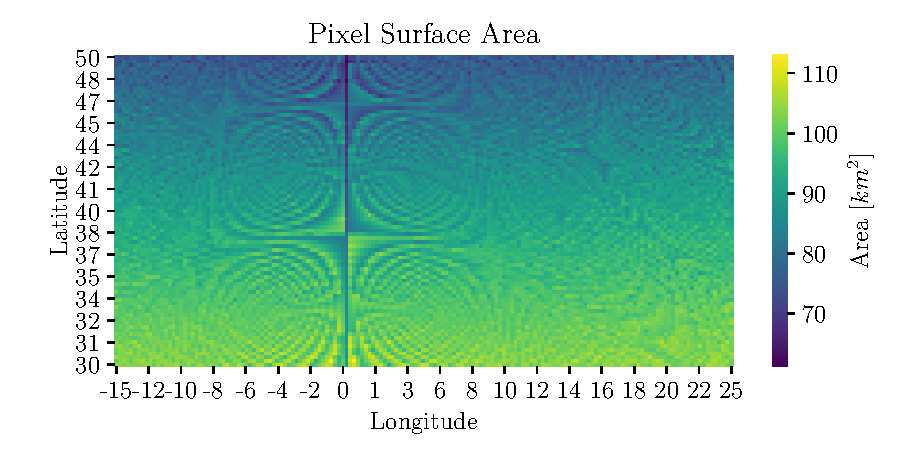
\includegraphics{python_figs/signal_area_pixel.pdf}
    \caption{Illustration of how the areas contributing to a pixel decreases northward. The pattern appear to be more pronounced close to the meridian decreasing in both east and west direction.}
    \label{fig:area_pixel_signal}
\end{figure} 

\section{Verification of AWRS}
The regridding scheme is a set of algorithms. Before the production of the full dataset it is important verify the correctness the algorithms of \acrshort{awrs}.

%%%%%%%%%%%%%%%%%%%%%% TEST 1 - Formula to compute the area 
The computations of the areas are the very foundation of the \acrshort{awrs}, and it it crucial to verify that the algorithm is correct. CDO (\cite{cdo}) provide functionality to compute gridarea using the line inserted below.
\begin{verbatim}
$ cdo gridarea era5data.nc gridarea.nc     
\end{verbatim}
To verify the implementations of Equation \eqref{eq:sphere_finish} the grid areas of ERA5 is computed using both CDO and the self implemented algorithm. They produce the same results.
% må jeg skrive hvor like 
Note that the implementation is scaled by $R$ to be consistent CDO. Multiplication followed by division of the same number provides no additional information, and there is the off chance of introducing additional numerical errors. 

%%%%%%%%%%%%%%%%% TEST 2 -- vis regridding
A reason of confusion in the process of developing the algorithm of the \acrshort{awrs} algorithm arose from the different rotations of the data provided by the \acrshort{grib} and \acrshort{netcdf} files. The coordinate information is availble in \acrshort{netcdf}, but the file-size is to large to store all data in this format, therefore the data is downloaded in \acrshort{grib}, as mention in Section \textbf{X}. The \acrshort{grib}-file is provided as the left and right flipped version of the  \acrshort{netcdf}-file. A fast modular test to check the regridding routine is to insert the raw data including the land and sea masks. Figure \ref{fig:visual_inspection_regridding} shows a example of the regridding of the raw data from 2\textsuperscript{nd} May 2009. Clouds are illustrated in white, land mask in teal and ocean in purple. The original data also include the category off-earth disk, this is not a member of the chosen subset. By regridded the raw data it quickly becomes apparent whether correct domain has been used, and evident if the algorithm generates any discontinuities in space. 
\begin{figure}
    \centering
    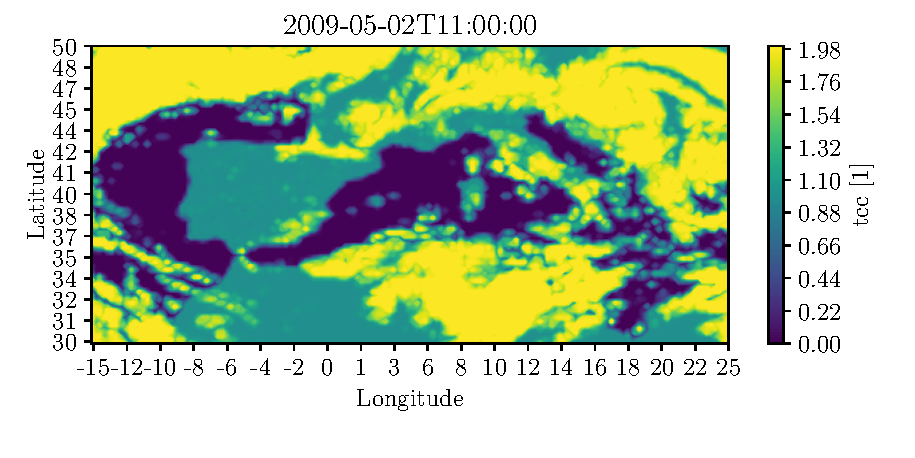
\includegraphics{python_figs/visual_regridding.pdf}
    \caption{Result from regridding raw data, provided with land and sea masks in the absence of clouds. Land is illustrated in teal, ocean in purple and clouds in white.}
    \label{fig:visual_inspection_regridding}
\end{figure}

\section{Missing Data} \label{sec:missing_values}
Missing values is inevitable when working with observational data. Sensors fail to collect measurements and data is missing. This can either be individual pixels or entire disks. In this project single NaN values are no pressing issue since they are remapped to fractions by using the area weighted of the other values. Contributing NaN pixels are counted and stored for future use in \acrshort{ecc}.
\begin{figure}
    \centering
    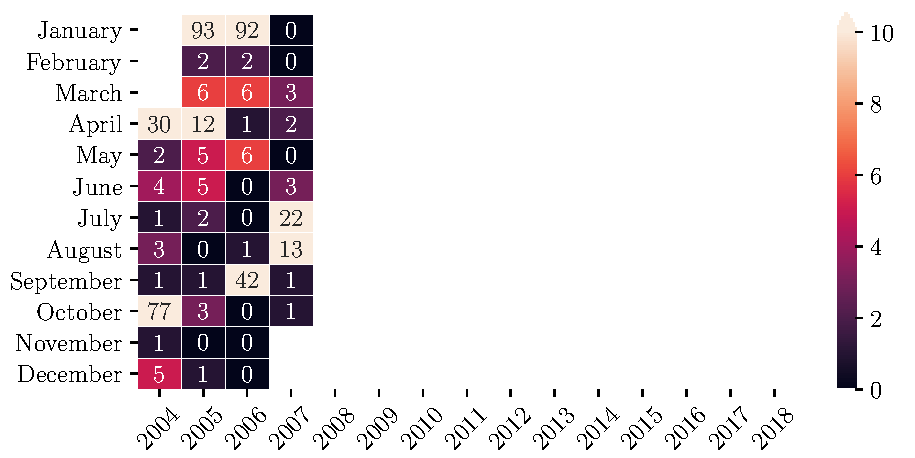
\includegraphics[scale = 1.0]{python_figs/heatmap_missing_values.pdf}
    \caption{Heatmap summarising missing hours per month for all years.}
    \label{fig:heatmap_missing_values}
\end{figure}
\begin{figure}
    \centering
    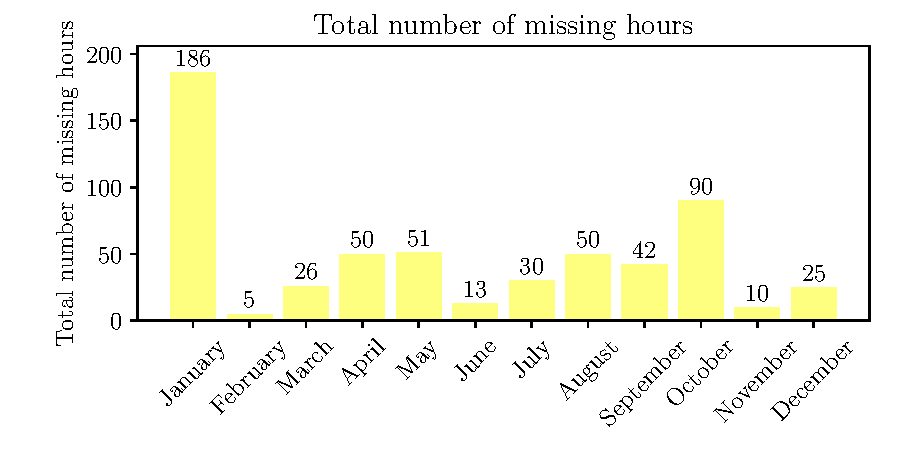
\includegraphics[scale = 1.0]{python_figs/heatmap_missing_values_monthly_sum.pdf}
    \caption{Barplot showing the monthly sum of missing values. This excludes the contribution from the period of 2004 before the satellite was operational.}
    \label{fig:barplot_missing_values}
\end{figure}
In some cases the sensor fail to scan and in other cases the data has been destroyed prior to archiving. The result is the same, the data can never be recovered. Further down the chain of supply, the missing data can cause issues for the process of downloading. Consequently, the requested data has entered infinity loop without being detected by \acrshort{eumetsat}. In combination with the maximum limit of pending request restricted to 20, this has caused some delay. 

The data in each request amount to approximately 3.5 months of hourly data. Missing timestamps, results in missing disks, when available the closest time step within the previous and trailing 45 minutes is used to fill the gap. A summary of missing values per month in the data set is provided in Figure \ref{fig:heatmap_missing_values}. Aggregation of missing values per month is presented in Figure \ref{fig:barplot_missing_values}. The plot is ment to illustrate any seasonal biases. This does not include the months of 2004 prior to the operalization of the satellite.

METeosat provide a two satellite system, occasionally both standby and the operational scan at the same time, as mentioned in Section \ref{sec:meteosat}.
%To reduce the perturbations due to parallax (see Section X) of cloud, given a choice the operational satellite is chosen \textcolor{red}{(skjønte ikke setningen)}. 
In cases over technical failures, the standby scan is used. The scans are done from a different nominal position. However, the coordinate systems remain the same, since the standby scan is rectified to the position of the operational satellite before the product is released (personal communication \acrshort{eumetsat} staff). Comparing simultaneous measurements for the operational and the standby METeosat satellites, it becomes clear that they are disimilar. However, this doesn't occur to frequently and there has been no effort in quantifying the magnitude of the parallax, to correcting for for the bias it may introduce.
% again you have no numbers on the times the standby satellite is used.... 

Manually generated datasets are prone to human error, especially in the case where user need to download individual time steps to fill the gaps. The missing values was were double checked, but there is no guarantee that a few additional time steps is available. In summary the workflow has been as follows, the author downloaded the data, detect missing times and manually choose the closest time step available within the previous and trailing 45 minutes. In retrospect the, the downloading options (API or GUI) provided by the satellite service should be taken into account when choosing the data. A great API can potentially be a large time saver.

\section{Masks} \label{sec:mask}
The land sea masks are regridded from the HTAP-masks provided by \acrfull{metno}. In its original format the HTAP masks have a $0.1^o$ resolution and global coverage, not including the polar regions. These are regridded to a suitable resolution of $0.25^o$ using functionality available in PyAEROCOM (\cite{pyaerocom}). %(\href{https://pyaerocom.met.no/}{https://pyaerocom.met.no/}). 
This is a python toolbox developed within the \acrfull{aerocom} project. To avoid storing redundant data, only domain specific data is made available in the project supplementary repository. For more details on supplementary material, see Section \ref{sec:structure_and_implementations}.
%To keep memory-requirements to a minimum only the parts of the filters relevant domain is stored in the supplementary material for this project.
\begin{figure}
    \centering
    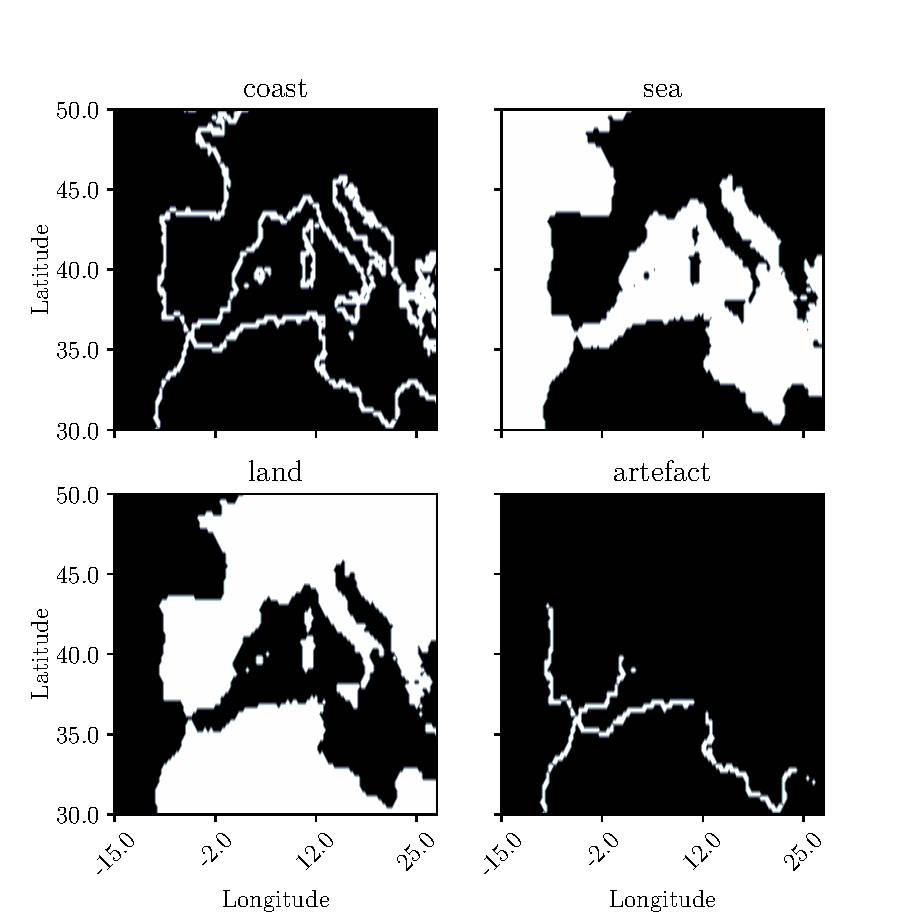
\includegraphics{python_figs/filters.pdf}
    \caption{Figure shows all filters, in white, available in the python package ``sciclouds''.}
    \label{fig:filters_subplot}
\end{figure}

Filters available in the supplementary material are \textit{land}, \textit{sea}, \textit{coastline} and \textit{artefact}. The coastline is defined to be all pixels that are not either 100\% land or sea. A threshold based binary classification is used to separate the coastline pixels into land or ocean. The threshold is set to 50\%. Pixels containing at least 50\% of sea is most likely affected by maritime conditions, making it reasonable to classify them as sea pixels.
\begin{figure}
    \centering
    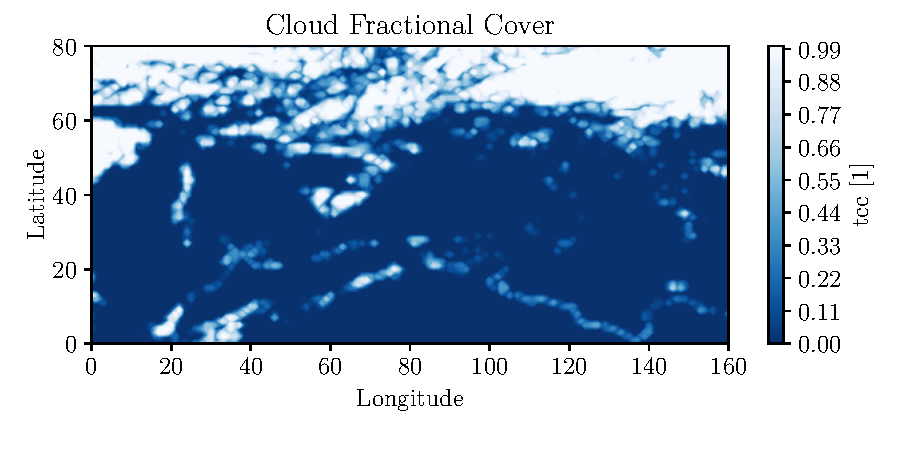
\includegraphics{python_figs/example_artefact.pdf}
    \caption[Artefact in European Cloud Cover dataset.]{The results after regridding revels a artefact. This is a snapshot from May the second 2004 at noon. The frequency of occurrence is currently unknown.}
    \label{fig:example_artefact}
\end{figure}
Based on a visual comparison to Figure \ref{fig:example_artefact}, the artefact is defined to be all coastline pixels obeying the following inequality,  %\eqref{eq:artefact_condition}.
\begin{equation} \label{eq:artefact_condition}
    \theta + \frac{1}{3}\phi < 40
\end{equation}
All filters are displayed in Figure \ref{fig:filters_subplot}. 
%shows a subplot of all filters, including the artefact detecting filter. 
The signal form the artefact filter when applied to \acrshort{ecc} seem to follow a normal distribution as shown Figure \ref{fig:signal_artefact}. To get an idea of the frequency of appearance, it is necessary to detect when it appears in isolation and not in cloud. It could, for instance, be done by studying the histograms from the ratio of the artefact signal and a buffered artefact filter.
% Different approaches for detecting the artefact, separating the land, sea and coastline pixels. Filters to remove artefact in future. Can also use this compute statistics over land and ocean. Add land sea mask as subplot. 
No efforts have been made to remove the artefact from the data. %It is a thesis in itself %to remove the artefact 
%without introducing other complications like gaps in the dataset and or removing parts of an actual cloud.\textcolor{red}{Tenker det er unødvendig å ta med.... De skjønner at du har gjort mye jobb og at det er mye du kunne gjort, men ved å fortelle dem hvor mye jobb det er ved ulike oppgaver er ikke din oppgave her. Hold deg til problemstillingen din. }

\section{Statistical Properties in ECC}
To summarise and present the content of \acrshort{ecc} statistical properties are used. The properties selected in this study is mean, \acrfull{min}, \acrfull{max}, median, \acrfull{std} and \acrfull{mad}. The most important results is presented in this section, however complementary figures can be found in the Appendix \ref{ch:appendix_statistic}. 

\textbf{The data varies in space an time. Computing the statistical properties over one dimension, for instance time, leaves the spatial distribution of this property. Computing the statistics over space, leaves the temporal dimension. Computing the statistics over space and time leaves one value.} 

\subsection{Statistics over space and time}
%%% BAR PLOT GLOBAL STATISTICS
To study the statistical properties at different parts of the domain the filters, shown in Figure \ref{fig:filters_subplot}, were applied to the data before computing the statistical properties. Figure \ref{fig:bar_plot_global_stats} shows a barplot summarising the statistical properties for the five variables (Temperature, Surface Pressure, Relative humidity and cloud fractional cover) and four filters (coast, land, sea and all). It shows minor differences between the statistical properties applied. The largest difference can be seen in the maximum value of relative humidity, where the maximum above land are larger than compared to ocean. The relative difference in magnitude between \acrshort{mad} and \acrshort{std} and the other variables from the reanalysis dataset, is solid. Most likely because the data is smoothed as a consequence of using assimilation model. 
\begin{figure}[ht]
    \centering
    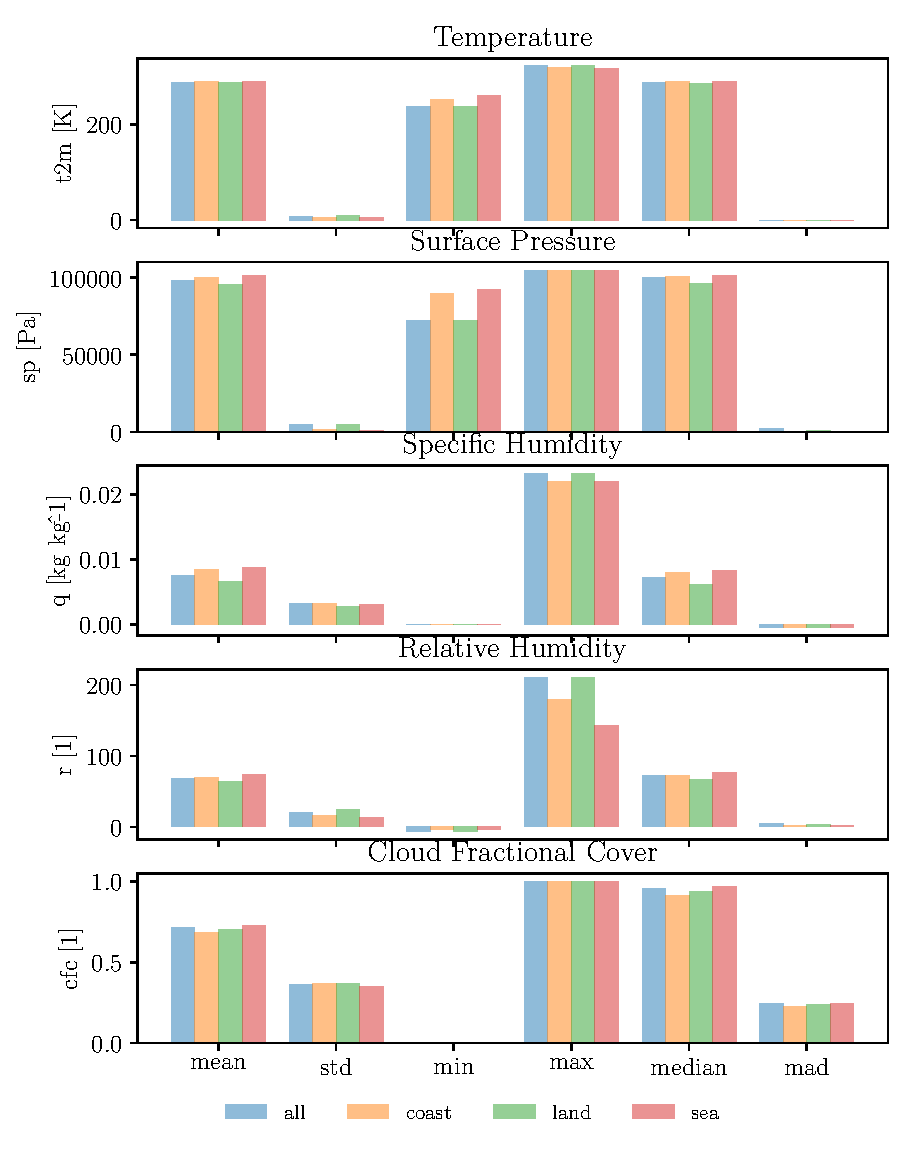
\includegraphics{python_figs/bar_plot_global_statistics_new_legend.pdf}
    \caption{Bar plot showing global statistics for different filters.}
    \label{fig:bar_plot_global_stats}
\end{figure}

\subsection{Spatial statistics}
%%%%%%%%%%%%%%%%%%%%%%%%%%%%%%%%%%% MONTHLY MEANS
Figure \ref{fig:monthly_mean_ts_vars} shows the spatially averaged monthly mean values for all values. Seasonal effects and differences between land and ocean is evident among all variables. For temperature and relative humidity, a more pronounced seasonal cycle over land, compared to ocean, is evident. The remaining variables appear to have a small shift towards higher values.
\begin{figure}[ht]
    \centering
    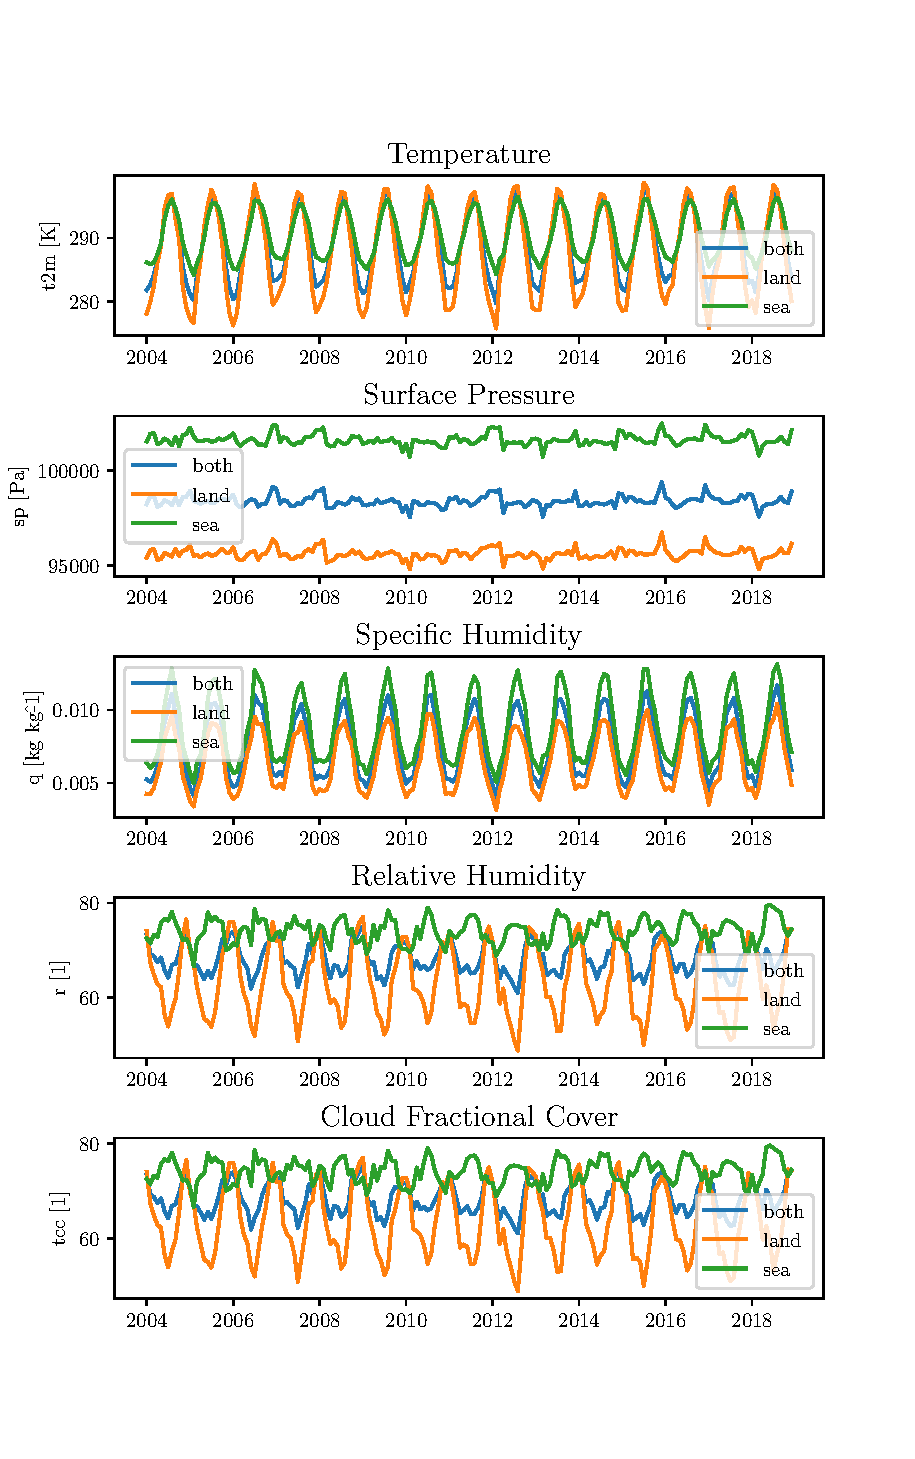
\includegraphics{python_figs/monthly_means.pdf}
    \caption{Spatially averaged monthly values. Filters are applied for land and sea.\textbf{I'm looking into why no filter is below both land and ocean and not in the middle}}
    \label{fig:monthly_mean_ts_vars}
\end{figure}

Figure \ref{fig:first_week_august_2012} shows the spatially averaged time series for the first week of August in 2012. Attempting to illustrate the relative strength of the signal feed to the input sequence. As a reference, the signal over land and ocean is provided. All variables display diurnal variations.
Because of the different intervals of the axes, the magnitude of the signal is difficult to detect from such a plot.

From the lines in 

%Surface pressure provide nearly constant values and doesn't appear to be a good predictor. If a model predicting the same value as the day before, it doesn't provide more information. \textcolor{red}{En model kan vel gi samme informasjon som dagen før så lenge observasjonene ikke endrer seg. Ser ikke ut som cloud fractional cover helle rikke endrer seg så mye eller temperaturen. Temperaturen endrer seg bare med ca. 5 grader og det er vel ikke spesielt mye? Men du vet best, ville bare reagert på at det kan være aksene som gjør at det ser ut som en stor forskjell uten at det nødvendigvis er det. }
\begin{figure}[ht]
    \centering
    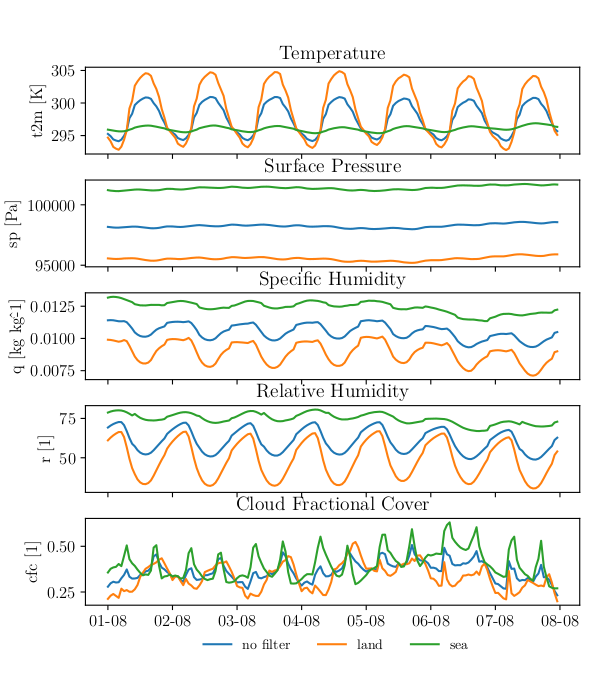
\includegraphics{python_figs/spatially_averaged_one_week_from_2012-08-01.png}
    \caption{Spatially averaged time series from the first week of August 2012.}
    \label{fig:first_week_august_2012}
\end{figure}


\subsection{Temporal statistics}
Figure \ref{fig:all_stats_tcc} shows the temporal statistics for the \acrshort{cfc} in \acrshort{ecc}. Similar figures for the remaining variables in the dataset is presented in Section \ref{sec:all_stats} in the Appendix.  The topography is a clear factor, comparing Figure \ref{fig:all_stats_tcc} to Figure \ref{fig:map} the spatial patterns are very similar. 
\textcolor{red}{Jeg så ingen veldig likhetstrekk mellom minomum value og maximum value i figur \ref{fig:all_stats_tcc}  og  Figure \ref{fig:map}. Er det feil figur eller ser jeg det bare ikke? }
\textcolor{red}{Dette er det tredje avsnittet hvor setningen starter med "Figur .... shows....". Kanskje varierer litt mer? Tenker det også er bedre om første setning er knyttet til det du vil vise. F.eks. "attempting to illustrate the relative strength of the signal feed to the input sequence, the spatially averaged time series for the first wwek in August 2012 is plotted in figure ...". DEnne ble kanskje litt lang, men noe mer sånn kan gi en bedre åpning og muligens også overgang. }
%% CLOUD FRACTIONAL COVER
\begin{figure}[ht]
    \centering
    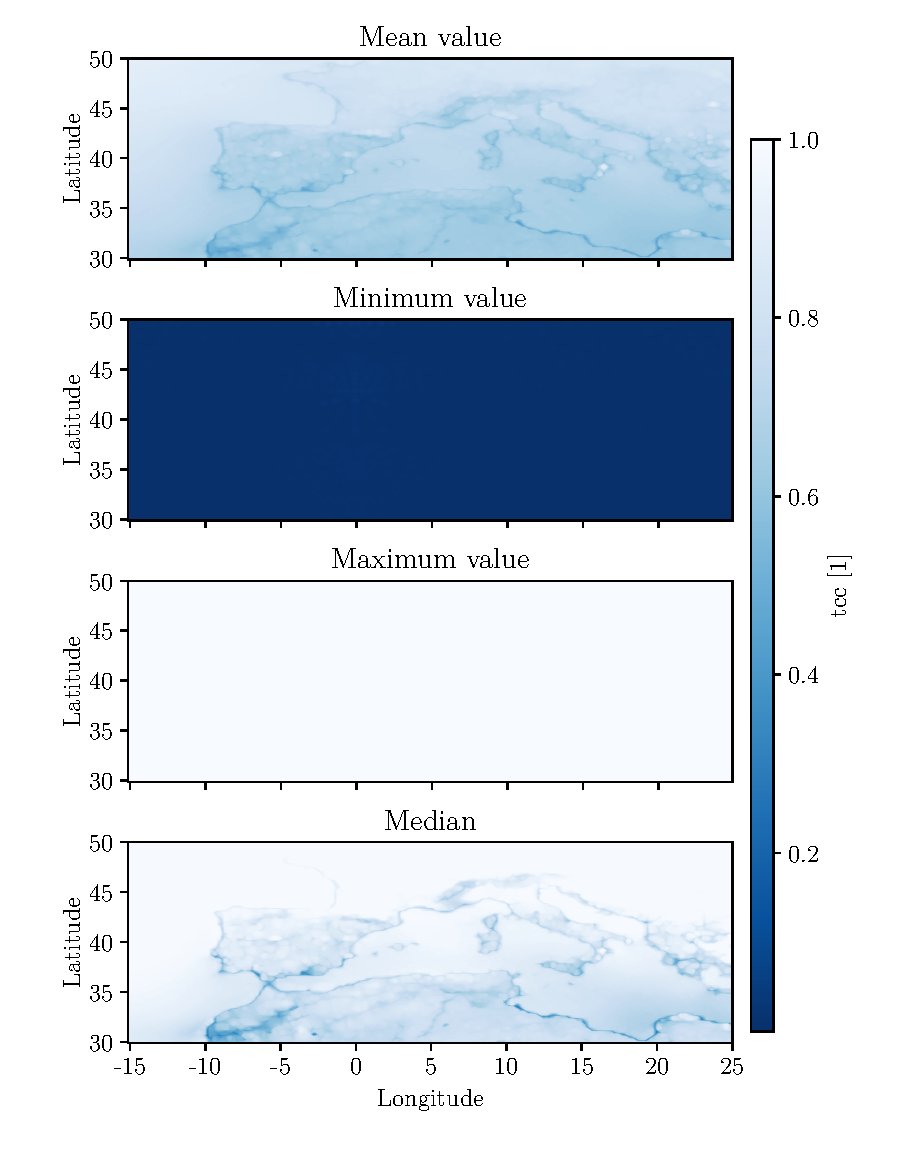
\includegraphics{python_figs/all_stat_variable_tcc.pdf}
    \caption{Contour plot showing the local (pixel) statistics for cloud fractional cover.}
    \label{fig:all_stats_tcc}
\end{figure}

The mean values, in figure \ref{fig:all_stats_tcc}, show that on average the coastline have a lower cloud cover than the adjacent areas. This is supported by the bar plot (see Figure \ref{fig:bar_plot_global_stats}). From the minimum values of cloud cover it becomes evident that there is an artefact present in the dataset. This is most likely caused by the remapping routine. Figure \ref{fig:area_pixel_signal} shows the patterns of magnitude of the areas contributing to a pixel. One might expect the contributing area to be zero over the entire domain.  One might expect the contributing area to be zero over the entire domain. However, it is not zero, meaning that these pixel have clouds at every hour in the last 14 years. The max value is as expected, one over the entire region, indicating that at some point every pixel is cloudy.

The max value is as expected, one over the entire region. It indicates that at some point every pixel is cloudy. The standard deviation is higher over land, caused by larger variation in cloud cover in these regions.

The standard deviation is higher over land, this is caused by larger variation in cloud cover in these regions. The median and \acrshort{mad} 
% Det er jo ikke rart for mad er medianen av en differanse.
show similar patterns, where the lowest values are found along the coast.

\subsubsection{Correlation between cloud cover and environmental variables}
%%% CORRELATION
Correlation describes how strong a pair of variables are linearly related. A positive correlation tells you that an increase in one variable results in an increase in the other. A negative correlation describes the opposite connection, implying that an increase in one variable cause a decrease in the other.
\begin{figure}[ht]
    \centering
    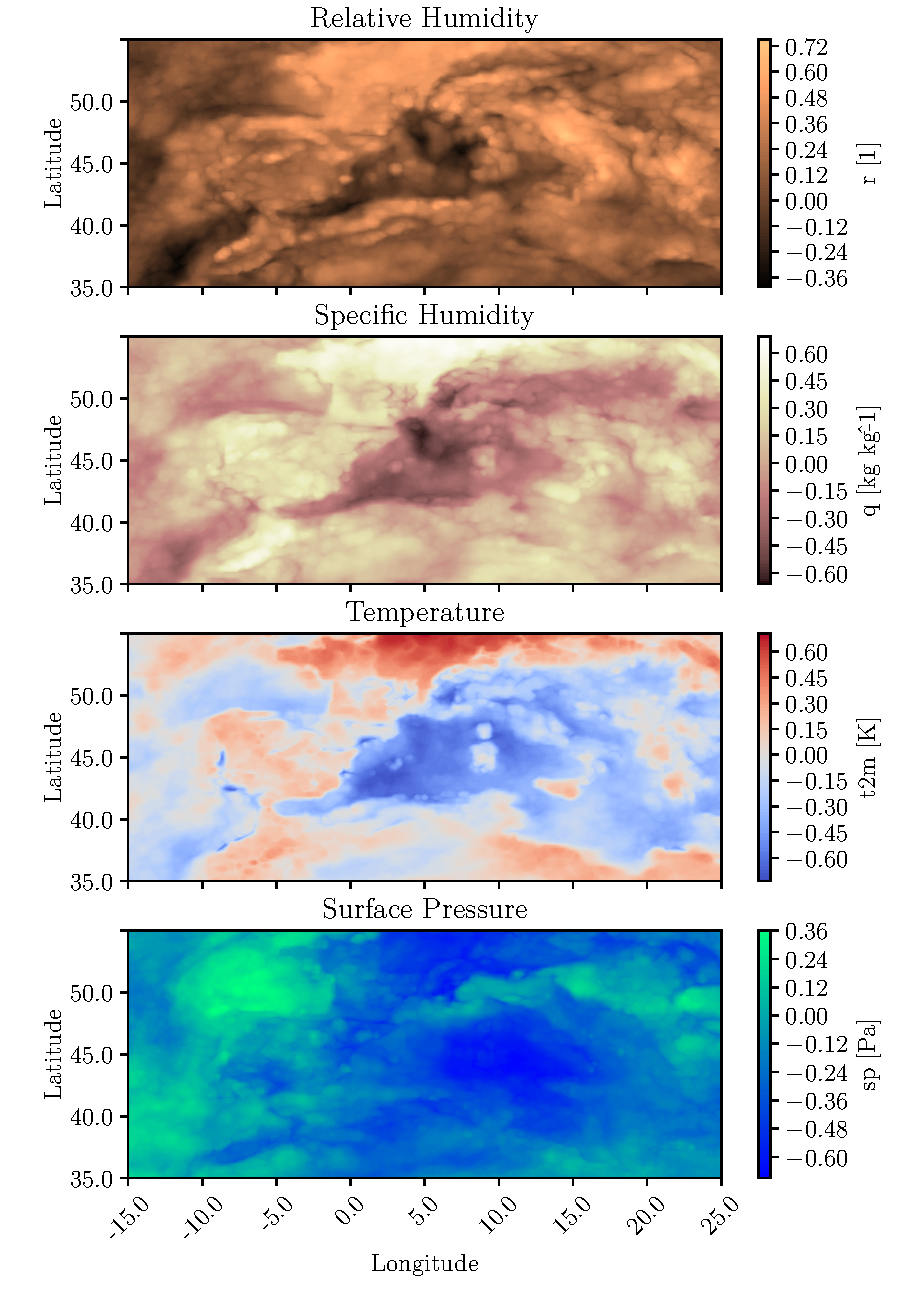
\includegraphics{python_figs/correlation_figure.pdf}
    \caption{Contour plot showing the correlation between environmental variables and cloud fractional cover.}
    \label{fig:correlation_tcc_vs_envio}
\end{figure}
Figure \ref{fig:correlation_tcc_vs_envio} shows the linear correlation coefficient from pairs of cloud cover and environmental variables such as temperature, pressure, relative and specific humidity. Recall that all environmental variables is produced by reanalysis. Pink illustrates negative correlation while green illustrates a positive correlation. Different patterns emerge from all variables. %, implying that they could be useful as predictors. 

Over land relative humidity is dominated by positive correlation to cloud cover, some part of Africa and the ocean in eastern Mediterranean has a negative correlation. The image of the surface pressure is remarkable similar, they share a pattern, but have opposite signs. The negative sign seems reasonable, since high pressure is often caused by sinking motions in the atmosphere and clouds are formed by rising motions. 

Specific humidity shows a clear shift at longitudinal degree 10. The land area in the west are negatively correlated while the eastern part are positively correlated \textcolor{red}{MEner du ikke motsatt? At i vest (west) er landområdene grønne ergo positiv korrelasjon?}. 

In most locations temperature is negatively correlated with cloud cover except in parts of the Alps, north coast of France and in north Africa. This seems reasonable since warmer air can retain more vapours, on the other hand this could enhance evaporation rate, making more vapour available for condensing onto particles. 


% Finished regriddidng files.
\section{Summary}
\acrshort{ecc} comprises of five variables; temperature, pressure, cloud fractional cover, relative and specific humidity, collected from two sources; ERA5 and EUMETSAT. The resolution available in ERA5 was preserved, while remapping the cloud mask to cloud fractions. 
% duplication
The final product consist of the variables temperature, pressure, cloud fraction, specific humidity and relative humidity, available hourly data on a $0.25^o$ uniform grid resolution in the period from April 2004 to December 2018. Cloud fractional cover (\acrshort{cfc}) is produced from area weighting cloud masks. These computations are described in Section \ref{sec:remapping}. The remaining variables are on their original format as provided by \acrfull{ecmwf}. A summary of the original sources of the dataset is given in Table \ref{tab:dataset_summary}. More details on ERA5 is available in Section \ref{sec:era5} and on Section \ref{sec:EUMETSAT_cloud_mask} for more information about cloud mask. 

\begin{table}[]
    \centering
    \resizebox{\textwidth}{!}{%
\begin{tabular}{c|c|c|c|c|}
\cline{2-5}
\multirow{4}{*}{}                                 & \multicolumn{2}{c|}{\textbf{ERA5}}                                                                                                   & \multicolumn{2}{c|}{\textbf{MSG2}}                                                                                                                \\ \cline{2-5} 
                                                  & \textbf{Type}                     & \textbf{Variables}                                                                               & \textbf{Type}                                                               & \textbf{Variables}                                                  \\ \cline{2-5} 
                                                  & Surface                           & \begin{tabular}[c]{@{}c@{}}2m Temperature\\ Surface pressure\end{tabular}                        & \multirow{2}{*}{Satelite retrival}                                          & \multirow{2}{*}{Cloud Mask}                                         \\ \cline{2-3}
                                                  & 1000 hPa                          & \begin{tabular}[c]{@{}c@{}}Relative Humidity\\ Specific Humidity\end{tabular}                    &                                                                             &                                                                     \\ \hline
\multicolumn{1}{|c|}{\textbf{Projection}}         & \multicolumn{2}{c|}{Uniform grid}                                                                                                    & \multicolumn{2}{c|}{Curve linear grid}                                                                                                            \\ \hline
\multicolumn{1}{|l|}{\textbf{Spatial resolution}} & \multicolumn{2}{c|}{$0.25^o$}                                                                                                        & \multicolumn{2}{c|}{-}                                                                                                                            \\ \hline
\multicolumn{1}{|c|}{\textbf{Output Frequencey}}  & \multicolumn{2}{c|}{Hourly}                                                                                                          & \multicolumn{2}{c|}{15 min}                                                                                                                       \\ \hline
\multicolumn{1}{|c|}{\textbf{Availability}}       & \multicolumn{2}{c|}{\begin{tabular}[c]{@{}c@{}}1979-onwards\\ Expected to be available from \\ 1950 some time in 2020.\end{tabular}} & \multicolumn{2}{c|}{2004-onward}                                                                                                                 \\ \hline
\multicolumn{1}{|c|}{\textbf{License}}           & \multicolumn{2}{c|}{\begin{tabular}[c]{@{}c@{}}Open Access. Need user \\ from Copernicus Data Storage.\end{tabular}}                  & \multicolumn{2}{c|}{\begin{tabular}[c]{@{}c@{}}Researcher Licences\\ to get 15min resolution.\\ Open access at \\ hourly resolution\end{tabular}} \\ \hline
\end{tabular}
}
\caption{Data description on the data present in the dataset ECC (European Cloud Cover). \textbf{Add projection as a column, Availability for download and the period of data.} There is a lot of work in combining the two datasets and processing it.}
\label{tab:dataset_summary}

\end{table}
%Fractional cloud cover is computed from the cloud mask product retrieved by the second generations METeosat satellites. You can read more about this data in section \ref{sec:meteosat}. For simplicity we will refer to this dataset as European Cloud Cover Dataset, ECC from now on. The visual comparison between raw satellite images and cloud amount seem to agree. The cloud fractional distribution also retain the same shape as ERA5 and MODIS 6.1 Terra in the period from 2004 to 2018. \textbf{kilde?}

%\textbf{Something is missing here -- a table?}

%\subsection{Licences and Downloading Data} \label{sec:downloading_data}
%Scripts for downloading the ERA5 data used in this thesis is available in the project GitHub on \href{https://github.com/hannasv/MS/tree/metos/downloading{\_}RA}{https://github.com/hannasv/MS/tree/metos/downloading{\_}RA}. However you will need to create a CDS-user. Follow the instructions on ECMWF homepages on \textit{how to download ERA5}. There are no scripts available for downloading METEOSAT data this is done using satellite retrievals at EUMETSATs Earth Observation Portal. Its freely available in hourly resolution. Scientist can apply for increased resolution up to 15min. Choose the cloud mask product in grb-format. By running \textbf{X - legg inn filnavn} you can generate your own files for regridding. The supplementary material only include the domain used in this thesis, because of GitHub has a maximum limit allowed for uploading. 

\cleardoublepage

%\chapter{Computer Experiments - Hugo} \label{ch:computer_experiments}
How to deal with big datasets that will easily eat up you memory? ``Big data'' involve processing large amounts of data that does not fit into memory. Processing ginormous amounts of data require expert knowledge about distributed systems and analysing for system bottlenecks. This section describes the computational experiments conducted in this study, and related issues encountered during the software development. 

%In comparison to ImageNet 2012 \textbf{source link to tensorflow docs} with downloading size is 144.02 GiB it is small. 
%However its impossible to work on the full dataset from the authors Lenovo E31 laptop. 
 %Storing is more important since the raw data used in the compilation of the dataset amount to several hundreds of Gb.

The results from the experiments conducted based on the setup and configuration. %presented in Section \ref{sec:hyperparam_tuning}.
Finally, each model is evaluated on unseen portion of the dataset. Although theoretically fascinating it remains to see if \acrshort{convlstm} provide a clear practical advantage over the autoregressive models.

\section{Hardware}
Conducting experiments on large datasets require external computational resources.  This study had access to a DGX-2 system consisting of 16 NVIDIA Tesla V100 GPUs, each of 32Gb local memory and 1.5Tb shared memory. The resources is availble through the \acrfull{ex3} project hosted at Simula. This project was awarded access 1 GPU and 1024G part of the memory. The data is stored on a \acrfull{rdma} accessed over Infiniband.
\textit{The best choice of collective implementation depends upon the number and kind of GPUs, and the network interconnect in the cluster.} The hardware sets the standard for what  efficient pipelines and training prosedyre. 
%\textit{NVIDIA V100 GPU -- The eX3 infrastructure includes a DGX-2 system consisting of 16 NVIDIA Tesla V100 GPUs, allowing simultaneous communication between all eight GPU pairs at 300 GBps through the 12 integrated NVSwitches. This gives a theoretical system-wide system bi-directional  bandwidth of 2.4 TBps. All GPUs have 32 GB of local memory (total of 512 GB) and share a 1.5 TB main memory. The total system has 81,920 CUDA cores, and 10,240 Tensor cores delivering 2 Petaflops of tensor performance. The peak performance in double precision is 125 Teraflops.}

The DGX-2 system is designed for a high level concurrency and scheduling workers competing for system resources. Working on such a monstrosity pose additional challenges related to porting existing code and virtual environments, developing and debugging code. Resulting in %a achieved 
acceptable level of efficiency and reliability. \textbf{må de siteres? (\cite{ex3docs} and \cite{ex3homepage}).} 
%\textit{This system designed for billion-way concurrency also represents a major challenge with many features: How to program such computers? How to port existing code, and how to reach a satisfactory level of reliability and efficiency while maintaining an acceptable energy footprint? How do you even debug software running on such a beast? }

%\textit{The exponentially increasing need for computing power in science and society at large has fueled the quest for developing exascale computers capable of performing a billion billion (10\textsuperscript{18}) floating-point operations per second. This upcoming generation of high performance computing (HPC) will rely on an intricate interplay between thousands of sophisticated processing nodes, each with a large number of cores, deep memory hierarchies and equipped with accelerators, organized in complex communication topologies. Heterogeneity is expected on all hardware levels, such as the nodes may also include processors that are tailored for certain types of algorithms, for instance graph-oriented methods for machine learning. While there is no fixed blueprint for exascale computers, the aggregated level of complexity in a strongly heterogeneous system designed for billion-way concurrency also represents a major challenge with many features: How to program such computers? How to port existing code, and how to reach a satisfactory level of reliability and efficiency while maintaining an acceptable energy footprint? How do you even debug software running on such a beast? While competing technologies in hardware, middleware, and software are being driven by major research projects in the United States, China, Japan and the EU, it is essential for Norwegian HPC research groups to keep pace with the frontier research.}

%\textit{The eX3 infrastructure will not be an exascale computer by itself, but it will be a carefully curated ecosystem of technology components that will be crucial for embracing exascale computing. It will allow HPC researchers throughout Norway and their collaborators to experiment hands-on with emerging HPC technologies – hardware as well as software.}

\begin{table}[ht]
    \centering
    \begin{tabular}{c|c}
        Device &  Type  \\ \hline
        GPU & Tesla V100-SXM3-32GB \\
        CPU s& DualProcessor AMD Epyc7601 (SMT2) w/2TB ram and 4TB NVMe 
    \end{tabular}
    \caption{Hardware specifications for our testing environment on eX\textsuperscript{3}. Operating system is Ubuntu 18.04.4.}
    \label{tab:hardware_ex3}
\end{table}

\section{Software}
The tensorflow keras API simplifies many aspects of building and executing machine learning models. Its implementation and distribution system aware. This makes the code more versatile, it can easily be ported to other system without many adjustments. This is not the case for the \acrshort{ar}-model and they prove to be more time consuming. \textbf{The task is performed over the entire grid,  .... legg til bedre overgang}
Distributed programming involves splitting the data into many tasks. These tasks are then executed in parallel by workers also known as threads. Parallel programming is necessary to take advantage of all the cores on a cluster to accelerate computational science. 

Complex computations will cause memory growth, dependant on how many intermediate computations it needs to store. This is the case for \acrshort{convlstm}. To speed up the development process the software is developed on a subset of \acrshort{ecc}. Small adjustments needs to be made, running experiments on the entire data. For instance threads deadlock when extracting large amounts of data. This is a precautionary measure to avoid overloading the system.

%File structure is also important, ideally data should be stored in a fashion that you don't load to much into memory. For the \acrshort{convlstm} case that would be a grid of time series, as done in this project, but for the pixelwise regression case it could be beneficially too store one pixel at a time. Storing the data in this manner will again force you to request data from the storage space more frequent, but it could ease the paralization of the program. However, there is no guarantees this will give you more bang for the buck. 


\section{Framework - Model Setup}
The following sections contain the configurations of the models compiled for this study along with descriptions of hyperparameters. A hyperparameter is a parameter set before the training starts, as mentioned in Section X. A model is compiled based on a choice of hyperparameters. In the search for the best model configuration, different combinations of hyperparameters are tested. This is done manually to begin with since the choice of architecture can easily overload the system memory resources.
%\textbf{The architecture is dependant on the problem, but also the memory resources.}

%It is possible since \acrshort{ar}-models have a small search space. The \acrshort{convlstm} models have a large search space. 
As a starting point a set of architectures used by \citeauthor{SunAirLSTM} (\citeyear{SunAirLSTM}) described in Section \ref{sec:related_work}.
%on a similar problem, air quality forecasting problem was executed. \citepaper{chollet2015kerastuner} provide suitable software for the automatic hyperparameter tuning. 
%\textbf{Man kjører eksperimenter på mange modeller ved å bruke traning og validations dataset. The choice of model is based on this data basis and then it performance is tested on the test dataset.} 

The partitioning into training and test data is inherited from the model. Since the AR-modelling is done based on a analytical solution there is no need for a validation dataset. Both model are tested on 2014 to 2018. For \acrshort{ar}-models this is trained on 2004 to 2013 and the \acrshort{convlstm} trained on  2004 to 2011 and validated on  2012 to 2013. The test period was chosen based on the assumption that the latest period is most representabel for the climate in the near future.

%Inherited from the problem the \acrshort{ar}-models dataset is split into two portions, training and test. This is sufficient, since there exist an analytical solution to this problem, as mentioned in Section \ref{sec:ARmodels}. 
%For the \acrshort{convlstm} there is no analytical solution, there is a numerical solution, this introduce the need for a validation dataset. 
Another minor differences for the datasets prepared for the \acrshort{ar} and the \acrshort{convlstm}-models. The order of the \acrshort{ar}-model determine the length of the training sequence. All samples with gaps in the requested sequence is disregarded causing a reduction in the data basis for a particular model. For the \acrshort{convlstm} these gaps are filled with a out-of-sample value, $c=1.5$.

\subsection{Autoregressive models}
%\textbf{Move first two paragraphs to discussion..?}
The python package ``sciclouds'' provide a self implemented version of \acrshort{ar}-models, using the analytical solution to the least squares problem derived in Section \ref{sec:ARmodels}. %This has major improvement possibilities. 

A set of models are compiled by varying components like scaling the predictors, transforming the target, the inclusion of intercept, order of the models and environmental variables. A summary of the calibrated models are provided in Table \ref{tab:ar_model_config}. Keep in mind that one AR-model is the combination of 13041 individual regression models.  

%Time consuming task because of the high number of matrix inversions. A double for loop over this takes to long and \textbf{mention the version of paralelization used on this problem}.
\textbf{Move this to AR model in theoretical background???}
\subsubsection{Feature Scaling} \label{sec:scaling_predictors}
%Feature standardization makes the values of each feature in the data have zero-mean 

Feature scaling is used to standardise the predictor variables.
%By subtraecting the mean and dividing by the variance, t
Applying Equation \ref{eq:scaling_data} to the predictors reshapes the distribution toward a standard normal distribution with zero mean and unit variance. 
%Data transformation can be beneficially in an attempt 
Tranformation offers an additional benefit of increased numerical stability. %When applied the predictors is transformed according to the following Equation \ref{eq:scaling_data}. 
The feature scaling is applied after the partition into training and test dataset, the mean and standard deviation is computed based on the training set. In this manner the trained model avoids sneak peaking at the test data, resulting in a unrepresentative measure on performance.
\begin{equation} \label{eq:scaling_data}
    \mathbf{x} = \frac{\mathbf{x} - \bar{\mathbf{x}}}{\sigma_{\mathbf{x}}}
\end{equation}
where $\bar{\mathbf{x}}$ is the average and $\sigma$ is the standard deviation. The model is trained to find relations in transformed data. Before making predictions based on test data it need to be transformed, using the mean and standard deviation from the training sample.

\subsubsection{Transforming target} \label{sec:transforming_target}
A trick to avoid prediction unphysical values is fitting against a transformed target. In this study, the target, \acrfull{cfc} ranges from 0 to 1. By applying the inverse sigmoid transformation, see Equation \ref{eq:sigmoid} \textbf{update to inverse sigmoid} the target takes values from the entire real axis $(-\infty, \infty)$. 
The inverse transformation, ordinary sigmoid, truncates the values back to the range [0, 1]. Thereby alleviating predictions of out-of-sample values. The sigmoid function is shown in figure \ref{fig:activation_func_plus}. 
\begin{figure}
    \centering
    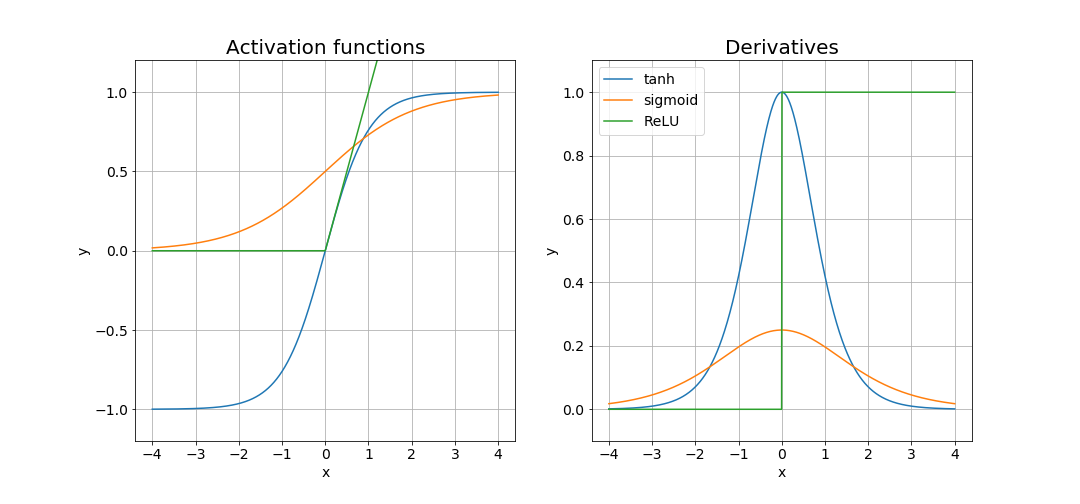
\includegraphics[scale=0.45]{Chapter3_Method/figs/activation_functions_and_derivatives.png}
    \caption{Sigmoid function and other activation functions.}
    \label{fig:activation_func_plus}
\end{figure}

\subsubsection{Order \textbf{(update to lag?)} and Environmental variables}
The dataset for a particular model is a combination of the order and whether envoirnmental variables such as $t2m$, $sp$, $q$ and $r$ is included. The eviornmental variables never appear in isolation.
Order the number of time steps of previous cloud cover includes as predictors.% and the inclusion of environmental variables, temperature, surface pressure, specific and relative humidity. 
All model is trained either on the full set of environmental variables or none of them.

\subsubsection{Experimental setup AR-models}
Table \ref{tab:ar_model_config} shows a summary of the \acrshort{ar}-models included in this study. 

\begin{table}[h]
    \centering
    \resizebox{\textwidth}{!}{%
    \begin{tabular}{ccccc}
    \cline{2-5}
     & \textbf{Scaling predictors} & \textbf{Transforming target} & \textbf{Order} & \textbf{Enviornmental variables} \\ \hline
    \multicolumn{1}{c}{\textbf{Model 1}} & \checked & $\times$  & 1 & $\times$ \\ \hline
    \multicolumn{1}{c}{\textbf{Model 2}} & \checked & $\times$  & 0 & \checked   \\ \hline
    \multicolumn{1}{c}{\textbf{Model 3}} & \checked & $\times$  & 1 & \checked  \\ \hline
    \multicolumn{1}{c}{\textbf{Model 4}} & \checked & $\times$  & 2 & \checked  \\ \hline
    \multicolumn{1}{c}{\textbf{Model 5}} & \checked & $\times$  & 3 & \checked  \\ \hline
    \multicolumn{1}{c}{\textbf{Model 6}} & \checked & $\times$  & 4 & \checked  \\ \hline
    \end{tabular}%
    }
    \caption{Configuration of \acrshort{ar}-models. $\times$ denoted not applied, \checked denotes applied \textbf{add bias??} Gi modellen navn basert på configurasjonen $AR_{STEx}$ where x is the order. \textbf{add column of number of parameters and score to avoid extra tables?}}
    \label{tab:ar_model_config}
\end{table}

\subsection{Convolutional LSTM}
The formulation of the Air quality forecasting problem presented by  \citeauthor{SunAirLSTM} is similar to the formulation of the cloud fractional cover prediction problem presented in this project. The machine learning experimental setup is adopted from the paper \citepaper{SunAirLSTM}. \textbf{Mentioned above .. remove from one of the places...}
% Endrer på arkitekturen - denne bruker -train - validation - test, en hvis prosentandel a

Citation BatchNormalization is performed between the layers \cite{ioffe2015batch}. A lot of architectural decisions (batch size, sequence length, number filterers and number layer) can cause the \acrshort{gpu} to run out of memory. In that case it didn't learn anything. 

\textbf{TODO: Add list of model configurations which actually learn something}
\begin{table}[]
    \centering
    \resizebox{\textwidth}{!}{%
    \begin{tabular}{clcccc}
     & \textbf{Sequence length} & \textbf{batchsize} & \textbf{epochs} & \textbf{MSE} & \textbf{Num Parameters} \\ \hline
    \textbf{Model 1} &  & fdfdf &  &  &  \\ \hline
    \textbf{Model 2} &  & $\checkmark$ &  &  &  \\ \hline
    \textbf{Model 2} &  &  &  &  &  \\ \hline
    \textbf{Model 2} &  &  &  &  &  \\ \hline
    \textbf{Model 2} &  &  &  &  &  \\ \hline
    \textbf{Model 2} &  &  &  &  &  \\ \hline
    \end{tabular}%
    }
    \caption{Configuration of traninable convolutional lstm models. \textbf{r2 er veldig merkelig foreløbig, includere mae?}}
    \label{tab:convlstm_config}
\end{table}

\section{Results}
\textbf{Føler det er unødvendig med ekstra tabeller her når du passe så lett sammen med model configurasjons tabellene. Det blir også lettere å tolke om det står sammen.. Hva tenker du..? }

This section presents comparisons from the best convolutional lstm model and the best AR-model. Recall that the Convolutional LSTM model is chosen based on its score of predicting the sequence length and the AR-model is currently evaluated on its performance predicting one step a head. \textbf{Dette er en mismatch som kanskje bør ryddes opp i ..}

\subsection{Predicting next timestep -- remove or train convlstm model to predict one step}
Currently not made any conv lstm models predicting one step ahead....
%%%% TARGET PREDICITON ERA5
\begin{figure}[ht]
    \centering
    \includegraphics{python_figs/target_prediction_era5_plot_horizonal.pdf}
    \caption{Comparison target, predicted and era5 horizontal cloud fractional cover. Imagine this plot, with a row for each step in the predicted sequence and each column being (AR, Convlstm, target)}
    \label{fig:target_predict_era5_horizontal}
\end{figure}



\subsection{Predicting next 24 hours (or another sequence depend on which models learns this)}
%%%% TARGET PREDICITON ERA5
\begin{figure}[ht]
    \centering
    \includegraphics{python_figs/target_prediction_era5_plot_horizonal.pdf}
    \caption{Comparison target, predicted and era5 horizontal cloud fractional cover. Imagine this plot, with a row for each step in the predicted sequence and each column being (AR, Convlstm, target)}
    \label{fig:target_predict_era5_horizontal}
\end{figure}



\subsection{Autoregressive models}

%%%% TARGET PREDICITON HORIZONTAL
\begin{figure}[ht]
    \centering
    \includegraphics{python_figs/target_prediction_plot_horizonal.pdf}
    \caption{Comparison target and predicted cloud fractional cover.}
    \label{fig:target_predict_horizontal}
\end{figure}

%%%% TARGET PREDICITON HORIZONTAL
\begin{figure}[ht]
    \centering
    \includegraphics{python_figs/target_prediction_plot_vertical.pdf}
    \caption{Comparison target and predicted vertical cloud fractional cover.}
    \label{fig:target_predict_vertical}
\end{figure}



\subsection{Convolutional Long Short-Term Memory network}
Either summaries the findings into one table 


\section{Experiments}





\section{Practical implications - OUTDATED} \label{sec:practical_implications}
It is necessary to have a understanding of the needs of the end product before conducting large machine learning projects. Answering questions like: What will it be used for and how can it be implemented in useful way?

A major downside of the data driven learning approach is the rigid resolution. A trained model can only be used on similar problems, with the same spatiotemporal resolution. For applications like climate models, output comes in a wide range of different resolutions. Before implementing the finished product in a new model of a different resolution, it would need to be retrained on the resolution of the climate model under development. This process involves both remapping of the dataset and retraining the model at the correct resolution. This is a time consuming process involving finding a new set of hyperparameters suitable for the new resolution. % It essentially means starting over.

Once trained on global climate datasets, machine learning models provide fast results even for complex parameterization which is what makes them suitable for the application of climate modelling. Most machine learning packages are developed using Python. \acrfull{esm} are implemented in python. Methods for including the trained parameterizations need to be developed.
 
\subsection{Any implications based on the results presented in this chapter.}
\cleardoublepage

%\chapter{Conclusions}

\section{Summary of contributions and main findings }
State something great about the dataset.



\section{Future work}

In future work it would be interesting to asses how data driven parametrisation compare to the existing parametrisaions available in the state of the art climate models. Here both the temporal and spatial resolution is a lot coarser. Other data sets could be considered. The masks in other data sets are computed based on more channels than in METeosat but the temporal resolution is a lot worse. 



\section{Final remark}
Text
\cleardoublepage

%\appendix
\chapter{Statistics} \label{ch:appendix_statistic}
TODO: Rewrite this to contain plots of one variables divided into statistics and deviation - both having a single colorbar on the right

\section{Temporal statistics} \label{sec:all_stats}
%%% ALL LOCAL STATISTICS FOR VARIABLES 
%% TEMPERATURE
\begin{figure}[ht]
    \centering
    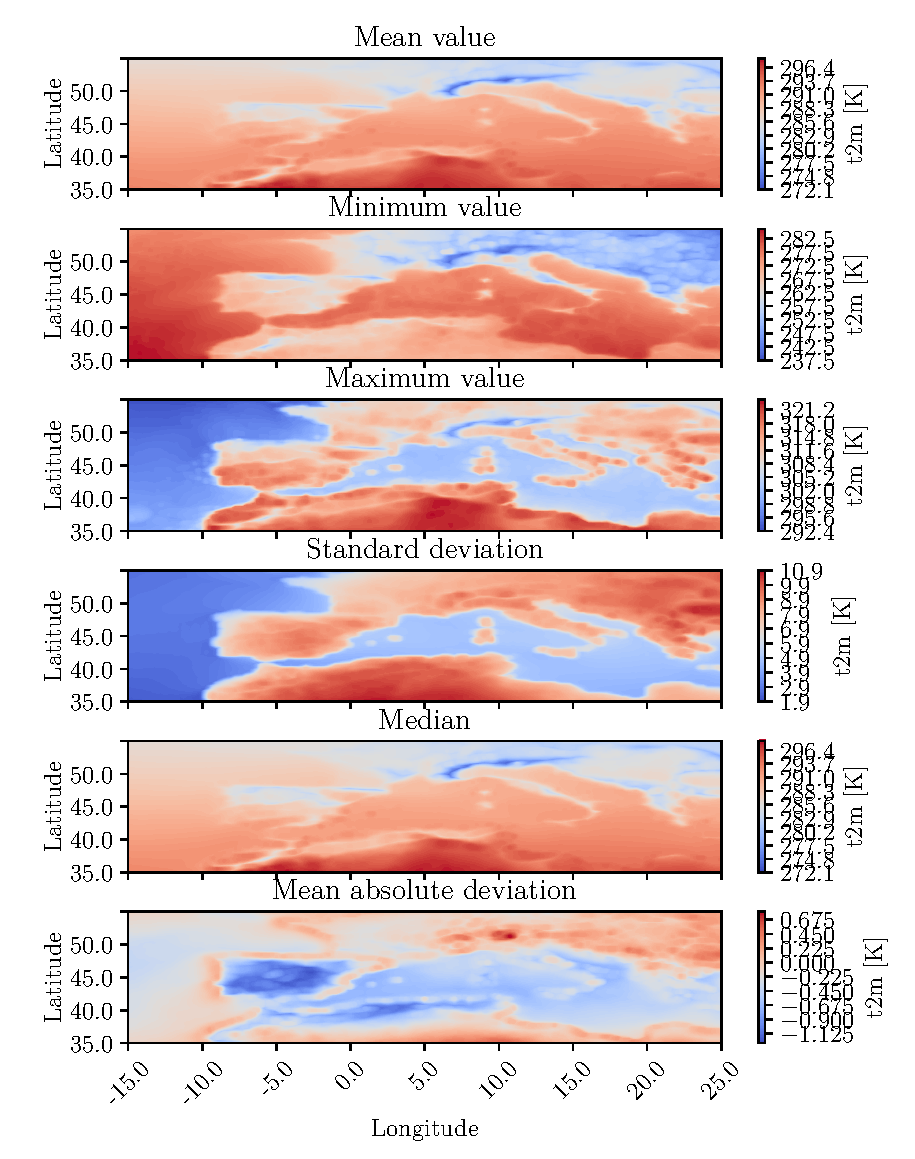
\includegraphics{python_figs/all_stat_variable_t2m.pdf}
    \caption{Contour plot showing the local (pixel) statistics for temperature.}
    \label{fig:all_stats_t2m}
\end{figure}

%% SURFACE PRESSURE 
\begin{figure}[ht]
    \centering
    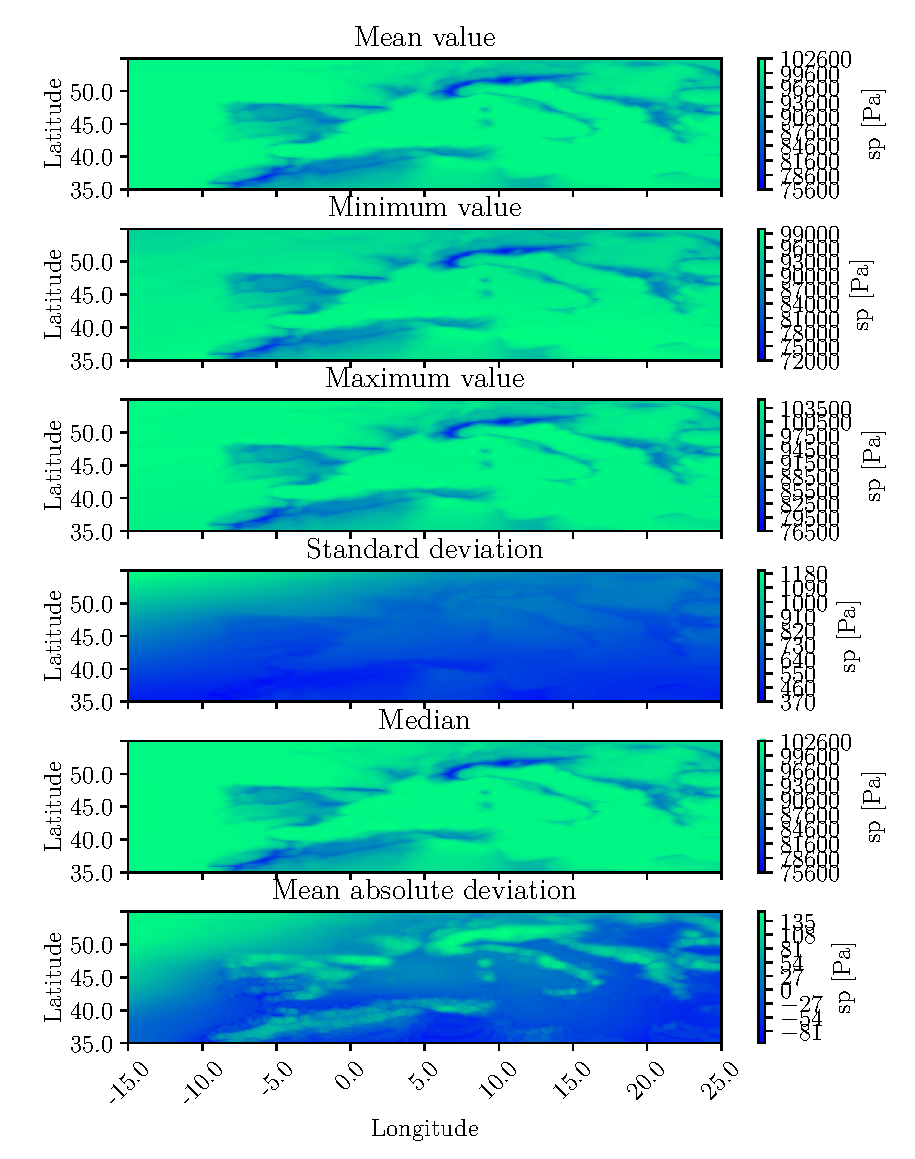
\includegraphics{python_figs/all_stat_variable_sp.pdf}
    \caption{Contour plot showing the local (pixel) statistics for surface pressure.}
    \label{fig:all_stats_sp}
\end{figure}

%% RELATIVE HUMIDITY 
\begin{figure}[ht]
    \centering
    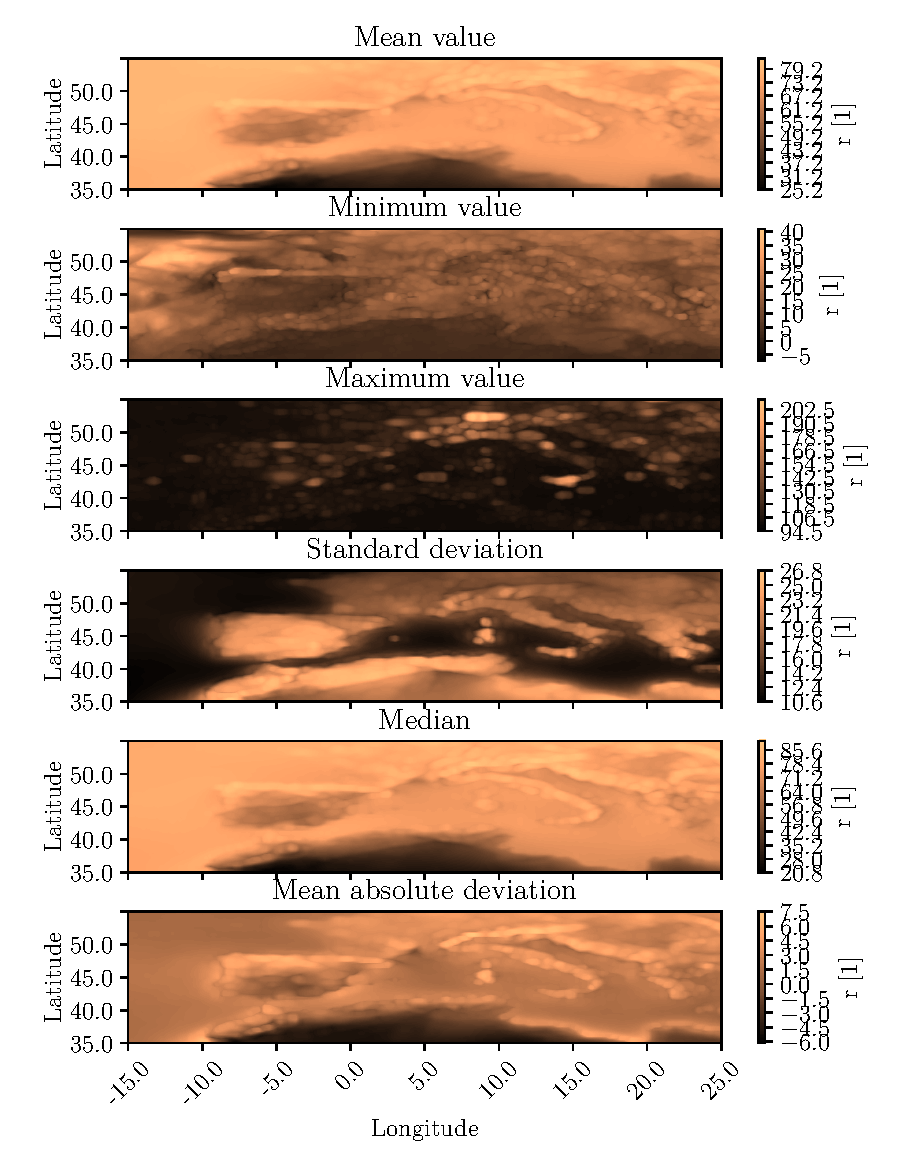
\includegraphics{python_figs/all_stat_variable_r.pdf}
    \caption{Contour plot showing the local (pixel) statistics for relative humidity.}
    \label{fig:all_stats_r}
\end{figure}

%% SPECIFIC HUMIDITY 
\begin{figure}[ht]
    \centering
    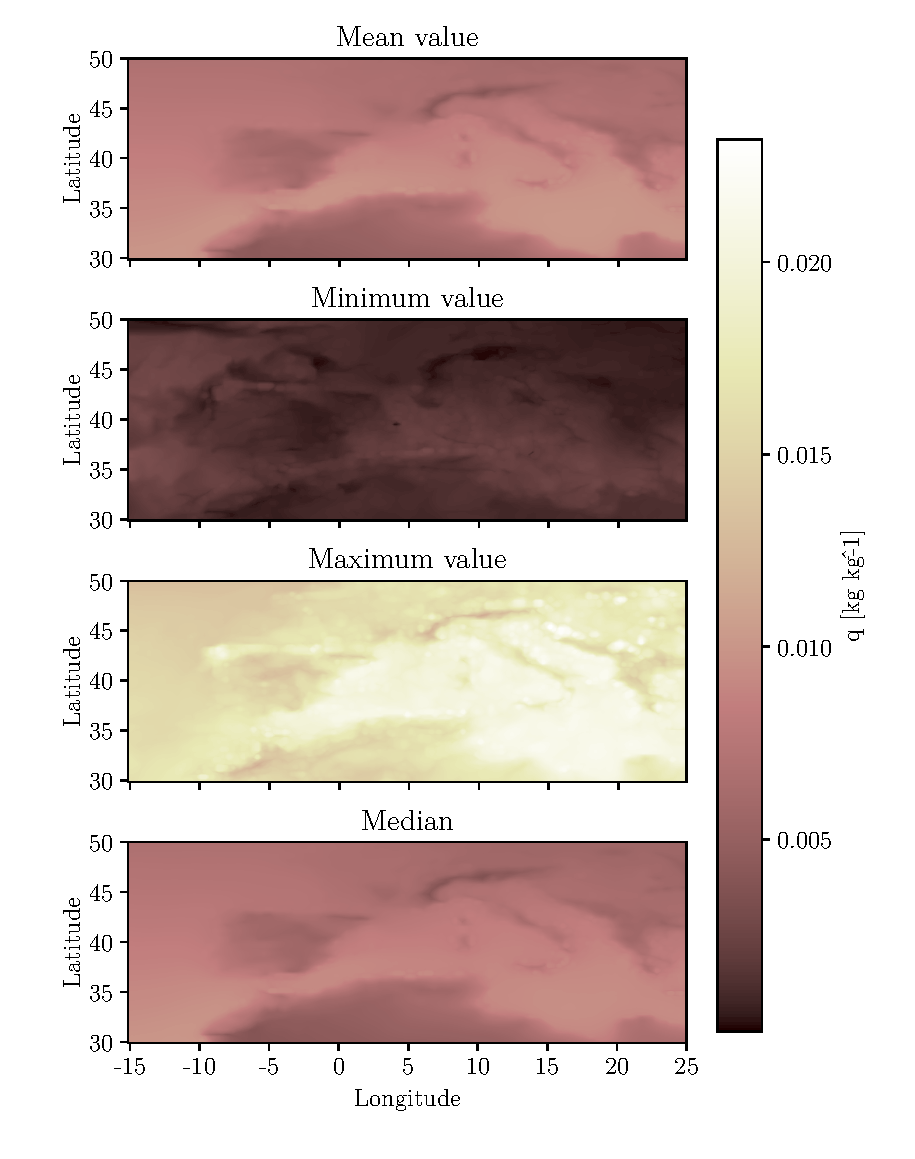
\includegraphics{python_figs/all_stat_variable_q.pdf}
    \caption{Contour plot showing the local (pixel) statistics for specific humidity.}
    \label{fig:all_stats_q}
\end{figure}

\section{Temporal statistics deviations} \label{sec:all_stats_deviation}
\begin{figure}
    \centering
    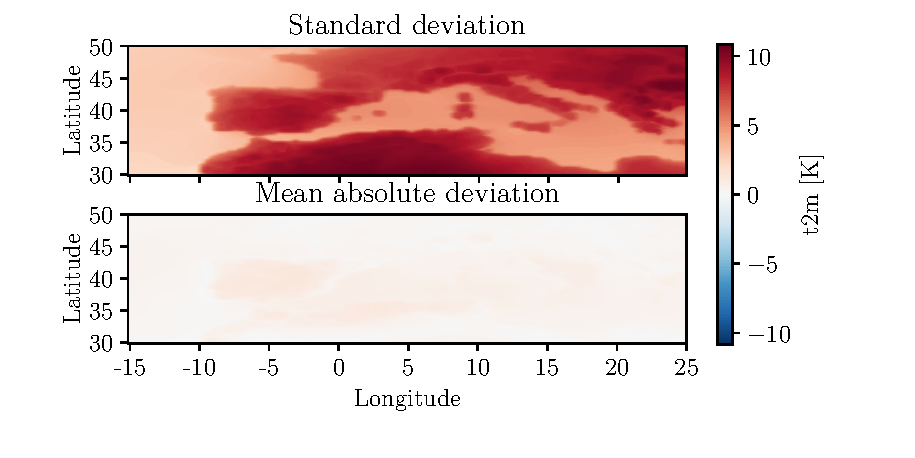
\includegraphics{python_figs/DEVIATION_all_stat_variable_t2m.pdf}
    \caption{Deviations in tempreature, t2m.}
    \label{fig:deviation_t2m}
\end{figure}

\begin{figure}
    \centering
    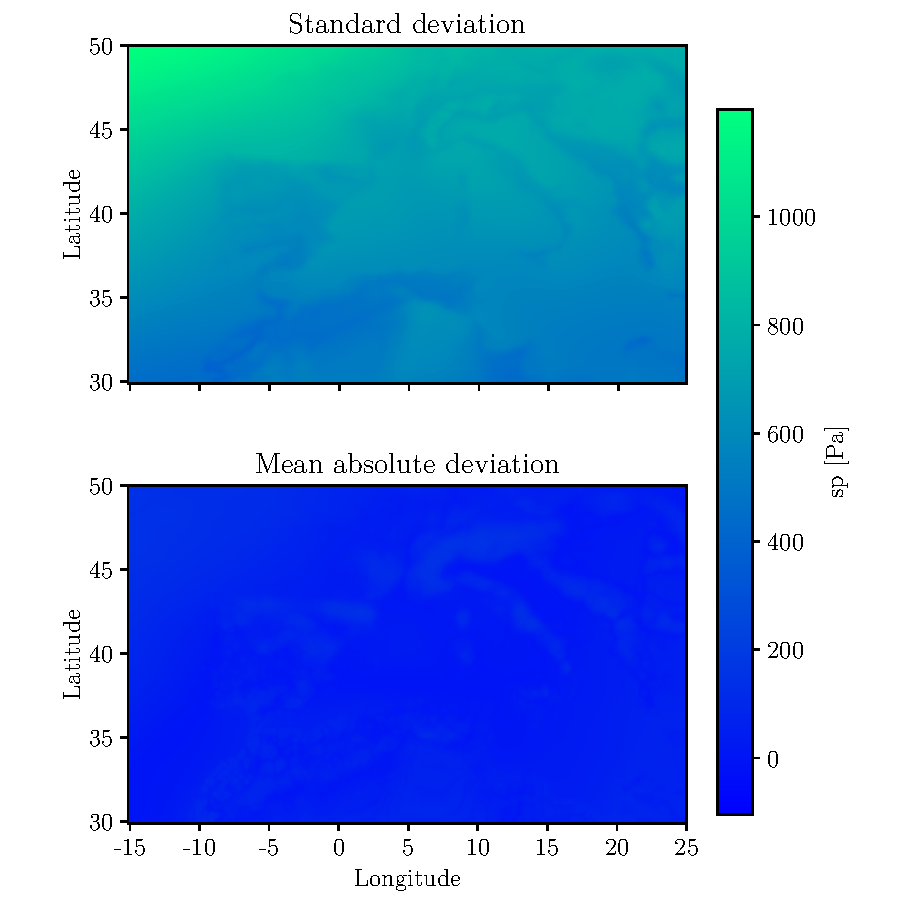
\includegraphics{python_figs/DEVIATION_all_stat_variable_sp.pdf}
    \caption{Deviations in surface pressure, sp.}
    \label{fig:deviation_sp}
\end{figure}

\begin{figure}
    \centering
    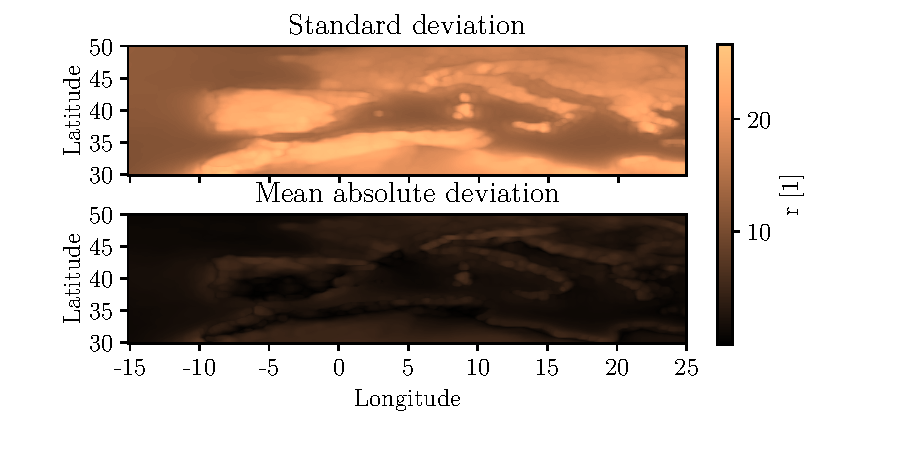
\includegraphics{python_figs/DEVIATION_all_stat_variable_r.pdf}
    \caption{Deviations in relative humidity, r.}
    \label{fig:deviation_r}
\end{figure}


\begin{figure}
    \centering
    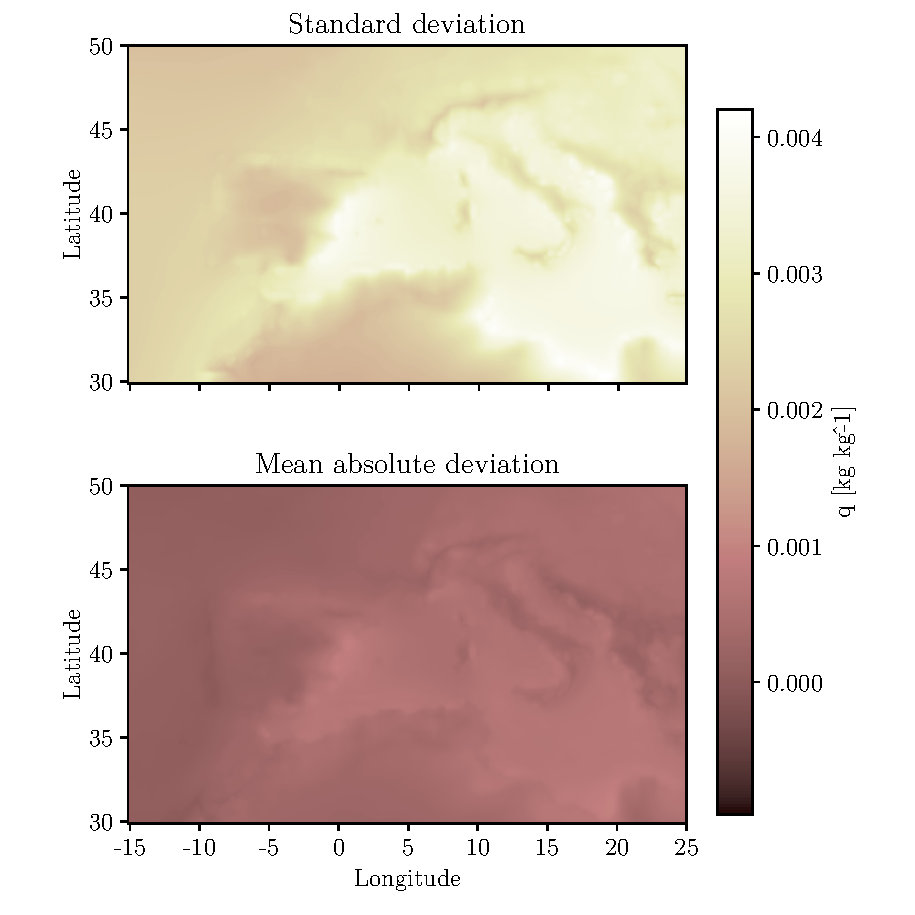
\includegraphics{python_figs/DEVIATION_all_stat_variable_q.pdf}
    \caption{Deviations in specific humidity, q.}
    \label{fig:deviation_q}
\end{figure}


\cleardoublepage

\chapter{Seasonal effects}
This section has more plots. 
\begin{figure}[ht]
    \centering
    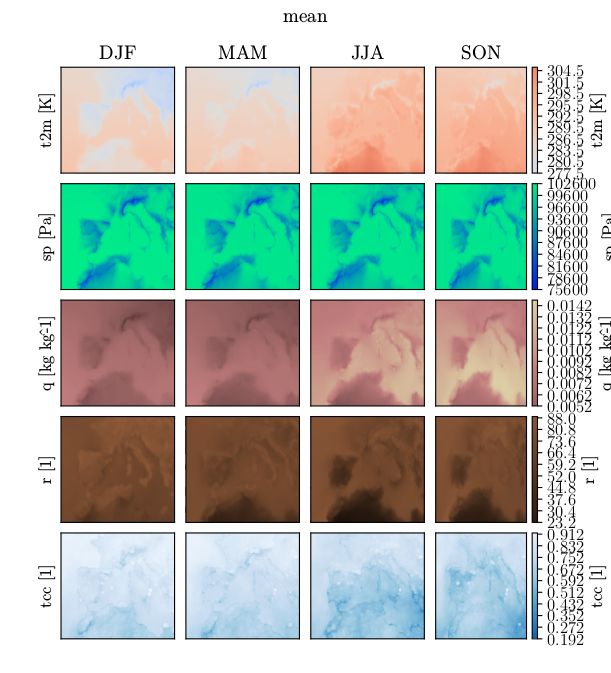
\includegraphics{python_figs/seasonal_mean_all_variables.png}
    \caption{Seasonal mean}
    \label{fig:seasonal_mean}
\end{figure}

\begin{figure}[ht]
    \centering
    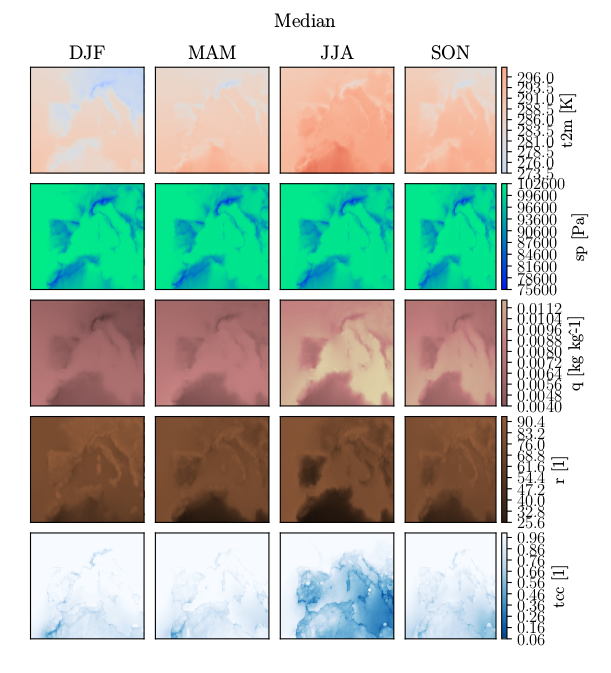
\includegraphics{python_figs/seasonal_median_all_variables.png}
    \caption{Seasonal median}
    \label{fig:seasonal_median}
\end{figure}

\chapter{Performance of other models}
Currently it show the plots that could be generated to show the performance for other model. The plots below is generated based on dummy data. 

%%%% TARGET PREDICITON HORIZONTAL
\begin{figure}[ht]
    \centering
    \includegraphics{python_figs/target_prediction_plot_horizonal.pdf}
    \caption{Comparison target and predicted cloud fractional cover.}
    \label{fig:target_predict_horizontal}
\end{figure}

%%%% TARGET PREDICITON HORIZONTAL
\begin{figure}[ht]
    \centering
    \includegraphics{python_figs/target_prediction_plot_vertical.pdf}
    \caption{Comparison target and predicted vertical cloud fractional cover.}
    \label{fig:target_predict_vertical}
\end{figure}

%%%% TARGET PREDICITON ERA5
\begin{figure}[ht]
    \centering
    \includegraphics{python_figs/target_prediction_era5_plot_horizonal.pdf}
    \caption{Comparison target, predicted and era5 horizontal cloud fractional cover.}
    \label{fig:target_predict_era5_vertical}
\end{figure}

\cleardoublepage


\chapter{Time lapse of \acrlong{cfc}. }

\begin{figure}[ht]
    \centering
    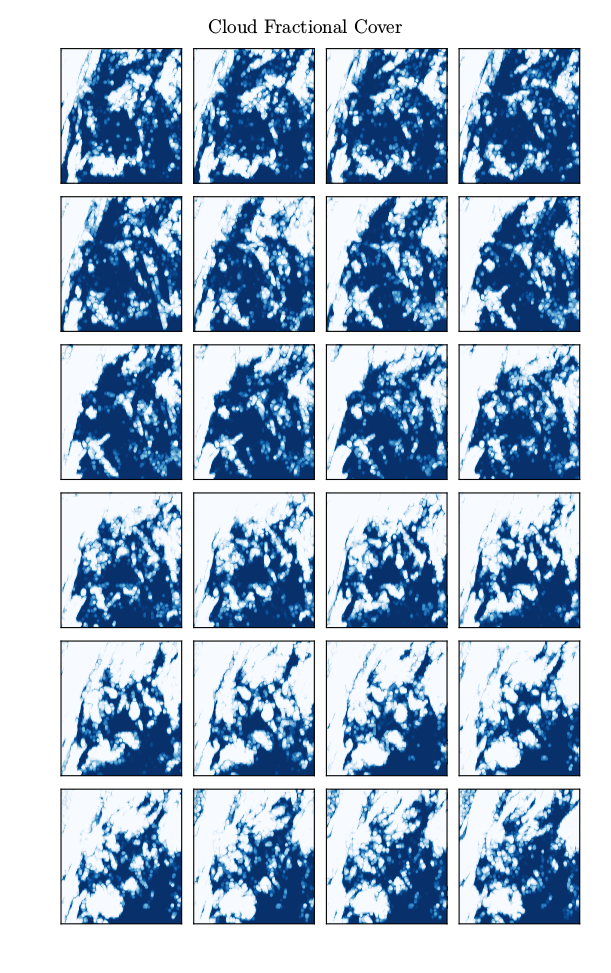
\includegraphics[scale=0.7]{python_figs/timelapse_cloud_cover_24hrs_from_2010-07-01.png}
    \caption{Time lapse photo, trying to detect the signal you would get from cloud cover within 24 hours.}
    \label{fig:time_lapse}
\end{figure}



\chapter{First week of every month in 2012} \label{app:first_week}
%\addcontentsline{toc}{chapter}{Appendix D: Study 2012}

\begin{figure}[ht]
    \centering
    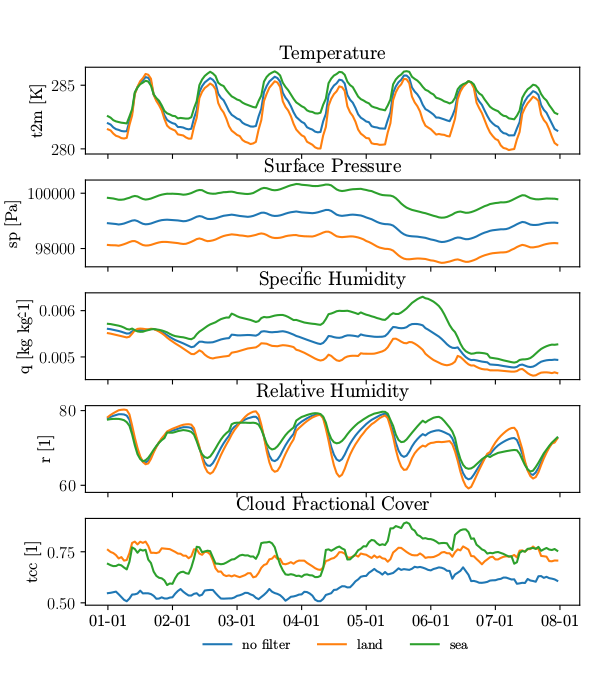
\includegraphics{python_figs/spatially_averaged_one_week_from_2012-01-01.png}
    \caption{Signal January 2012.}
    \label{fig:jan12}
\end{figure}

\begin{figure}[ht]
    \centering
    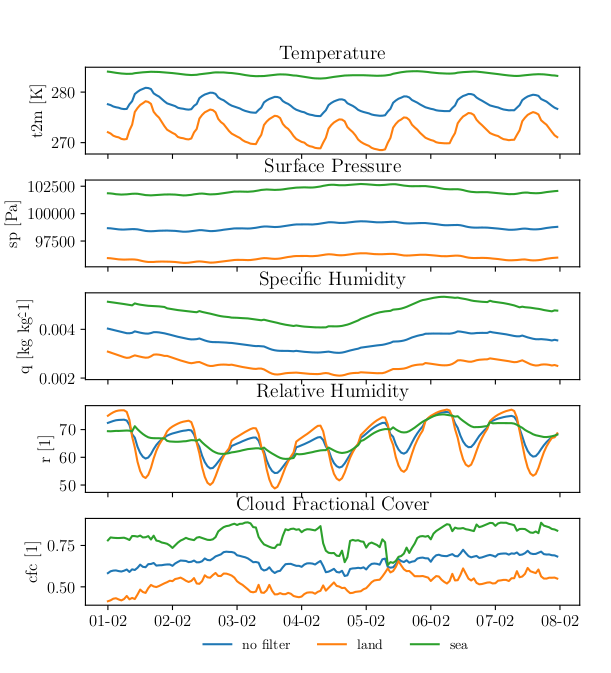
\includegraphics{python_figs/spatially_averaged_one_week_from_2012-02-01.png}
    \caption{Signal February 2012.}
    \label{fig:feb12}
\end{figure}

\begin{figure}[ht]
    \centering
    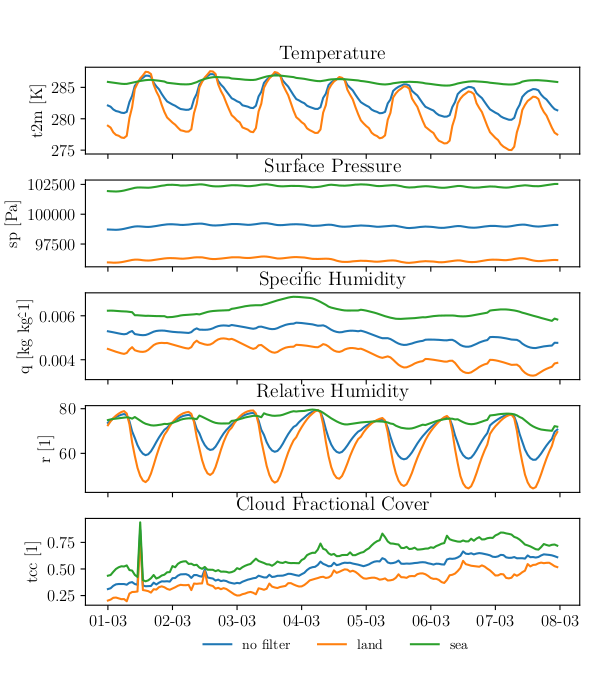
\includegraphics{python_figs/spatially_averaged_one_week_from_2012-03-01.png}
    \caption{Signal March 2012.}
    \label{fig:mar12}
\end{figure}

\begin{figure}[ht]
    \centering
    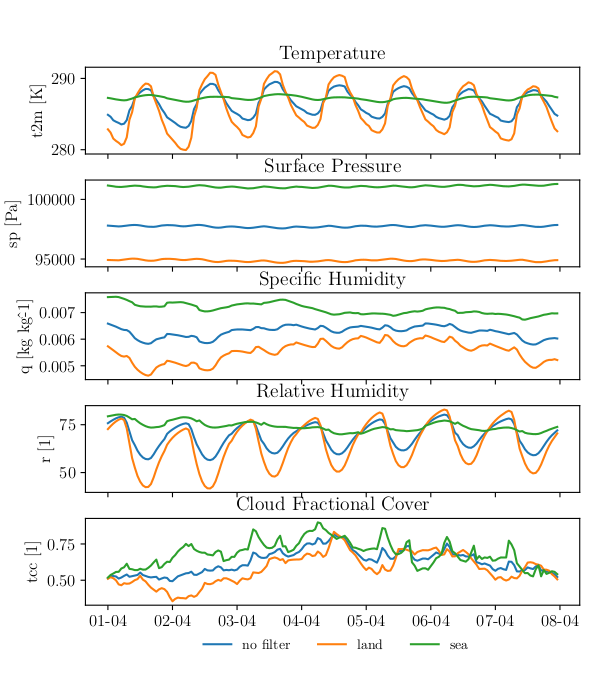
\includegraphics{python_figs/spatially_averaged_one_week_from_2012-04-01.png}
    \caption{Signal April 2012.}
    \label{fig:april12}
\end{figure}

\begin{figure}[ht]
    \centering
    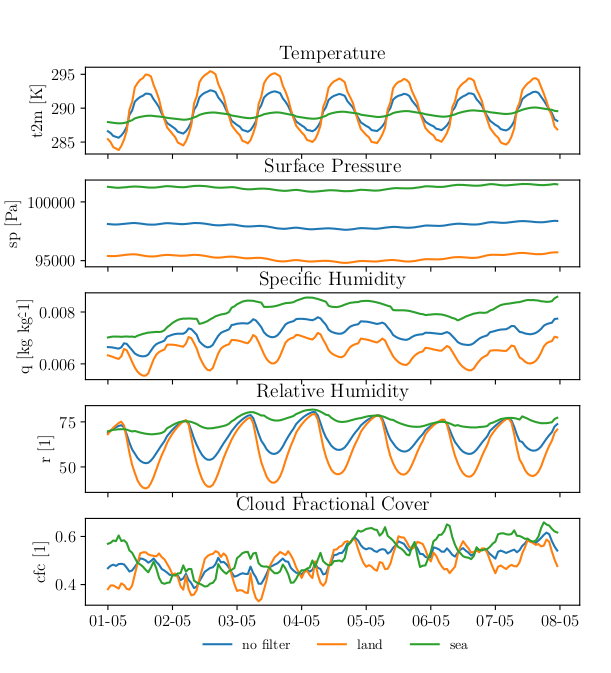
\includegraphics{python_figs/spatially_averaged_one_week_from_2012-05-01.png}
    \caption{Signal May 2012.}
    \label{fig:may12}
\end{figure}


\begin{figure}[ht]
    \centering
    \includegraphics{python_figs/spatially_averaged_one_week_from_2012-06-01.png}
    \caption{Signal June 2012.}
    \label{fig:jun12}
\end{figure}

\begin{figure}[ht]
    \centering
    \includegraphics{python_figs/spatially_averaged_one_week_from_2012-07-01.png}
    \caption{Signal July 2012.}
    \label{fig:jul12}
\end{figure}


\begin{figure}[ht]
    \centering
    \includegraphics{python_figs/spatially_averaged_one_week_from_2012-08-01.png}
    \caption{Signal August 2012.}
    \label{fig:aug12}
\end{figure}

% September is in the text

\begin{figure}[ht]
    \centering
    \includegraphics{python_figs/spatially_averaged_one_week_from_2012-10-01.png}
    \caption{Signal October 2012.}
    \label{fig:oct12}
\end{figure}


\begin{figure}[ht]
    \centering
    \includegraphics{python_figs/spatially_averaged_one_week_from_2012-11-01.png}
    \caption{Signal November 2012.}
    \label{fig:nov12}
\end{figure}

\begin{figure}[ht]
    \centering
    \includegraphics{python_figs/spatially_averaged_one_week_from_2012-12-01.png}
    \caption{Signal December 2012.}
    \label{fig:dec12}
\end{figure}

\cleardoublepage

\chapter{All four parts of example prediction} \label{app:pred_sequence}
\textbf{OBS this duplicates the first one}

\begin{figure}
    \centering
    \includegraphics{python_figs/comparting_seq_part_1_of4.png}
    \caption{Part 1/4 of the predicted 24 hours sequence }
    \label{fig:part1/4}
\end{figure}

%\begin{figure}
%    \centering
%    \includegraphics{python_figs/comparting_seq_part_2_of4.png}
%    \caption{Part 2/4 of the predicted 24 hours sequence }
%    \label{fig:part2/4}
%\end{figure}

%\begin{figure}
%    \centering
%    \includegraphics{python_figs/comparting_seq_part_3_of4.png}
%    \caption{Part 3/4 of the predicted 24 hours sequence }
%    \label{fig:part3/4}
%\end{figure}

\begin{figure}
    \centering
    \includegraphics{python_figs/comparting_seq_part_4_of4.png}
    \caption{Part 4/4 of the predicted 24 hours sequence }
    \label{fig:part4/4}
\end{figure}

\cleardoublepage

%%%%%%%%%%%%%%%%%%%%%%%%%%%%%%%%%%%%% signal artefact should be redefined if used 
\chapter{Miscellaneous} \label{app:misc}

\begin{figure}
    \centering
    \includegraphics{python_figs/signal_artefact.png}
    \caption{Occurrence of artefact, keep in mind that is not made any effort to distinguish this from when the entire area has cloud cover, this could be done by the ratio of artefact signal to land or something else. }
    \label{fig:signal_artefact}
\end{figure}

\cleardoublepage

\addcontentsline{toc}{chapter}{Bibliography}
\printbibliography
\cleardoublepage

\end{document}
